\def\paperversiondraft{draft}
\def\paperversionblind{blind}
\def\paperversioncamera{camera}

% If no special paper-version is requested, compile in draft mode
\ifx\paperversion\paperversionblind
\else
  \ifx\paperversion\paperversioncamera
  \else
     \def\paperversion{draft}
  \fi
\fi

\def\grammarlyon{on}

\ifx\grammarly\grammarlyon
\def\review{}
\else
\def\review{review,}
\fi

\ifx\paperversion\paperversiondraft
  \documentclass[sigplan,\review anonymous]{acmart}
\fi

\ifx\paperversion\paperversionblind
  \documentclass[sigplan,\review anonymous]{acmart}
\fi

\ifx\paperversion\paperversioncamera
  \documentclass[sigplan]{acmart}\settopmatter{}
\fi

\usepackage{colortbl}
\usepackage{xargs}
\usepackage{lipsum}
\usepackage[textsize=tiny]{todonotes}
\usepackage{xparse}
\usepackage{xifthen, xstring}
\usepackage{ulem}
\usepackage{xspace}

\usepackage{listings}
\usepackage{algpseudocode}
\usepackage{algorithm}
\usepackage{graphicx} %package to manage images

\lstset{
  numbers=left,
  stepnumber=1,    
  firstnumber=1,
  numberfirstline=true,
  xleftmargin=2em,
  framexleftmargin=1.5em
}

\NewDocumentCommand{\INTERVALINNARDS}{ m m }{
    #1 {,} #2
}
\NewDocumentCommand{\interval}{ s m >{\SplitArgument{1}{,}}m m o }{
    \IfBooleanTF{#1}{
        \left#2 \INTERVALINNARDS #3 \right#4
    }{
        \IfValueTF{#5}{
            #5{#2} \INTERVALINNARDS #3 #5{#4}
        }{
            #2 \INTERVALINNARDS #3 #4
        }
    }
}

\newcommand*{\thead}[1]{\multicolumn{1}{c}{\bfseries #1}}

\makeatletter
\font\uwavefont=lasyb10 scaled 652

\newcommand\colorwave[1][blue]{\bgroup\markoverwith{\lower3\p@\hbox{\uwavefont\textcolor{#1}{\char58}}}\ULon}
\makeatother

\ifx\paperversion\paperversiondraft
\newcommand\createtodoauthor[2]{%
\def\tmpdefault{emptystring}
\expandafter\newcommand\csname #1\endcsname[2][\tmpdefault]{\def\tmp{##1}\ifthenelse{\equal{\tmp}{\tmpdefault}}
   {\todo[linecolor=#2,backgroundcolor=#2,bordercolor=#2]{\textbf{#1:} ##2}}
   {\ifthenelse{\equal{##2}{}}{\colorwave[#2]{##1}\xspace}{ \todo[linecolor=#2,backgroundcolor=#2,bordercolor=#2]{\textbf{#1:} ##2}\colorwave[#2]{##1}}}}}
\else
\newcommand\createtodoauthor[2]{%
\def\tmpdefault{emptystring}
\expandafter\newcommand\csname #1\endcsname[2][\tmpdefault]{\def\tmp{##1}\ifthenelse{\equal{\tmp}{\tmpdefault}}
   {}
   {\ifthenelse{\equal{##2}{}}{##1\xspace}{ ##1}}}}
\fi

% Broaden margins to make room for todo notes
\ifx\paperversion\paperversiondraft
  \paperwidth=\dimexpr \paperwidth + 6cm\relax
  \oddsidemargin=\dimexpr\oddsidemargin + 3cm\relax
  \evensidemargin=\dimexpr\evensidemargin + 3cm\relax
  \marginparwidth=\dimexpr \marginparwidth + 3cm\relax
  \setlength{\marginparwidth}{4.6cm}
\fi

% We use the following color scheme
% 
% This scheme is both print-friendly and colorblind safe for
% up to four colors (including the red tones makes it not
% colorblind safe any more)
%
% https://colorbrewer2.org/#type=qualitative&scheme=Paired&n=4

\definecolor{pairedOneLightBlue}{HTML}{a6cee3}
\definecolor{pairedTwoDarkBlue}{HTML}{1f78b4}
\definecolor{pairedThreeLightGreen}{HTML}{b2df8a}
\definecolor{pairedFourDarkGreen}{HTML}{33a02c}
\definecolor{pairedFiveLightRed}{HTML}{fb9a99}
\definecolor{pairedSixDarkRed}{HTML}{e31a1c}

\createtodoauthor{grosser}{pairedOneLightBlue}
\createtodoauthor{authorTwo}{pairedTwoDarkBlue}
\createtodoauthor{authorThree}{pairedThreeLightGreen}
\createtodoauthor{authorFour}{pairedFourDarkGreen}
\createtodoauthor{authorFive}{pairedFiveLightRed}
\createtodoauthor{authorSix}{pairedSixDarkRed}

%% Note: Authors migrating a paper from traditional SIGPLAN
%% proceedings format to PACMPL format should change 'sigplan' to
%% 'acmsmall'.


%% Some recommended packages.
\usepackage{booktabs}   %% For formal tables:
                        %% http://ctan.org/pkg/booktabs
\usepackage{subcaption} %% For complex figures with subfigures/subcaptions
                        %% http://ctan.org/pkg/subcaption


\makeatletter\if@ACM@journal\makeatother
%% Journal information (used by PACMPL format)
%% Supplied to authors by publisher for camera-ready submission
\acmJournal{PACMPL}
\acmVolume{1}
\acmNumber{1}
\acmArticle{1}
\acmYear{2017}
\acmMonth{1}
\acmDOI{10.1145/nnnnnnn.nnnnnnn}
\startPage{1}
\else\makeatother
%% Conference information (used by SIGPLAN proceedings format)
%% Supplied to authors by publisher for camera-ready submission
\acmConference[PL'17]{ACM SIGPLAN Conference on Programming Languages}{January 01--03, 2017}{New York, NY, USA}
\acmYear{2017}
\acmISBN{978-x-xxxx-xxxx-x/YY/MM}
\acmDOI{10.1145/nnnnnnn.nnnnnnn}
\startPage{1}
\fi


%% Copyright information
%% Supplied to authors (based on authors' rights management selection;
%% see authors.acm.org) by publisher for camera-ready submission
\setcopyright{none}             %% For review submission
%\setcopyright{acmcopyright}
%\setcopyright{acmlicensed}
%\setcopyright{rightsretained}
%\copyrightyear{2017}           %% If different from \acmYear


%% Bibliography style
\bibliographystyle{ACM-Reference-Format}
%% Citation style
%% Note: author/year citations are required for papers published as an
%% issue of PACMPL.
%\citestyle{acmauthoryear}  %% For author/year citations
%\citestyle{acmnumeric}     %% For numeric citations
%\setcitestyle{nosort}      %% With 'acmnumeric', to disable automatic
                            %% sorting of references within a single citation;
                            %% e.g., \cite{Smith99,Carpenter05,Baker12}
                            %% rendered as [14,5,2] rather than [2,5,14].
%\setcitesyle{nocompress}   %% With 'acmnumeric', to disable automatic
                            %% compression of sequential references within a
                            %% single citation;
                            %% e.g., \cite{Baker12,Baker14,Baker16}
                            %% rendered as [2,3,4] rather than [2-4].



\begin{document}

%% Title information
\title[]{Learning From Generated Stencil Programs}         %% [Short Title] is optional;
                                        %% when present, will be used in
                                        %% header instead of Full Title.
\subtitle{}                     %% \subtitle is optional


%% Author information
%% Contents and number of authors suppressed with 'anonymous'.
%% Each author should be introduced by \author, followed by
%% \authornote (optional), \orcid (optional), \affiliation, and
%% \email.
%% An author may have multiple affiliations and/or emails; repeat the
%% appropriate command.
%% Many elements are not rendered, but should be provided for metadata
%% extraction tools.

%% Author with single affiliation.
\author{Jakub Lichman}
\authornote{}          %% \authornote is optional;
                                        %% can be repeated if necessary
\orcid{nnnn-nnnn-nnnn-nnnn}             %% \orcid is optional
\affiliation{
  \position{Student}
  \department{CS}              %% \department is recommended
  \institution{ETH Zurich}            %% \institution is required
  \streetaddress{}
  \city{}
  \state{State1}
  \postcode{Post-Code1}
  \country{Country1}
}
\email{lichmanj@student.ethz.ch}          %% \email is recommended

%% Author with two affiliations and emails.
\author{First2 Last2}
\authornote{with author2 note}          %% \authornote is optional;
                                        %% can be repeated if necessary
\orcid{nnnn-nnnn-nnnn-nnnn}             %% \orcid is optional
\affiliation{
  \position{Position2a}
  \department{Department2a}             %% \department is recommended
  \institution{Institution2a}           %% \institution is required
  \streetaddress{Street2a Address2a}
  \city{City2a}
  \state{State2a}
  \postcode{Post-Code2a}
  \country{Country2a}
}
\email{first2.last2@inst2a.com}         %% \email is recommended
\affiliation{
  \position{Position2b}
  \department{Department2b}             %% \department is recommended
  \institution{Institution2b}           %% \institution is required
  \streetaddress{Street3b Address2b}
  \city{City2b}
  \state{State2b}
  \postcode{Post-Code2b}
  \country{Country2b}
}
\email{first2.last2@inst2b.org}         %% \email is recommended

\begin{abstract}
  Stencil computations are a well-studied field with many different
  implementations that utilize various types of compiler optimizations.
  Recent approaches in this field have used machine learning to automatize
  the selection of code transformations. Some autotuning techniques have
  shown massive improvements in execution times as they were able to
  significantly outperform human experts. Motivated by these improvements,
  we further explore the connection of these fields in the context of
  climate modeling and weather prediction. 
  
  In this work, we propose a novel random stencil program generator, which
  learns the program structure from an arbitrary set of human-written stencils
  and generates a set of random programs of a given size that have the learned
  structure. We show that the properties of the generated programs match those
  of the original dataset. Furthermore, we train a Gradient Boosting Trees (GBT)
  model on the dataset created from the replicated stencils, which can accurately
  predict register usage of the human-written stencils and is 50 times faster
  than the register allocation method of nvcc compiler. Our model’s average
  predictions are within 10\% of the actual register usage.
\end{abstract}


% Only add ACM notes and keywords in camera ready version
% Drop citations and footnotes in draft and blind mode.
\ifx\paperversion\paperversioncamera
%% 2012 ACM Computing Classification System (CSS) concepts
%% Generate at 'http://dl.acm.org/ccs/ccs.cfm'.
\begin{CCSXML}
<ccs2012>
<concept>
<concept_id>10011007.10011006.10011008</concept_id>
<concept_desc>Software and its engineering~General programming languages</concept_desc>
<concept_significance>500</concept_significance>
</concept>
<concept>
<concept_id>10003456.10003457.10003521.10003525</concept_id>
<concept_desc>Social and professional topics~History of programming languages</concept_desc>
<concept_significance>300</concept_significance>
</concept>
</ccs2012>
\end{CCSXML}

\ccsdesc[500]{Software and its engineering~General programming languages}
\ccsdesc[300]{Social and professional topics~History of programming languages}
%% End of generated code


%% Keywords
%% comma separated list
\keywords{keyword1, keyword2, keyword3}  %% \keywords is optional

\else
\settopmatter{printacmref=false} % Removes citation information below abstract
\renewcommand\footnotetextcopyrightpermission[1]{} % removes footnote with conference information in first column
\fi

%% \maketitle
%% Note: \maketitle command must come after title commands, author
%% commands, abstract environment, Computing Classification System
%% environment and commands, and keywords command.
\maketitle
\ifx\grammarly\grammarlyon 
\onecolumn 
\else 
\fi

\section{Introduction}

Climate change denotes a huge threat to the entire world population. Its
effects span from extreme weather such as heat waves \cite{LUBER2008429}
to changes in marine ecosystems \cite{marine} such as coral bleaching
\cite{corals}. An accurate weather prediction cannot prevent global warming
but can save lives by issuing in time warnings for incoming weather extremes
like tornados or heat waves.  Weather is predicted with simulations, which are
powered by complex computational models predicting the physical and chemical
properties of the earth's surface and atmosphere. The computations include
solving partial differential equations using numerical methods. The equations
capture diffusions of various substances throughout the surface, the air and
the water. Earth's surface and atmosphere are modeled using grids that
approximate regions on the earth. The smaller region one cell of the grid
represents, the higher the resolution and the accuracy of the model. Each
cell can have values for pressure, temperature, humidity, wind speed, water
vapor, and more, that define the current state of the atmosphere. The grid
is updated in iterations as partial differential equations cannot be solved
directly but have to be approximated. Therefore, one iteration represents a
change of the weather that occurred in time $\delta$. Each iteration
influences each cell of the grid with the values of adjacent cells.
Correspondingly,
each region on the earth impacts the weather of the neighboring locations.
We call this computation a stencil computation since stencil
\cite{stencilcode} is a type of iterative kernel that accesses adjacent cells
in a fixed pattern. 

The growth of computational grids comes at the cost of required computational
power, which introduces new challenges to the high performance computing
community. For instance, a recent Alp region summer weather simulation
\cite{doi:10.1002/2014GL062588} covered 30 years on the horizontal grid with
500x500x60 cells, where each cell had a resolution of 2.2 kilometers. The
entire experiment took 1.5 years on the CSCS Monte Rosa supercomputer using
COSMO model \cite{cosmo} and brought interesting results regarding the change
in summer precipitation by the end of the century. Since the end of Moore's
law \cite{moore} is slowly coming (due to physical limitations), manufacturers
started to rely more on the multiprocessing and dedicated hardware such as GPUs
or TPUs, which makes the programming model more difficult as there are more
platforms to target. To simplify that, and abstract away implementation details
for domain scientists, many Domain-Specific Languages (DSL) were introduced.

A recent Google initiative called MLIR \cite{lattner2020mlir} brought an
extensible Intermediate Representation together with accompanying
infrastructure, which makes building new DSLs simple and maintenance costs low.
Therefore, people from the SPCL lab took the initiative to create a new DSL
inside MLIR. It aims to reuse MLIR infrastructure and to provide an open-source
platform for future stencil code development.

In addition to DSLs, code transformations emerged as game-changers
in terms of performance. The high-quality code optimizations can improve the
execution time in order of magnitude. More recently, an introduction of machine
learning to compiler optimization brought some significant runtime improvements
in fields of image processing \cite{halide_ml} and deep learning computations
\cite{autotvm}. Therefore in this work, we explore various ways of using machine
learning
inside compiler optimization. Since ML algorithms require extensive datasets
to work well,we propose a random stencil program generator that can replicate
a small dataset to a dataset of defined size. We show that such a generated
dataset replicates properties of the original one precisely while introducing
new, unseen programs. Moreover, we support the SPCL initiative by designing
and implementing some of the fundamental pieces of the compiler, which we use
in our generator as well.

\begin{figure}
  \centering
  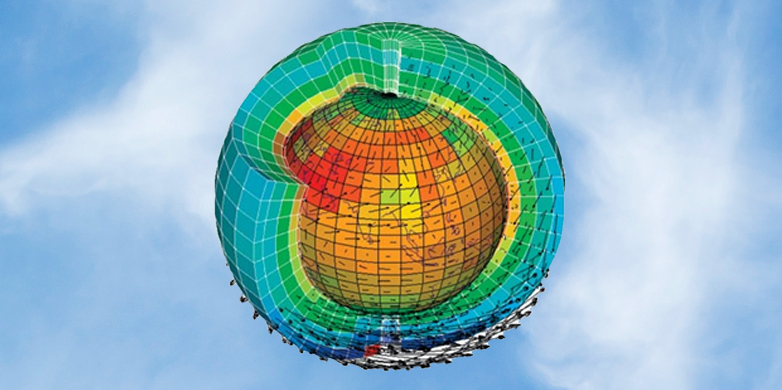
\includegraphics[width=\columnwidth]{images/weather_simulation_earth.jpg}
  \caption{ The world as a computational grid (Illustration: Carbones EU
  Project)}
  \label{fig:weather_simulation_earth}
\end{figure}

In the last part of the thesis, we experiment with the training of statistical
models on data collected from generated programs. We show that even basic
models can be trained to predict register usage accurately. Lastly, we outline
promising future research directions that can build on top of our approach. 

\paragraph{Our main contributions are as follows:}
\begin{enumerate}
  \item Implementation of the translation pass from the Standard and GPU MLIR
  dialects into a CUDA C code.
  \item A novel, random stencil program generator that replicates any set of
  stencil programs written in MLIR Stencil dialect into a variable-length set
  of new random programs that have a structure similar to the original ones.
  \item Feature extraction and optimization passes that can be used to create
  noise-free datasets suited for training of machine learning models.
  \item An accurate register prediction model trained on the generated data
  and validated on the COSMO stencils. Its prediction speed is 50 times
  faster than obtaining register usage information via \texttt{nvcc}.
\end{enumerate}

\paragraph{Thesis structure}

In Chapter~\ref{sec:Chapter2}, we discuss the theoretical background
as well as the MLIR compiler infrastructure, which is necessary for a
full understanding of the program generator. Chapter~\ref{sec:Chapter3}
introduces a random stencil program generator, which is our core contribution.
On the programs created by the generator, Chapter ~\ref{sec:Chapter4}
shows a feature extraction, their analysis, and register usage
prediction experiments together with the evaluation and future research
directions.

\section{MLIR \& Stencil dialect \label{sec:Chapter2}}

Compilers are a well-studied field in computer science with many well-known
algorithms, and applications spanning throughout multiple fields. They became
the "New Frameworks" since they provide full control in the optimization
process, which is something that frameworks cannot do. We can particularly
see these trends in web development (Angular, Babel, and TypeScript compilers),
and in Domain-Specific Languages (DSL), which have their usages in mathematics,
graphs, music, web, weather, and many more fields. DSLs make it easier to
create programs in some specific domain. Furthermore, novel and more aggressive
optimization strategies can be deployed as they take advantage of domain
knowledge. Domain-specific optimization is usually followed by the code
generation to one of the well-known general-purpose programming languages
like \texttt{C}, \texttt{C++} or \texttt{CUDA C}. Alternatively, the code
generation can target assembly language directly or use a compiler
infrastructure like LLVM \cite{llvm}. In general, DSL infrastructure creators
want to avoid doing redundant work as much as they can, and thus they translate
their optimized Intermediate Representation (IR) to some general-purpose IR
that comes with already built infrastructure. This cuts maintenance costs
and prevents reinventing the wheel. The strategy of creating only high-level
IR and reusing existing infrastructure to perform well-known optimizations
and lowerings to assemblies targeting different platforms is very common.
Good examples are languages like Swift, Rust, Julia or Objective C that build
on top of the LLVM. All of these languages have their own high-level IR which
they later lower to LLVM IR. However, this pattern forces language creators to
reinvent their own top-level IR together with accompanying infrastructure,
which leads to a repetitive reinvention of similar technology.

To tackle this problem as well as to unify the TensorFlow graph compilation
for different platforms, Lattner et al. \cite{lattner2020mlir} came with
a solution called Multi-Level Intermediate Representation (MLIR). This
state-of-the-art project is a novel approach to building maintainable,
reusable, and extensible compiler infrastructure. It is built on top of
LLVM so it takes advantage of all intermediate representation and
optimization passes by providing a lowering pass from MLIR IR to LLVM IR.
Furthermore, it allows users to reuse the LLVM and Clang types.
In this chapter, we are going to explain the components of MLIR that we
used as well as the Stencil dialect that was created using MLIR in the SPCL
lab for climate modeling.

\subsection{MLIR}
As already mentioned, MLIR is a novel approach to building a "new generation"
of compiler infrastructure. It tries to prevent reinventing of similar IRs
and optimizations by introducing building blocks that standardize the building
process. Furthermore, it provides infrastructure which is compatible with
all constructs built with the building blocks. In this subchapter, we are
going to explain the details of MLIR IR and its infrastructure, which we
use in our approach.

\subsubsection {MLIR Intermediate Representation}

The fundamental building block is \textbf{Operation} or \texttt{Op}. Every
instruction, \texttt{function} or even \texttt{module} are implemented with
use of \texttt{Op}. MLIR does not come with prebuilt operations but rather
encourages users to come up with their own. Since

\begin{figure}
  \centering
  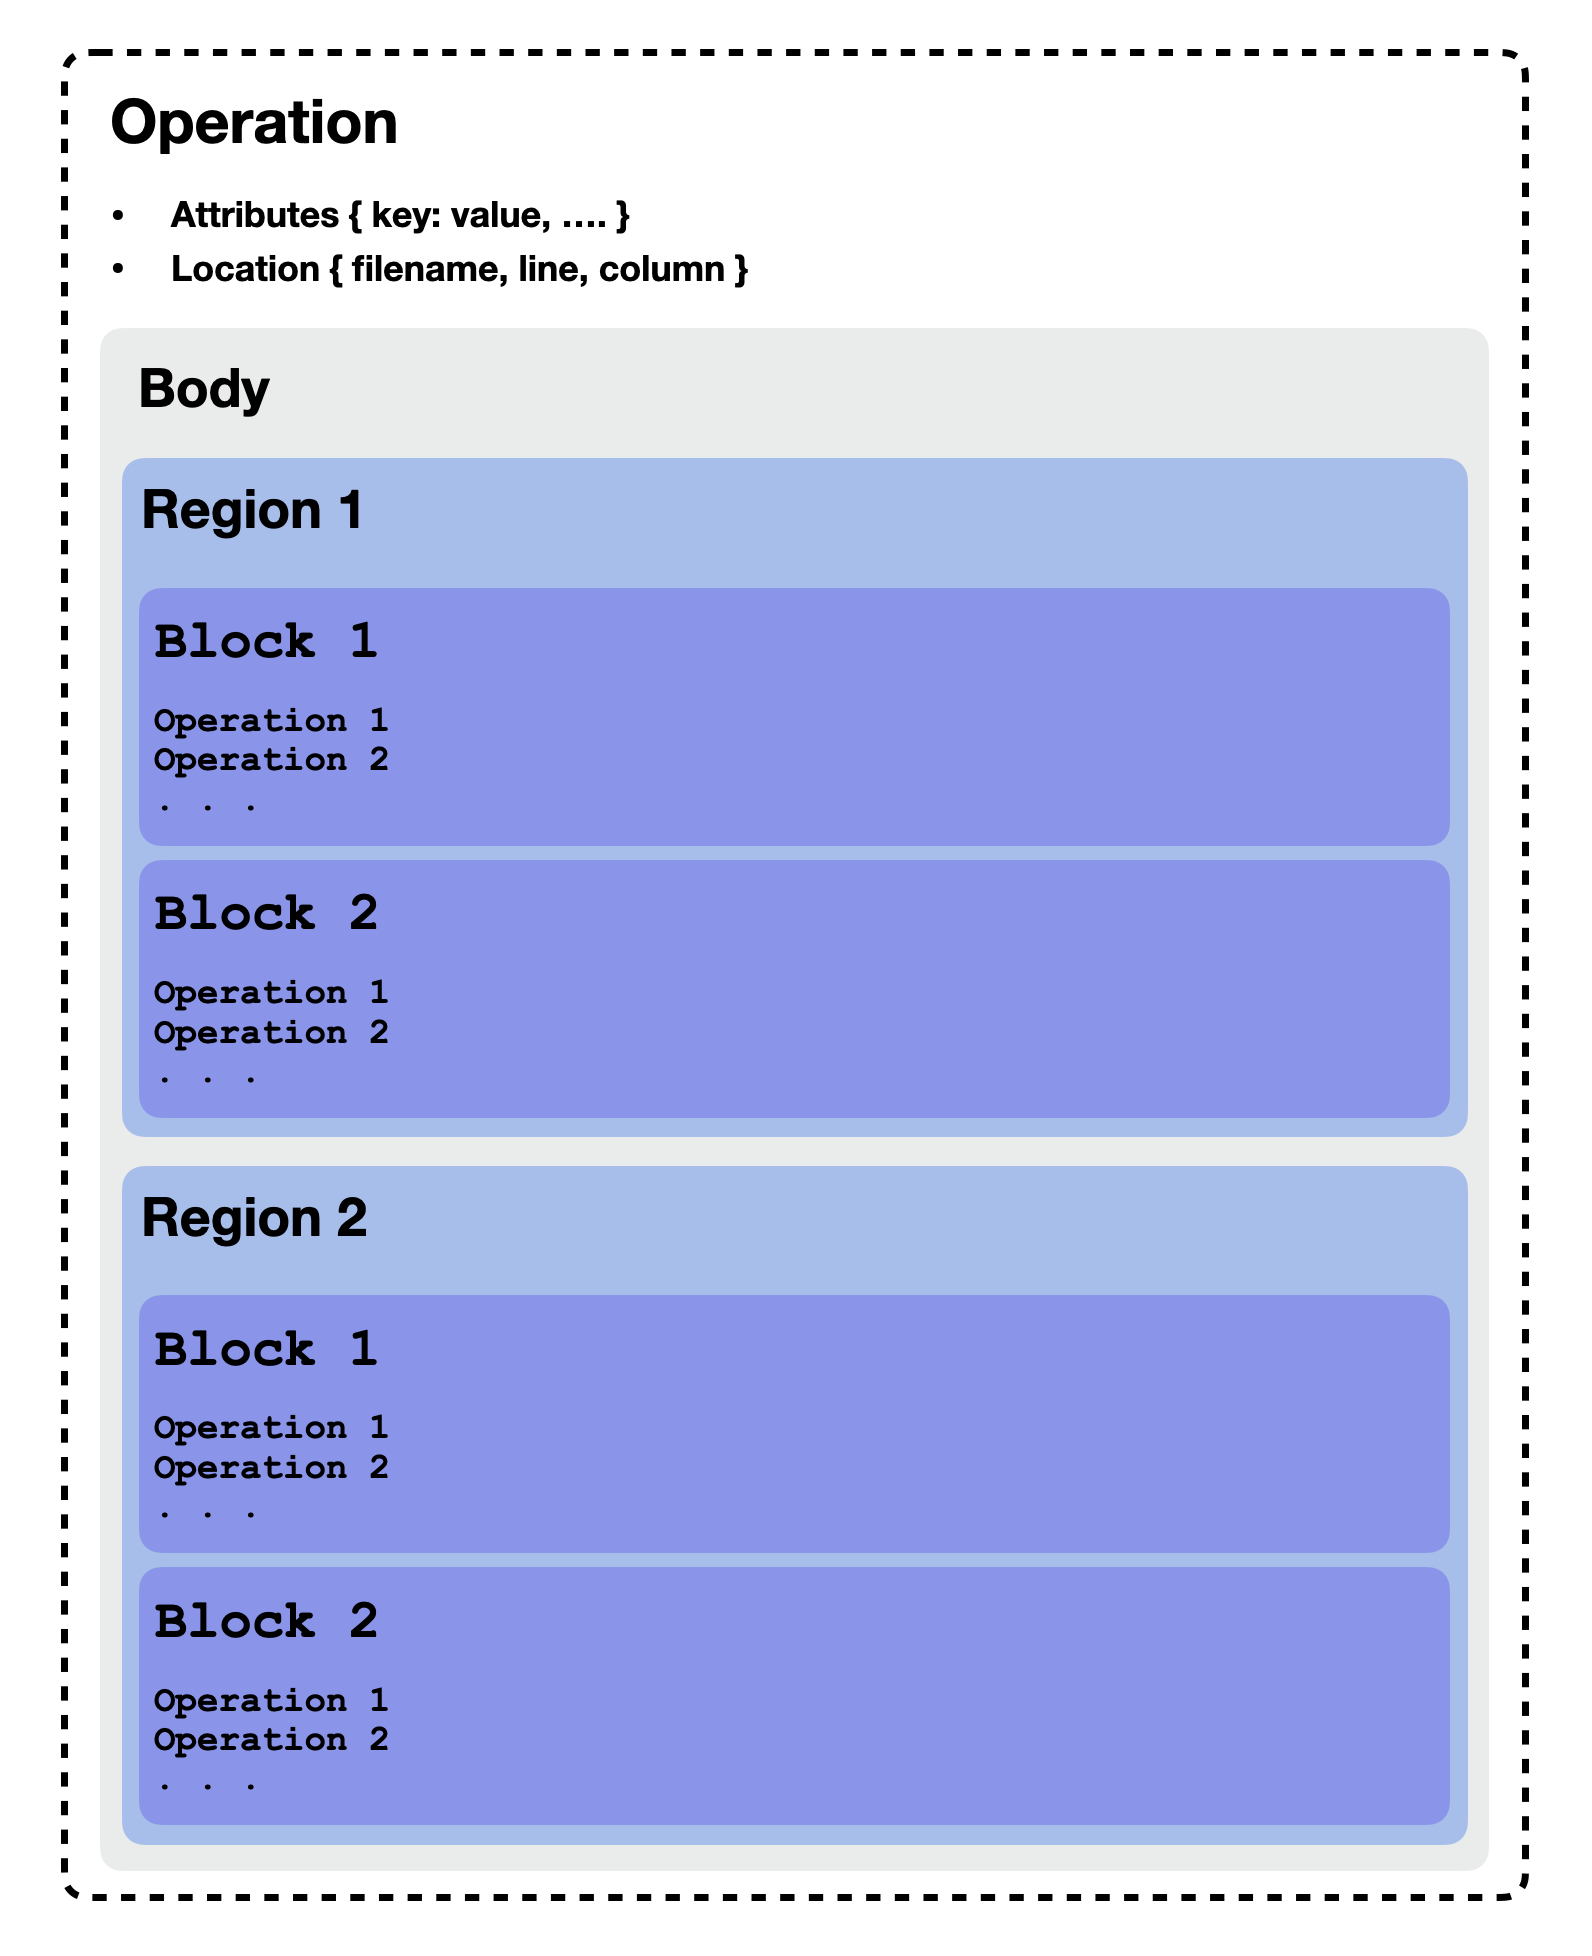
\includegraphics[width=\columnwidth]{images/operation_struct.png}
  \caption{A structure of an MLIR \texttt{Operation}. The body consists
  of zero or more regions. \texttt{Region} can have zero or more blocks.
  \texttt{Block} groups operations that are executed sequentially one after
  another.}
  \label{fig:operation_struct}
\end{figure}

\noindent every newly defined
operation inherits from \texttt{Op}, predefined compiler passes are compatible
with all operations. They are conservative but can be instructed with help of
traits, operation hooks or optimization interfaces to understand the semantics
of a new operation. Each \texttt{Op} can take zero or more values, that are
called \textit{operands}, and produce zero or more values, that are called
\textit{results}. Furthermore, it can contain \textit{Attributes},
\textit{Block Arguments} and \textit{Regions}. Every \texttt{Op} has a
\textit{Location} metadata, which describe its location in the source code.
This object is very useful in error tracing as it helps in reversed tracking.

The next MLIR construct is an \textbf{Attribute}. It provides static,
compile-time known information like constants of various types. Each operation
can contain zero or more attributes. Internally, they are represented as
key-value pairs. Therefore each attribute has to be uniquely identifiable
within an operation. Attributes are very extendible, as some attributes have
meaning only by their presence while some represent complex data structures.

Each operation inside MLIR can be uniquely identified by its \textbf{Location}.
It is strongly encouraged to forward location in between lowering passes to
keep track of the initial location in the source file, which speeds up
debugging and error identification. 

Nested structures are represented by a \textbf{Region} and a \textbf{Block}.
Each operation can have a list of the attached regions. A region contains a
list of blocks, and each block contains a list of operations where each
operation can have a list of regions. This design enables building program
structures of arbitrary depth. A region represents a Control Flow Graph (CFG)
since it contains blocks that represent straight-line code sequences terminated
by terminators, which can point to other blocks and thus form a graph. Since
MLIR IRs are in SSA form, the authors decided to replace $\Phi$ nodes with
block arguments. Each terminator can point to another block with a different
argument and thus avoid a need for the $\Phi$ node.

MLIR operations are grouped in \textbf{functions} and \textbf{modules}. An
MLIR function is very similar to a C function. It can take zero or more
arguments, but it can also produce zero or more results. A function is thus
a constrained operation since it has only one region with one block as it
has only one body. The terminator of a function is return operation, which
returns whatever is passed as its operands. Similarly, a module is an operation
with one region containing one block, which can have an arbitrary number of
other types of operations. A module is terminated by a special, dead-end module
terminator which does not transfer control flow any further.

MLIR offers extensibility via \textbf{Dialects}. A dialect is a namespace that
groups together attributes, types, and operations. Dialect name appears
dot-separated before each operation from the dialect, which provides a visual
grouping of its operations and improves a readability of the code. Dialect's
main purpose is a logical grouping of operations, but it can provide some
generic operation functionalities as well. Users are not forced to use some
predefined patterns for dialects, but they are given freedom in their usage.
However, as with namespaces, it is recommended to group the operations within
the same project to a dialect not only for readability purposes but also to
prevent the naming collisions. A good example would be use of \texttt{Vector},
\texttt{Load} or \texttt{Store} names for operations. These names already exist
in the standard dialect and thus are always prefixed with \texttt{std}. If
users want to define their operation with one of these names, they will
encounter no conflicts as each operation will be prefixed with a different
dialect name.

\begin{figure}
  \centering
  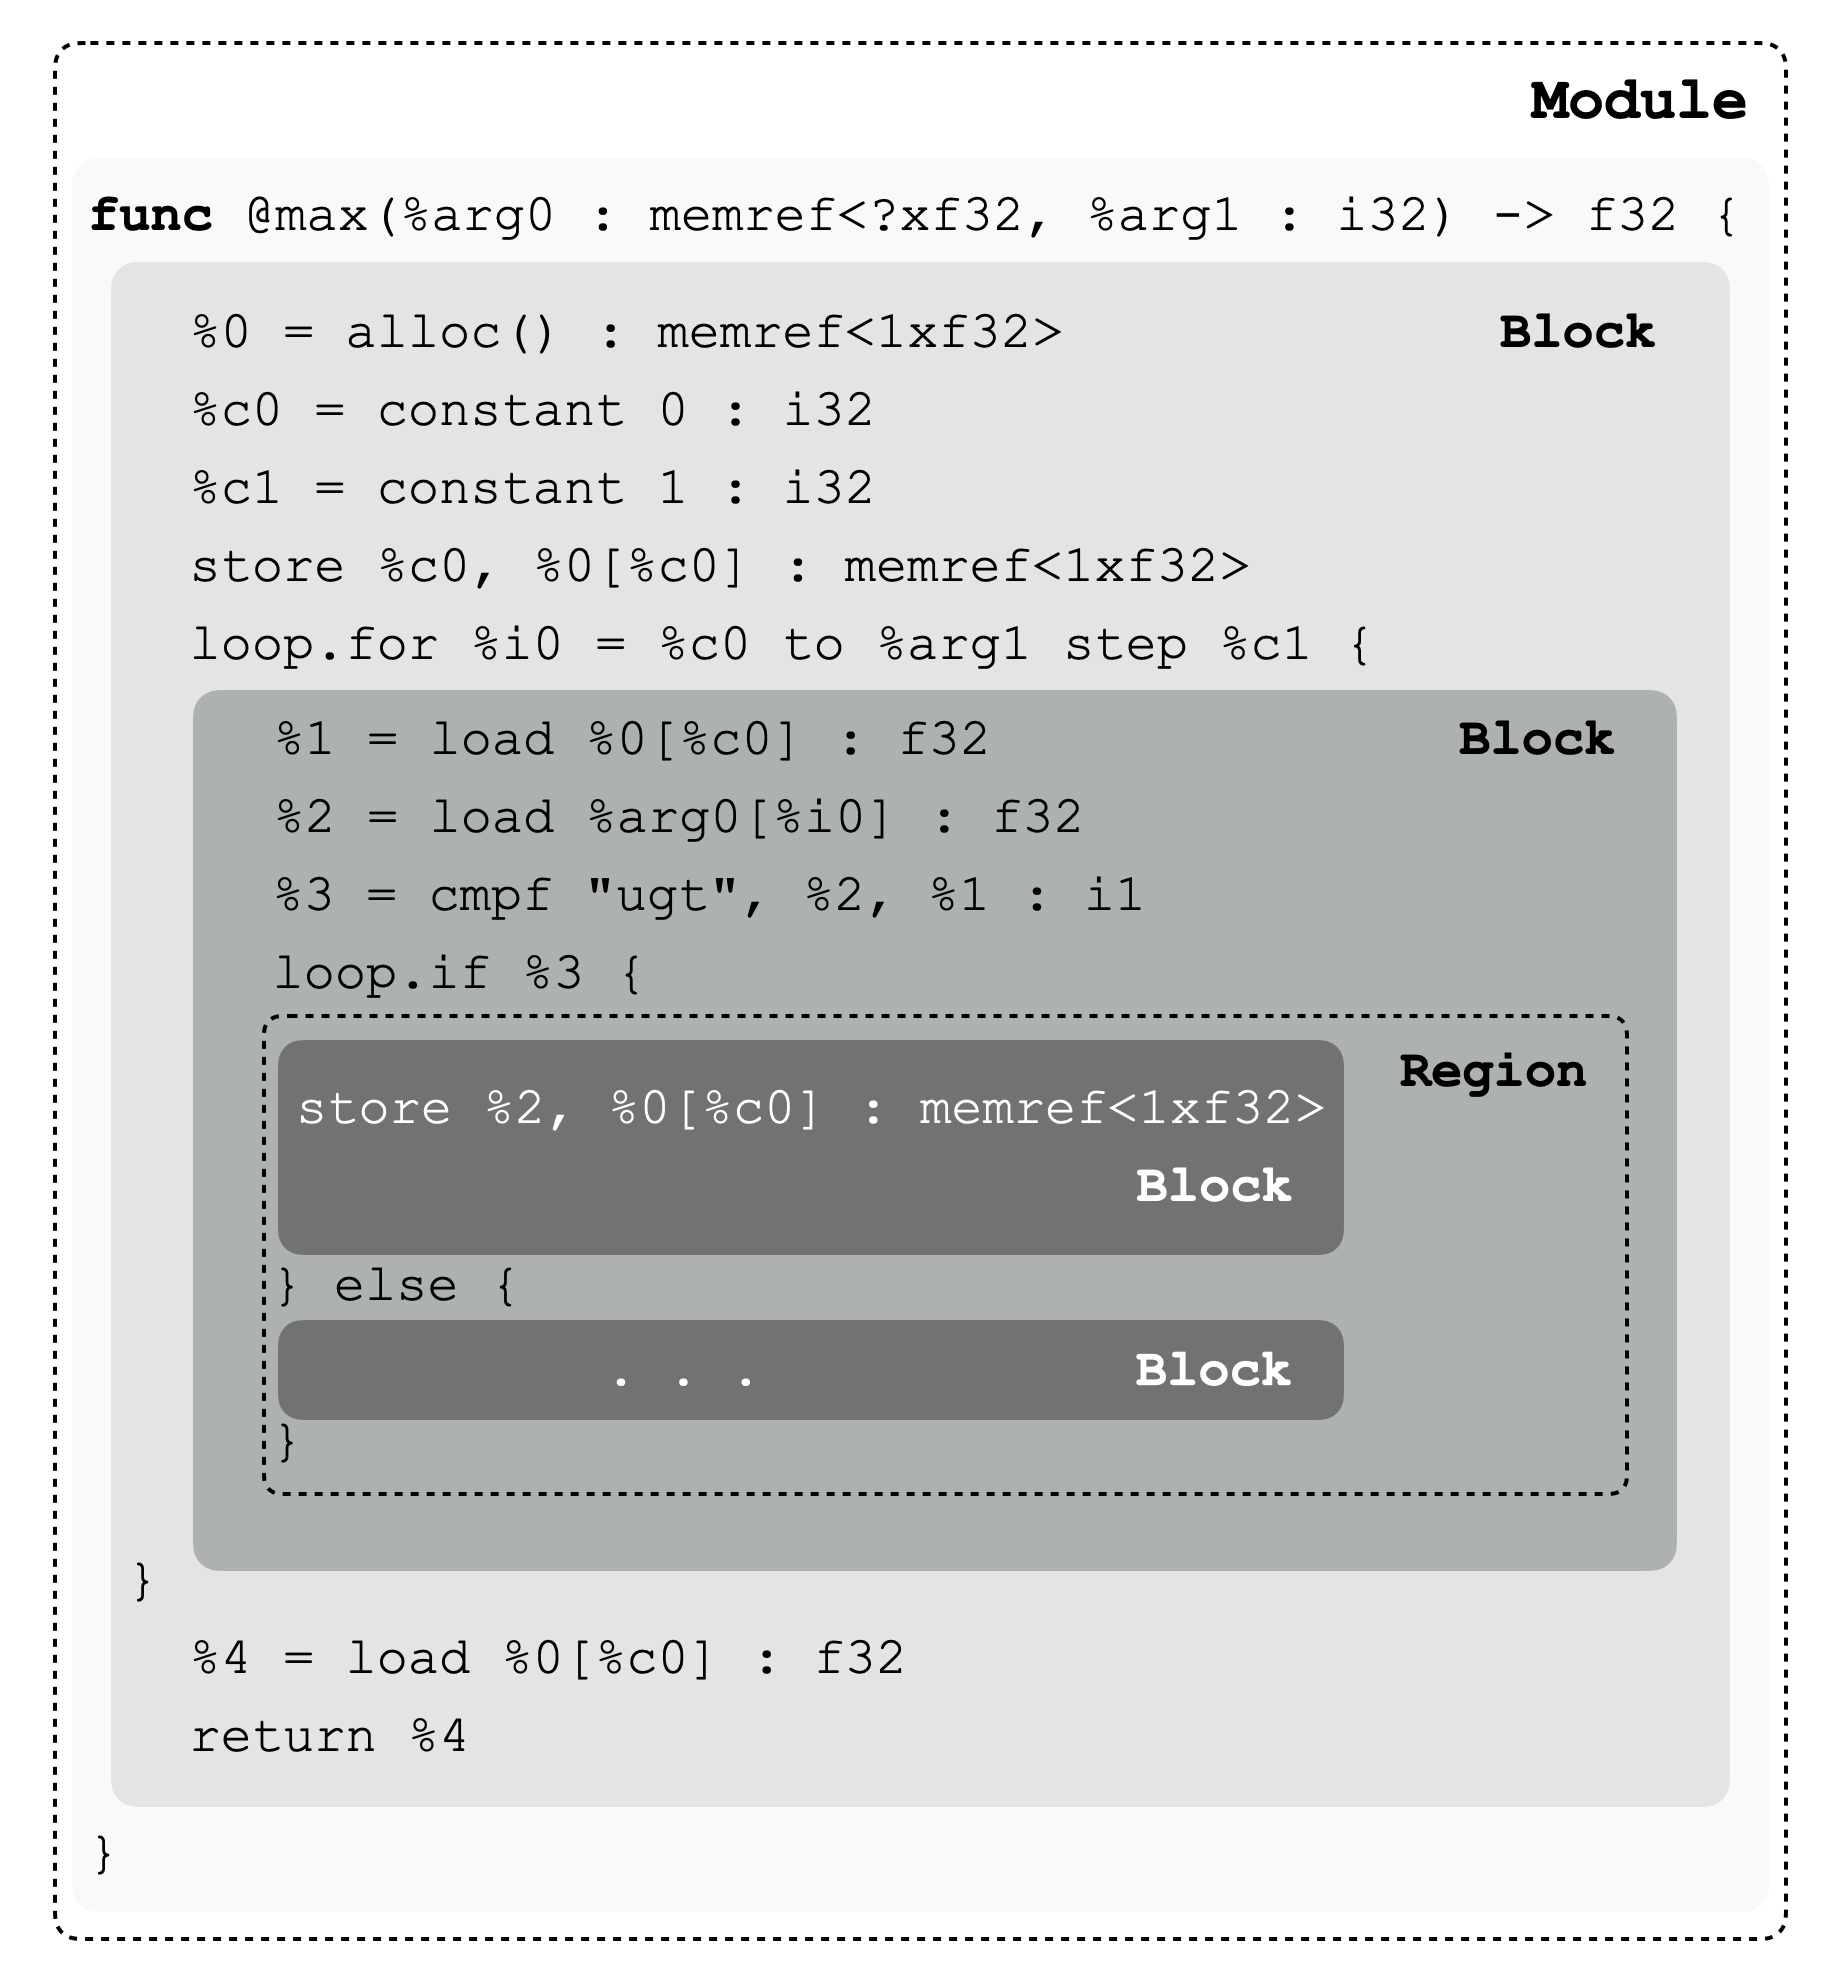
\includegraphics[width=\columnwidth]{images/mlir_max.png}
  \caption{The figure shows a function returning maximal element from an array
  passed as an argument together with its size. The function is wrapped in the
  \texttt{Module} operation, which is always a top-level parent operation. A
  body of a function is represented as a \texttt{Block} of operations. Some
  \texttt{Operations} like \texttt{loop.if} can have a body and thus their
  attached list of regions is not empty.}
  \label{fig:mlir_max}
\end{figure}

Users do not need to be reluctant in introducing more dialects due to
compatibility issues, as MLIR allows mixing of dialects. Distinct dialects can
coexist at any level and at any time in the IR. For instance, in our approach,
we mix our custom dialect with the standard one, so we do not need to redefine
all standard arithmetic operations. Furthermore, we use a \texttt{loop.if}
operation from the loop dialect for branching.

The last important part of MLIR is a \textbf{type system}. Every value has to
have a type. MLIR comes with a predefined set of types -
\textbf{Standard Types}, like floats and integers of various bit lengths,
pointers or memory references. However, users can define their types inside
dialects as well. Furthermore, types from existing systems (LLVM, Clang) can
be used. They need to be prefixed with llvm or clang namespace respectively
i.e. \texttt{llvm::SmallVector} or \texttt{clang::math::min}.

\begin{figure}
  \centering
  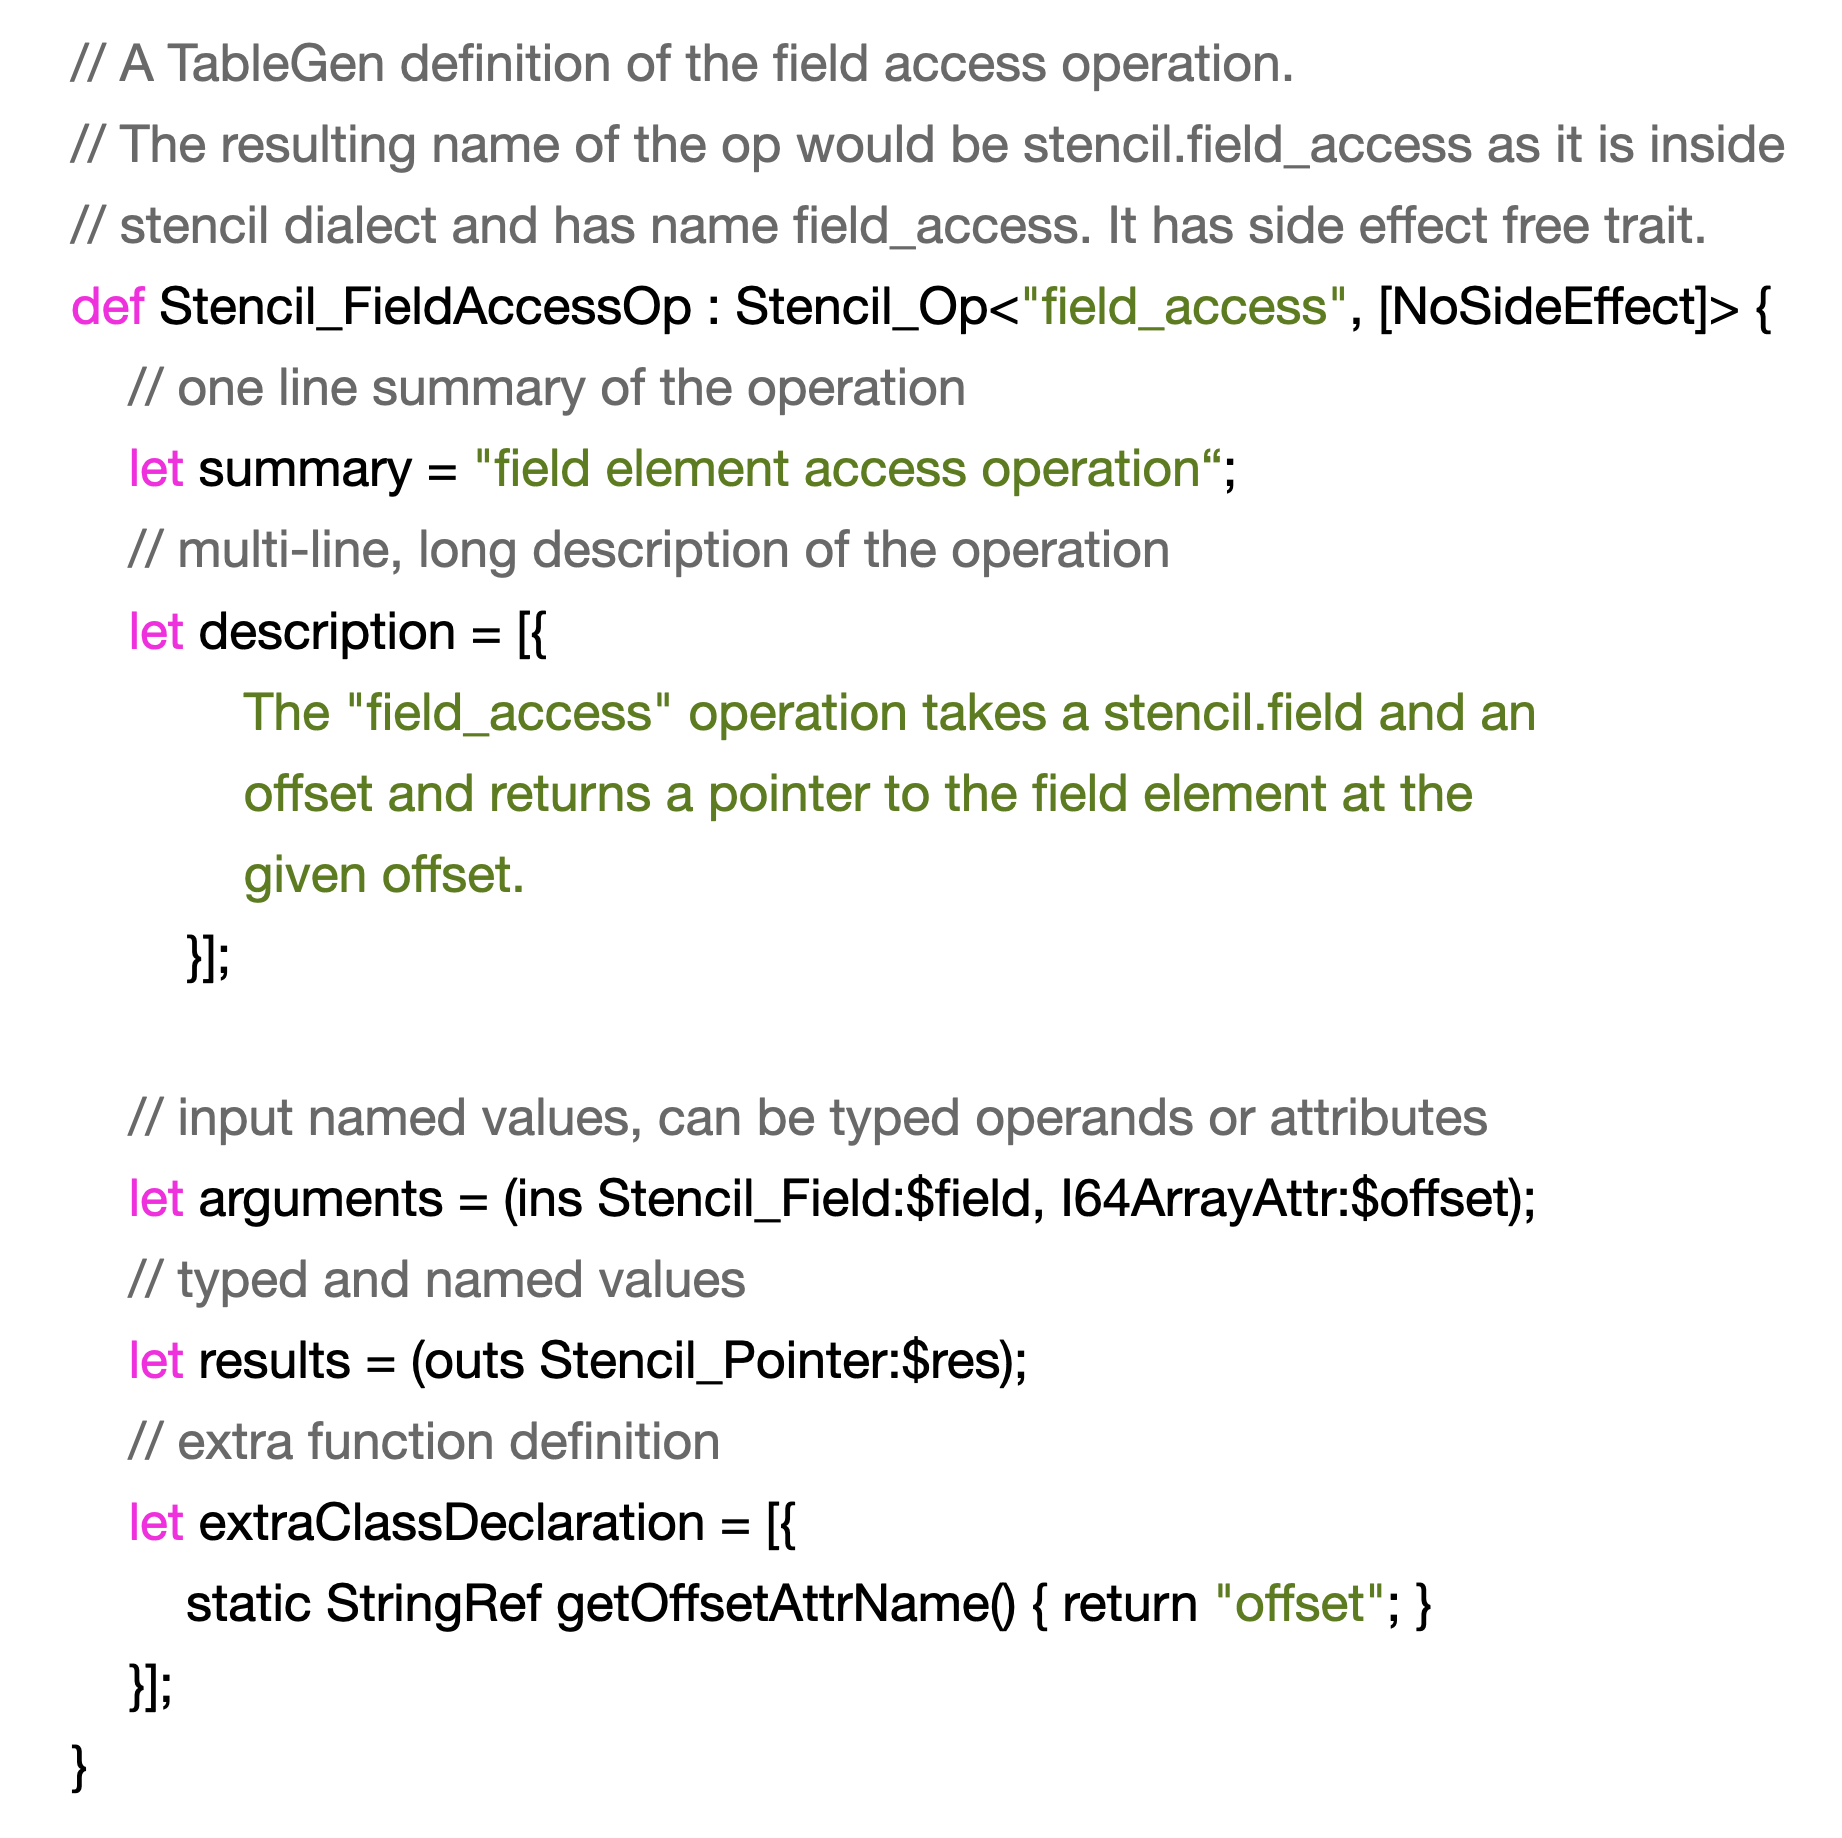
\includegraphics[width=\columnwidth]{images/op_definition.png}
  \caption{An example of Operation Definition Syntax (ODS), which is the 
  way of defining new operations in MLIR. This example shows a shortened
  definition of the \texttt{FieldAccessOp} that is a fundamental operation
  in the Stencil dialect.}
  \label{fig:op_definition}
\end{figure}

\subsubsection{MLIR Passes and Op Definitions}
MLIR consists of two main components. An IR, which we already described and
IR infrastructure, which parts we are going to describe in this subchapter.

New operations are created in MLIR with specifications, which are based on
TableGen \cite{tablegen} and are called Operation Definition Syntax (ODS).
This syntax reduces the amount of boilerplate code that needs to be written
by allowing user to write only essential parts of the operation like
\textit{summary}, \textit{description}, \textit{arguments}, \textit{results},
\textit{builders} or \textit{verification} method. Furthermore, user can
specify traits which are helpful for passes to understand the semantics of
an operation. For instance, \texttt{[NoSideEffect]} trait tells optimization
passes that the operation is side effect free. The real \texttt{C++} classes
are table generated during the compilation. An example of the
\texttt{FieldAccessOp} definition can be seen in figure
\ref{fig:op_definition}.

MLIR IR is being processed with passes. A pass takes an IR as an input and
produces transformed IR as an output. In theory, 2 types of transformations
can be applied. The first one optimizes the given IR, and the second one
lowers it. Practically, MLIR does not distinguish between these two types.
It only verifies that transformations produce valid IRs. Therefore it is up
to users how they want to structure passes. Furthermore, MLIR provides a pass
infrastructure - pass manager, which manages the series of IR passes. MLIR
provides 3 types of IR traversals. 

\begin{itemize}
  \item \textbf{ModulePass} runs on every module in an IR. The user implements
  a callback function, which is supposed to handle each module.

  \item \textbf{FunctionPass} runs on every function, users have to implement
  a callback function to handle each MLIR function.

  \item \textbf{OperationPass} Runs on every operation. Users can narrow down
  the type of iterating operations. However, this pass does not allow any
  parent or parent region to be modified, only the currently iterated operation
  and its children.
\end{itemize}

Users create passes to do the transformations, which require a lot of operation
rewriting. MLIR has a solution for that in the form of rewriters, conversion
patterns, and type converters. Conversion patterns match and rewrite operations
specified by a user. An operation match consists of an operation type match and
a user-provided condition. Furthermore, MLIR comes with a generic, predefined
passes. These passes provide either conversion between MLIR dialects or
optimizations like Common Subexpression Elimination (CSE) or Canonicalization.
All predefined optimizations are generic enough to handle new, properly
annotated operations. Annotation with traits is required for them to work well
as they give semantics information.

\subsection{Stencil Dialect}
In this subchapter, we are going to first introduce stencil computations for
weather modeling followed by the Stencil dialect \cite{jmgorius1},
\cite{jmgorius2} written by Jean-Michel Gorius during his research internship
at ETH Zurich, which represents them in MLIR dialect. Our coverage of these
topics is far from being comprehensive as it aims to give the reader sufficient
information to understand the topics that follow. For more detailed information
one can follow up here \cite{Roth97compilingstencils}, \cite{Holewinski},
\cite{jmgorius1}, \cite{jmgorius2}.

\subsubsection{Stencil Computations}

A stencil kernel is a type of computational kernels, which iteratively
traverses a grid and updates each cell based on the adjacent cells.
The pattern in which adjacent cells are accessed is called \textit{stencil}.
Such stencil can be executed on regular \cite{bianco2012generic} and irregular
\cite{irregular} grids. A regular grid is represented as 2D or 3D array
depending on the space in which a stencil is computed. In our approach, we
do not consider irregular grids.

A typical usage of stencil computations is in weather simulations where
grids are initialized with the current weather situation and the stencil kernel
is iteratively run on the grid to simulate the change of the weather elements
like temperature (heat and cold diffusion) or humidity. The iteration method
is called \textit{Jacobi method} \cite{jacobi}, which iteratively solves a
strictly diagonally dominant system \cite{diagonal_matrix} of linear equations
\cite{linear_eq}. For example, a following second-order partial differential
equation:
\begin{equation}
\frac{\partial^2 F}{\partial x^2} + \frac{\partial^2 F}{\partial y^2} = 0
\end{equation}
\noindent is solved iteratively on grid $G$ as:
\begin{equation}
  G_{new}(i,j) = \frac{1}{4}(G(i-1,j) + G(i+1,j) + G(i,j-1) + G(i,j+1))
\end{equation}
\noindent i.e. by taking average of all 4 neighbouring cells. In another
words, each cell is in each iteration equally influenced by all its neighbours.
For instance, this is very useful in modelling of heat diffusion as heat
spreads out through the space by heat transfer from one particle to another.

Our research area is to not come up with new stencil computations but to
support the scientists working on them with high performance and user-friendly
execution infrastructure.

\subsubsection{Dialect Definition}

In this subchapter, we are going to describe each operation inside the MLIR
Stencil dialect. However, we are not its authors. Therefore we will not reason
about design decisions. The goal of this subchapter is to give the reader a
short reference as the next chapter builds heavily on that knowledge.

As shown in figure \ref{fig:pipeline_lowering} an input to the Stencil compiler
is a stencil file exported from \texttt{Dawn} \cite{dawn} compiler. The
authors created an intermediate dialect called IIR to model \texttt{dawn}
format inside MLIR because each dialect can specify parse methods that lead
the MLIR parser in parsing input files. Therefore, the sole purpose of the IIR
dialect is to parse stencils exported from the \texttt{dawn}. It is always
subsequently lowered into the Stencil dialect. 

Stencil dialect tries to leverage existing MLIR IR by introducing types and
operations that do not occur in MLIR. Thus it reuses standard arithmetic
operations and types like additions, multiplications, or floats. It
introduces only the following types:
\begin{itemize}
  \item \textbf{FieldType} \texttt{!stencil<"field:f64">} represents a
  reference to a grid, which can be called \textit{field} as well. In
  the current stage of dialect development we support only 3 dimensional grids.
  \item \textbf{VarType} \texttt{!stencil<"var:f64">} represents a stencil
  variable, that acts as a normal variable and is shared between
  DoMethods in the same Stage.
  \item \textbf{PointerType} \texttt{!stencil<"ptr:f64">} A pointer to
  a stencil field. Can be dereferenced to get the value and written to.
\end{itemize}

The only type used from the standard types is \textit{f64}, which represents a
value in each cell of the grid as well as the result of the comparison.
The following operations form an IR structure of the stencils. Most of them
are omitted in the lowering passes as they do not influence the computations:

\begin{itemize}
  \item \textbf{IIROp} \texttt{stencil.iir(StrAttr:\$stencilName)} groups
  multiple stencils.
  \item \textbf{IIREndOp} \texttt{stencil.\_iir\_end} terminates an IIROp. 
  \item \textbf{StencilOp} \texttt{stencil.stencil} Represents a stencil
  computation. It can contain various stencil kernels located in multiple
  stages and multi-stages. Takes zero or more fields (grids) as arguments.
  Stencil does not distinguish between input and output fields. All fields
  can be read and written.
  \item \textbf{StencilEndOp} \texttt{stencil.\_stencil\_end} terminates
  a StencilOp.
  \item \textbf{MultiStageOp} \texttt{stencil.multi\_stage} groups multiple
  Stages. Has one mandatory parameter - an order in which stages are executed.
  The order can take these values: \textit{Forward}, \textit{Backward},
  \textit{Parallel}.
  \item \textbf{MultiStageEndOp} \texttt{stencil.\_multi\_stage\_end}
  terminates a MultiStageOp.
  \item \textbf{StageOp} \texttt{stencil.stage} groups multiple DoMethods.
  \item \textbf{StageEndOp} \texttt{stencil.\_stage\_end} terminates
  a StageOp.
  \item \textbf{DoMethodOp} \texttt{stencil.do\_method} DoMethod represents
  a stencil kernel. It groups arithmetic, read, and write operations that do
  the actual computation. Takes 4 static parameters of integer type that
  specify lower bound, lower offset, upper bound, and upper offset on the
  kernel iterations.
  \item \textbf{DoMethodEndOp} \texttt{stencil.\_do\_method\_end} terminates
  a DoMethodOp.
\end{itemize}

\begin{figure}
  \centering
  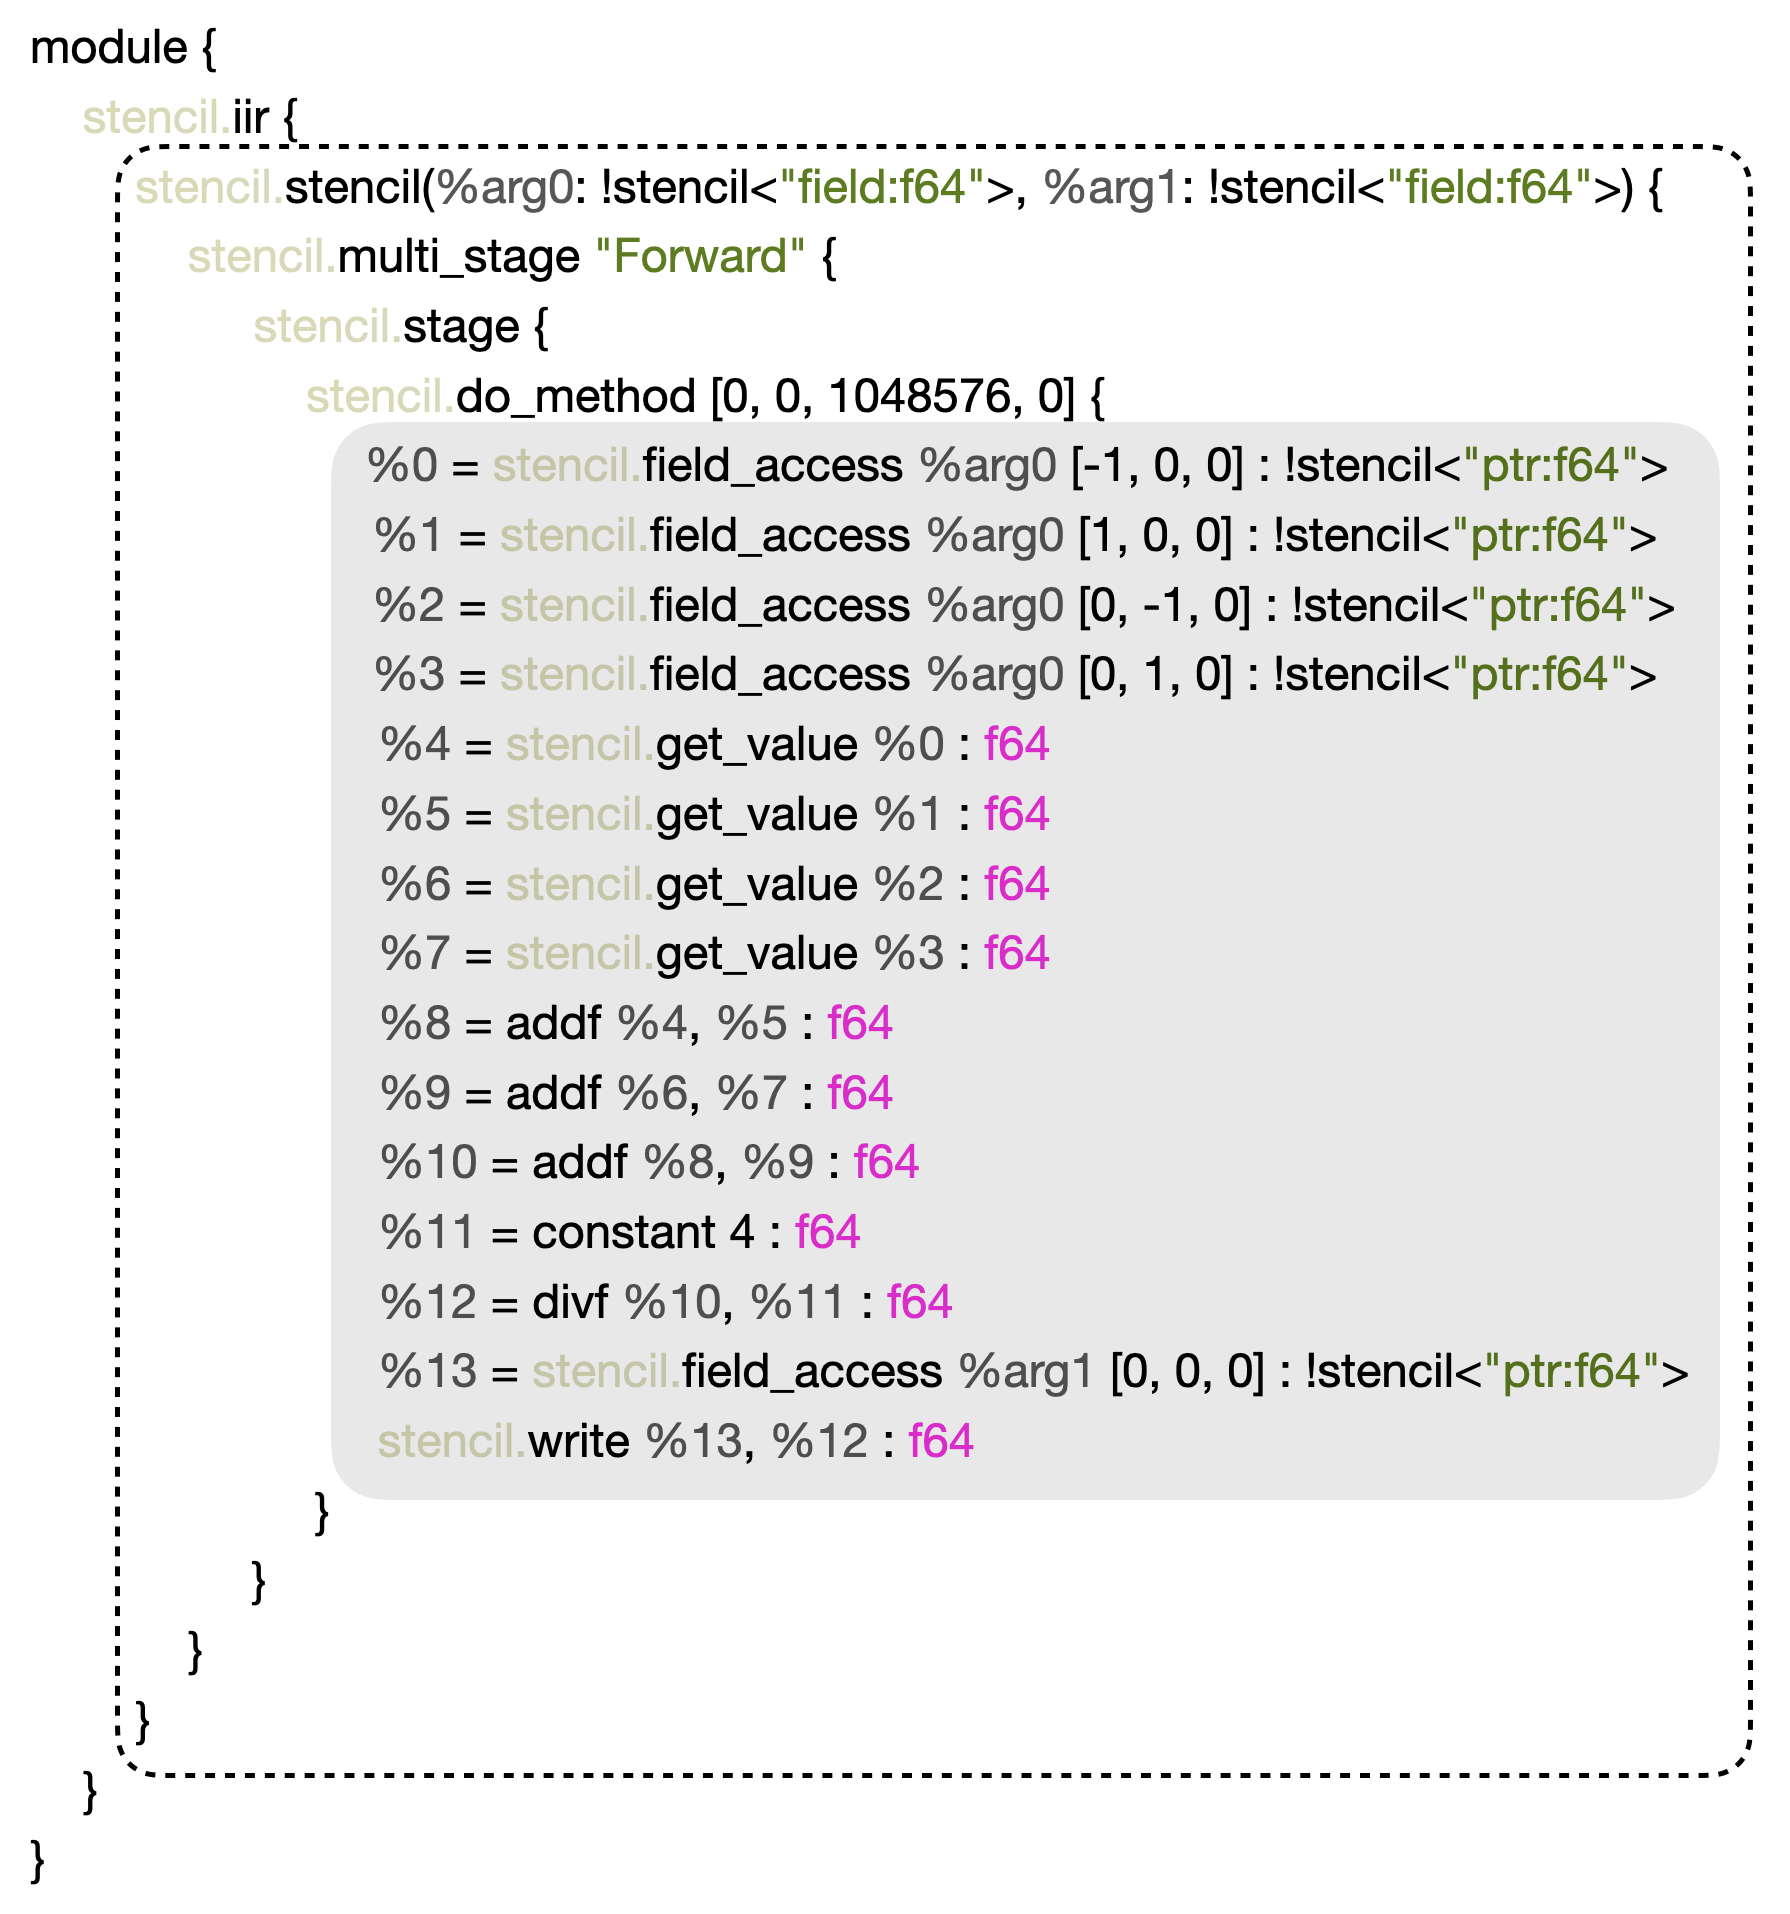
\includegraphics[width=\columnwidth]{images/jacobi_stencil.png}
  \caption{Jacobi stencil implemented in the Stencil dialect.
  The dashed line marks the actual stencil while the gray box
  highlights the body of the DoMethod.}
  \label{fig:jacobi_stencil}
\end{figure}

The second group of stencil operations consists of operations that occur
inside DoMethod. The only exceptions are \textit{FieldOp} and \textit{VarOp},
which are located outside of it. The full signature of each operation can be
found in the appendix. \textit{SqrtfOp}, \textit{FabsOp}, \textit{ExpOp},
\textit{PowOp} were added as the standard dialect does not support them.

\begin{itemize}
  \item \textbf{FieldOp} \texttt{stencil.field} Allocates memory for a local
  field and returns a reference to it.
  \item \textbf{FieldAccessOp} \texttt{stencil.field\_access} Takes a field
  and a 3 dimensional offset as an input, produces a field pointer.
  \item \textbf{VarOp} \texttt{stencil.var} Creates a local variable.
  \item \textbf{VarAccessOp} \texttt{stencil.var\_access} Takes a variable
  as an input and returns a pointer pointing to it.
  \item \textbf{GetValueOp} \texttt{stencil.get\_value} Dereferences a pointer
  passed as an argument. Returns the scalar located at the corresponding memory
  address.
  \item \textbf{WriteOp} \texttt{stencil.write} Writes a scalar to a pointer.
  Both of them are passed as arguments.
  \item \textbf{SqrtfOp} \texttt{stencil.sqrtf} Computes the square root of a
  floating-point number.
  \item \textbf{FabsOp} \texttt{stencil.fabs} Computes the absolute value of
  a floating-point number.
  \item \textbf{ExpOp} \texttt{stencil.exp} Computes the value of the
  exponential of a floating-point number.
  \item \textbf{PowOp} \texttt{stencil.pow} Computes the floating-point power
  of two numbers.
\end{itemize}

\noindent An example of \texttt{Jacobi stencil} in the Stencil dialect can be
seen in figure \ref{fig:jacobi_stencil}. The example demonstrates the usage of
the operations described above. The computation itself happens inside the body
of DoMethod, where all adjacent cells are read, their average is computed and
stored to the output stencil. 

\subsubsection{Lowering Pipeline}
So far, we have a working Stencil dialect and a way of transforming
\texttt{dawn} files into it. Since our goal is to execute stencils on the GPU,
the next step is to translate a program from the Stencil dialect to CUDA C.
Therefore, a lowering pass to the mix of affine and standard dialect was
created to reuse the existing MLIR passes for lowering affine dialect to the
GPU one. This conversion automatically creates a Cuda kernel together with a
launch function. The last step in the conversion is to translate the mix of
GPU and standard dialect into Cuda C. Here lies our first contribution as we
implemented this conversion. The stencil is run by:
\begin{enumerate}
  \item creating a file with the main function, where all grids are initialized
  \item linking generated CUDA C file
  \item calling the launch function with the initialized grids
  \item compiling both of them with \texttt{nvcc}
  \item running generated executable.
\end{enumerate}

\begin{figure}
  \centering
  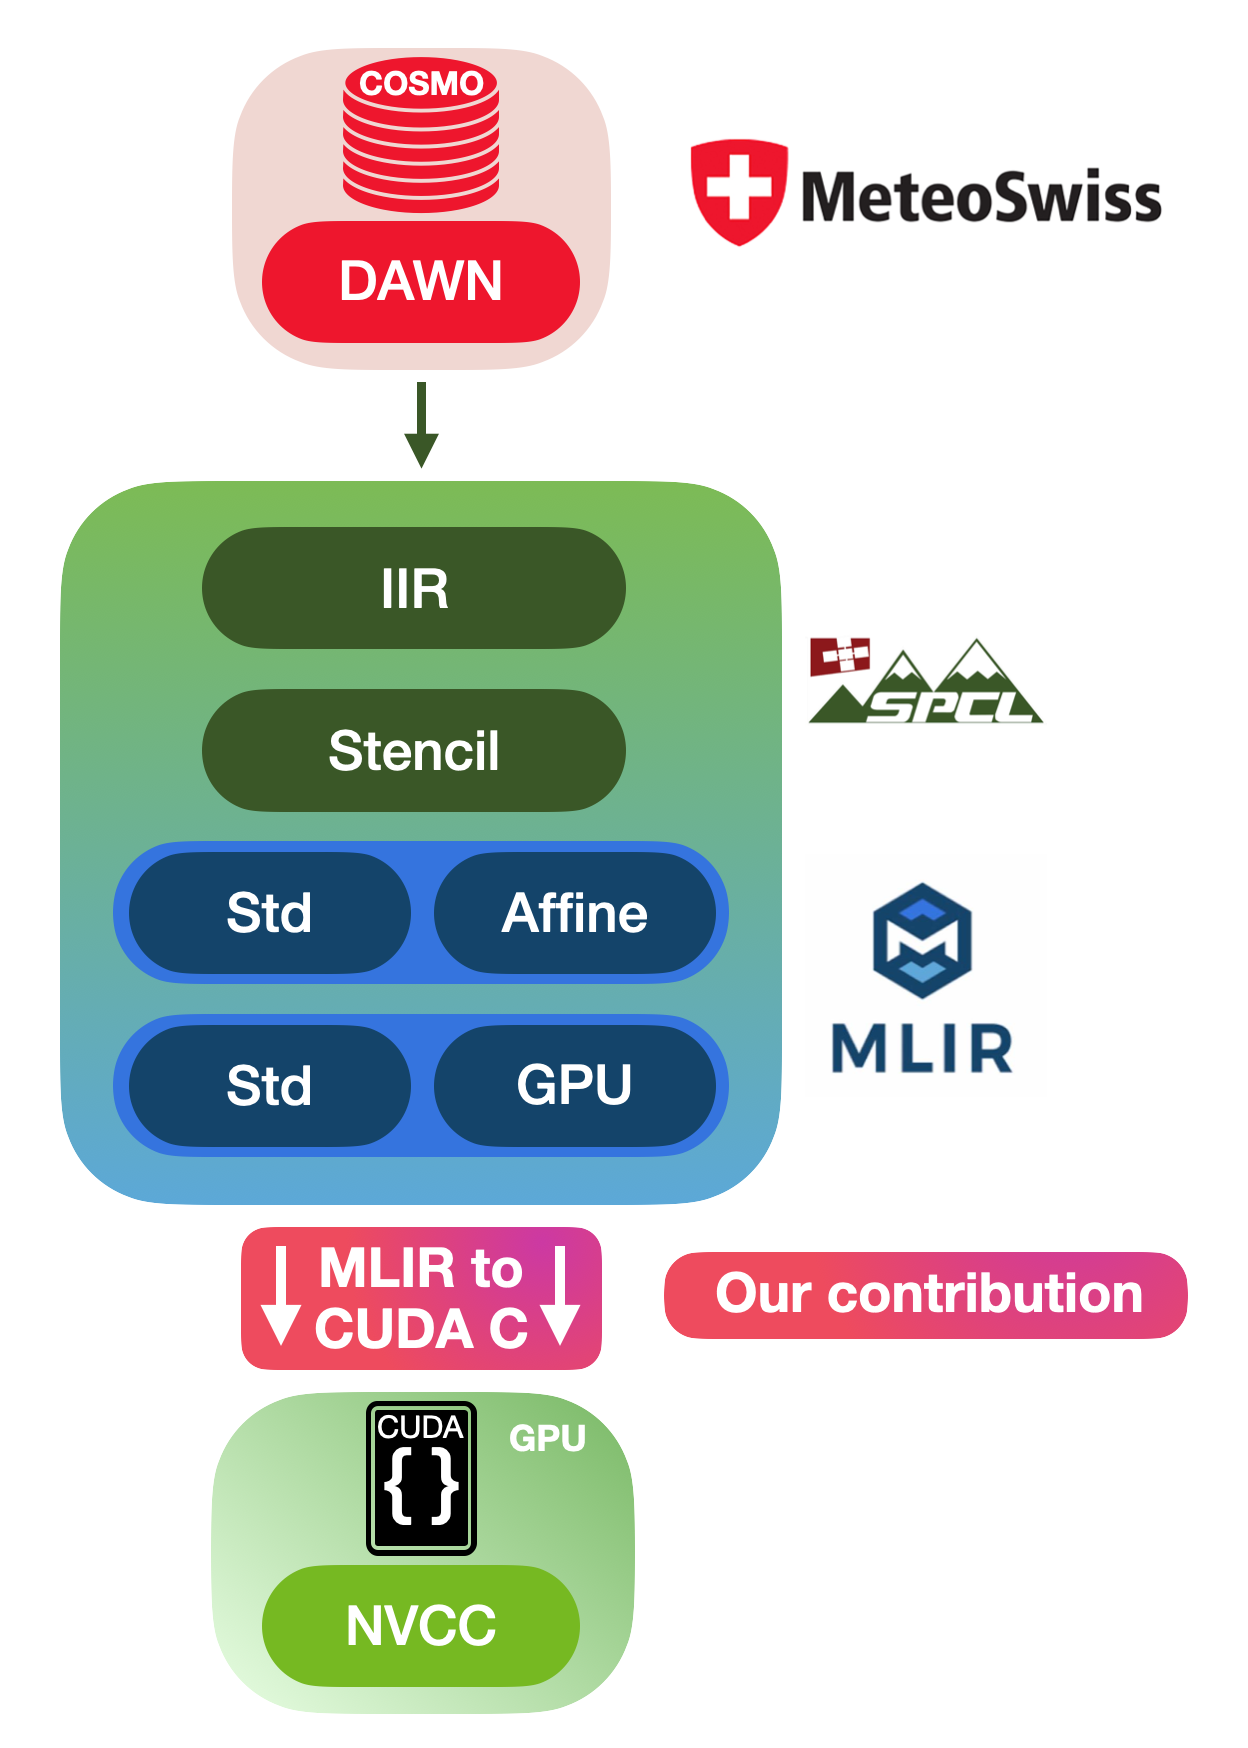
\includegraphics[width=0.9\columnwidth]{images/lowering_pipeline.png}
  \caption{Current pipeline of the Stencil compiler. The input
  consists of COSMO stencils exported from the \texttt{dawn} compiler.
  Consequently, MLIR Stencil compiler loads and lowers them to the GPU dialect.
  Our contribution consists of translating the resulting mix of GPU and
  standard dialect into CUDA C code, which is compiled by the \texttt{nvcc}
  an executed on Nvidia GPU.}
  \label{fig:pipeline_lowering}
\end{figure}

\section{Random Stencil Program Generator \label{sec:Chapter3}}

The generation of meaningful random programs is a well-studied field in
computer science. Random programs complement human-written ones in compiler
testing as they can provide execution patterns that compiler creators were not
considering. Moreover, they can act as compiler fuzzers that exhaustively test
compilers for errors such as segmentation faults or floating-point errors.
Lastly, they can be time-savers for the testers as they are capable of much
faster program generation than humans. However, our goal is not to use the
generator for compiler correctness even though it can be used for that as
well. We need it for enlarging the stencil dataset as the COSMO model contains
only around 30 stencils, which are not sufficient for the training of any
model. Therefore the most desired properties of our generator are the quality
and variety as we want to generate programs that look like they were written
by a human but novel in some sense as well. In this chapter, we are going to
introduce the "guts" of our random stencil generator as well as some more
high-level concepts it builds on. 

\subsection{Generation Pipeline}
Rather than generating a program in a single pass, we decided to make it a
little bit modular and split it into two passes. The first one, which we call
program chain generation, takes a set of valid stencil programs as an input
and generates an operation chain without any arguments or return values. The
chain defines an order in which one operation follows another in the source
file. An example of such a generated chain can be:\\\\
\label{chain}
\texttt{module} $\rightarrow$
\texttt{iir} $\rightarrow$
\texttt{stencil} $\rightarrow$
\texttt{multi\_stage} $\rightarrow$
\texttt{stage} $\rightarrow$
\texttt{do\_method} $\rightarrow$ \\
\texttt{field\_access} $\rightarrow$
\texttt{field\_access} $\rightarrow$
\texttt{get\_value} $\rightarrow$
\texttt{get\_value} $\rightarrow$
\texttt{addf} $\rightarrow$
\texttt{write} $\rightarrow$
\texttt{\_do\_method\_end} $\rightarrow$
\texttt{\_stage\_end} $\rightarrow$
\texttt{\_multi\_stage\_end} $\rightarrow$
\texttt{\_stencil\_end} $\rightarrow$
\texttt{\_iir\_end} $\rightarrow$
\texttt{module\_terminator}\\

\noindent The second phase takes the chain generated by the first phase as
an input and produces an MLIR program in the Stencil dialect.
One of many possible programs generated from the chain above could be:

\begin{lstlisting}[caption={An example of the program generated 
  from the chain},captionpos=b\label{lst:sample}]
module {
  stencil.iir {
    stencil.stencil(%arg0: !stencil<"field:f64">,
      %arg1: !stencil<"field:f64">) {
      stencil.multi_stage "Forward" {
        stencil.stage {
          stencil.do_method [0, 0, 1048576, 0] {
            %0 = stencil.field_access %arg0 [0, 0, 0]
              : !stencil<"ptr:f64">
            %1 = stencil.field_access %arg1 [0, 0, 0]
              : !stencil<"ptr:f64">
            %2 = stencil.get_value %0 : f64
            %3 = stencil.get_value %1 : f64
            %4 = addf %3, %2 : f64
            stencil.write %1, %4 : f64
          }
        }
      }
    }
  } attributes {stencilName = "addition"}
}
\end{lstlisting}

In the following subchapters, we are going to explain both phases in detail
as well as the evaluation of programs generated by them.

\subsection{Learning the Markov Chain}
Every program generator needs to understand the program structure to generate
a meaningful random program. By that, we mean, for instance, an order in which
operations follow each other, counts of operation types in the program, or
distribution of the program length. The understanding of the program structure
can be achieved either by first studying the structure and later hard-coding
it in the generator or by providing enough examples to the generator and
letting it statistically learn the structure. We decided to go for the second
option as we aim to make the generator generic enough in handling new program
structures as well as not constraining randomness by hard coding parts of it.

We can represent a structure of any stencil program as a chain of operation
types. Some of them can contain nested operations grouped in the blocks. An
example of such operation type would be the \texttt{If} operation, which has
two \texttt{Blocks} - one that is executed when the condition is evaluated to
\texttt{true} and the second one otherwise. We create chain out of nested
operations by traversing them preorder. However, they introduce chain
ambiguity as it is unclear to which parent does an operation belong. Therefore
we need to explicitly mark the end of the operation's body to know that the
following operations belong to the parent that is one level up. We achieved
that by introducing a matching body end terminator for every operation that
can have a body, as can be seen \hyperref[chain]{here}.

In this phase, we simplified our general setting only to types of operations.
We do not consider their results nor their parameters. With this setting, we
can represent the structure of a general stencil program as a Markov chain
where the state is a type of operation, and the edge from node A to node B
is a probability with which operation B follows operation A. All outgoing
edges have to sum up to 1 as they are a probability distribution of the
state. The advantage of this model is its simplicity and universality. It
is generic enough to express any program with such a structure yet very
simple to understand and train. 

\begin{figure}
  \centering
  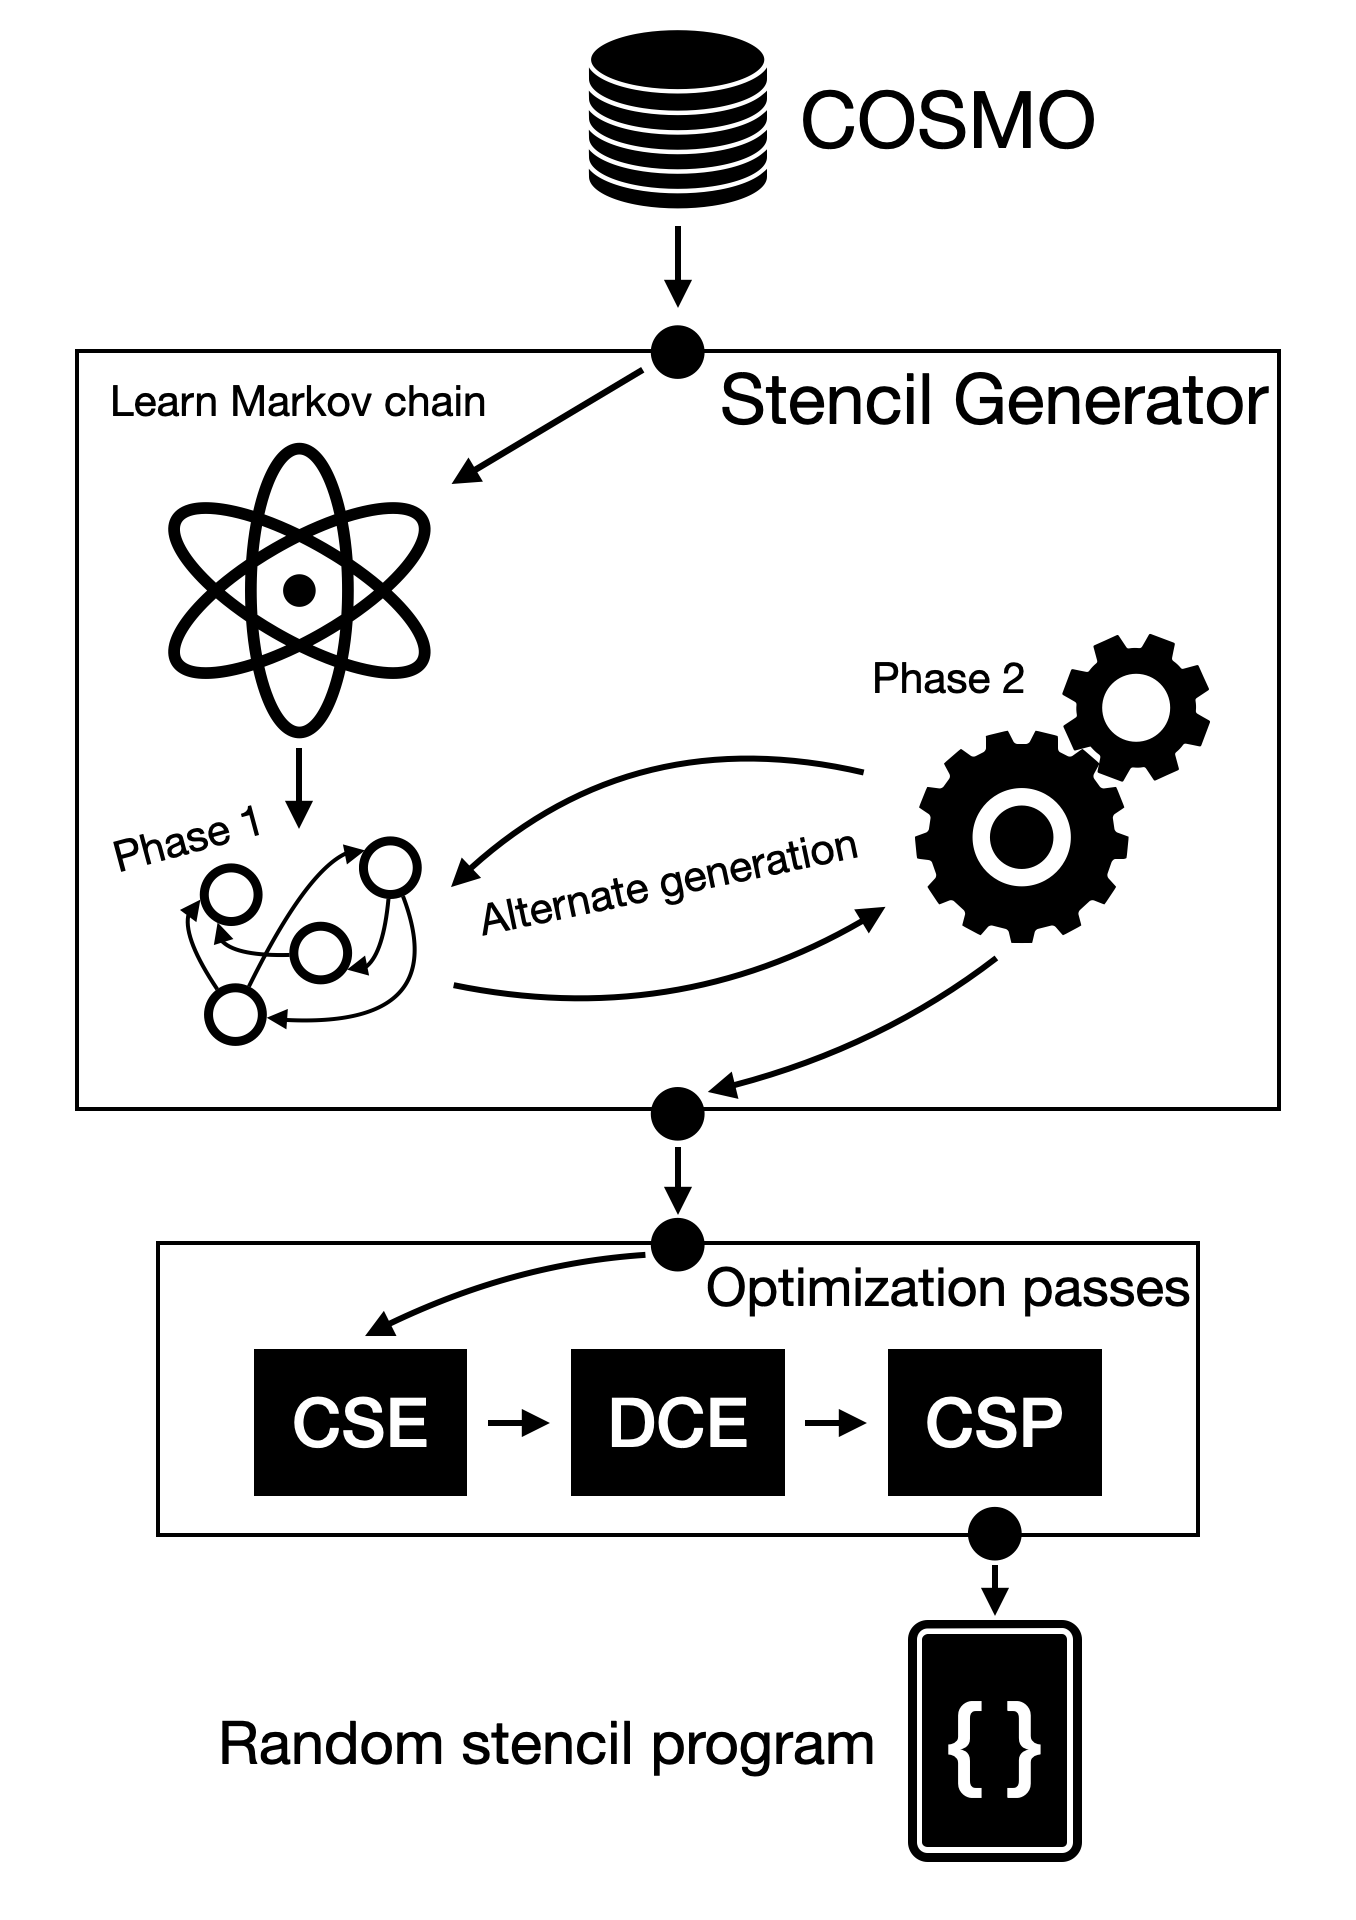
\includegraphics[width=\columnwidth]{images/rspg_diagram.png}
  \caption{ Diagram shows the generation pipeline. It takes COSMO stencils as
  an input, learns a Markov chain from them and alternates Phase 1 and Phase 2
  to generate a random program. Finally, optimization passes are run on the 
  generated program to make it look more like human-written. }
  \label{fig:rspg_diagram}
\end{figure}

On the other hand, it has some design limitations which mainly affect the
quality of the generated programs but sometimes even correctness. Some chains
produced by iterating Markov chain are not valid series of operations. The
reason behind it lies in the fundamentals of the Markov chain, where the
probability of each event depends only on the current state. However, in
Stencil programs, some operations depend on more than a previous one or are
entirely independent of it. Therefore there can exist incorrect chains that
cannot be converted by the second phase to a valid program. The simplest
incorrect chain (including operations only inside \texttt{do\_method} body)
would be \texttt{field\_access} $\rightarrow$ \texttt{std.subf}. The chain
is invalid as subtraction requires at least one value, but
\texttt{field\_access} produces only a pointer. Even though the probability
of generating such a chain is very low (0.00374), it is still very likely to
occur when generating huge datasets. Our initial solution to incorrect
program chains was to ignore infeasible operations in the chain. It was
working well until we started to adjust statistics of generated programs to
the ones from COSMO. With this setting, it became very challenging to predict
the length of the generated program as many operations were flagged infeasible,
and thus not considered. Other issues were occurrences of operation pairs that
never occurred in COSMO stencils. These occurrences caused some statistics of
random programs to be different from the COSMO ones. Therefore we decided to
change the way both phases cooperate. Rather than first generating the entire
chain and then passing it to the second phase, which ignores infeasible
operations, we decided for the "on the fly" chain generation. This approach
enables us to use context produced by the second phase in the first one. Based
on the context, we can temporarily remove outgoing edges that would lead from
the current state to an infeasible state. In the new setting, it is not
possible to reproduce the example from above, as this time, we would
temporarily remove all outgoing edges from \texttt{field\_access} that
require at least one value.

The second point where program chains generated with the Markov chain need
some enhancement is their quality. Our criteria for quality is to minimize
the amount of generated dead or easily optimizable code. Mainly, we try to
prevent the need for basic optimization passes like constant propagation,
common subexpression, or dead code elimination. A great example of this
problem would be a ternary operator. Since MLIR is in a static single
assignment form (SSA) and we cannot inline constant values inside expressions,
we need to have defined at least two values in front of it. The first value
needs to have a boolean type, and it is for the condition. The second one is
the return value for both cases. Ideally, we want to have a distinct value
for each branch. Therefore 3 in total. In the Markov chain, a ternary
operator follows a comparison operator with a very high probability, and
thus it is very likely that it will succeed a comparison operator in one
of the generated programs. Now let's assume that before this pair of
operations, there is available only one value X. The resulting program then
has to look like this:

\begin{lstlisting}
%0 = cmpf %X, %X : f64
%1 = select %0, %X, %X
\end{lstlisting}

The comparison operation has to take the value X for both operands. It produces
a boolean value, which will consequently be used together with X by the ternary
operator. This sequence is a valid part of the program but not of high quality
as it will be optimized away. To circumvent cases like this one, we had to
incorporate further chain constraints. However, it is not simple to detect all
code snippets that get optimized away. Therefore, we came up with the following
detection strategy. First, we generated a big dataset of short programs.
Second, we lowered the programs to CUDA files and obtained their register usage
with the help of \texttt{nvcc} with \texttt{ptxas} flag. Finally, we detected
candidates for the optimization by investigating programs using only 2
registers, which means that they became empty after the optimization. The
reason why we generated short programs, was to maximize the probability of a
complete program erasure and thus detection of the code snippets we should
prevent in the generation. Longer programs have a higher probability of not
being completely erased. With this method, we detected that the most common
erasure reason was dead code, followed by a common subexpression elimination
(CSE). We will explain how we partially prevented the generation of this code
in the following subchapter, as it turned out that the Markov chain has very
little influence on it.

We started with the Markov chain as a baseline model. Very soon, we found out
that it has some limitations that more advanced models, like higher-order
Markov chains, might not have, but with a small fix, we were able to solve
the correctness issue as described above. The code quality problem turned out
to be mostly caused by the second phase, and therefore we decided to keep
building on top of it.

\subsection{Generating the Operation Chain}
As already mentioned, we have available around 30 stencils used in the COSMO
atmospheric model. Our goal is to reproduce them in a defined quantity. We use
them to learn the Markov chain as follows: First, we convert each of the input
programs to a chain by iterating each program's IR preorder and appending each
operation type to a list. Second, we create a graph with a node for every
operation type and iterate over the program chains. For each pair of operation
types $(A, B)$, where $B$ follows $A$ in the chain, we increment the weight of
the corresponding edge in the graph. In the last step, we compute outgoing
probabilities by dividing the weight of each edge by the sum of weights of all
outgoing edges. Generated Markov chain from COSMO stencils can be seen in
figure \ref{fig:markov_cosmo}.

\begin{figure}
  \caption{A Markov chain generated from COSMO stencils. The nodes of the graph
  are operation types. The edges are annotated with probabilities.}
  \centering
  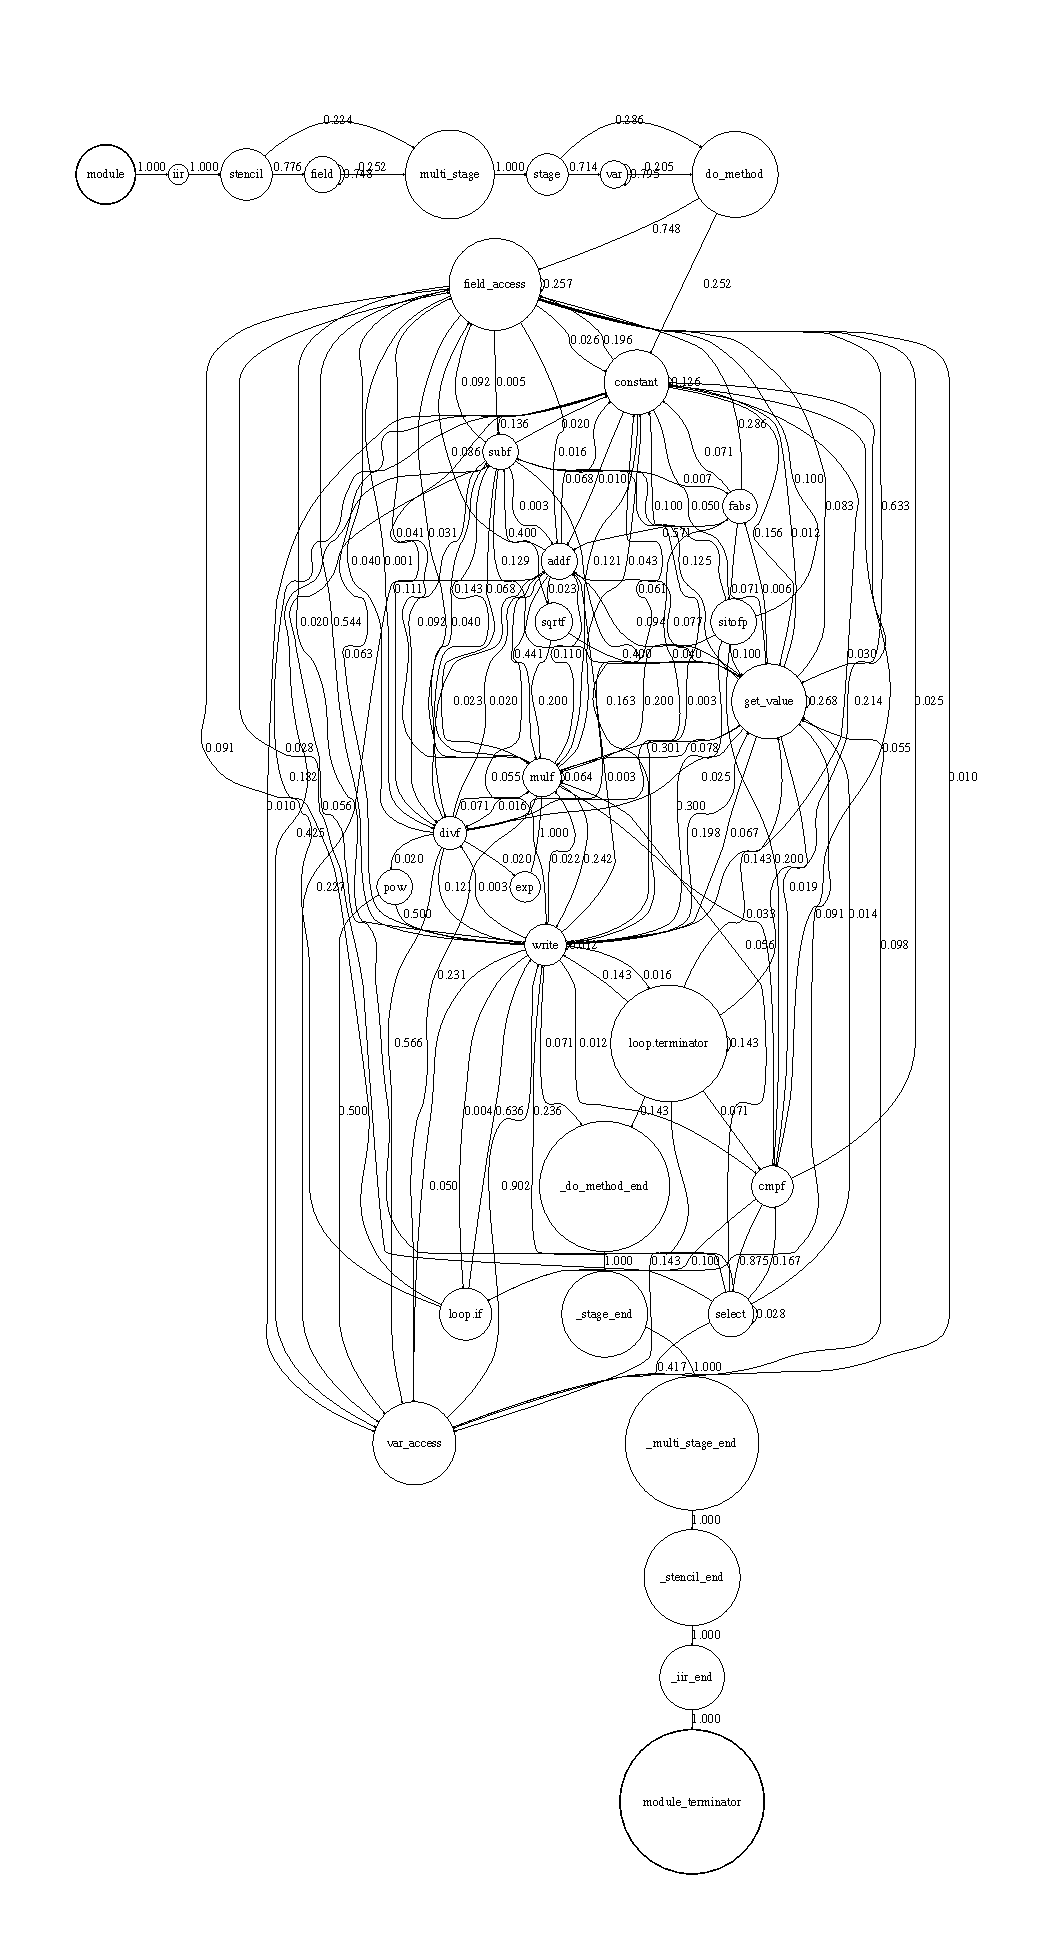
\includegraphics[width=0.9\columnwidth]{images/markov_chain.pdf}
  \label{fig:markov_cosmo}
\end{figure}

We can see that the Markov chain has one starting state, which has no incoming
edges as well as a dead-end stage, which has no outgoing edges. Starting state
is the operation of type \texttt{module} as it is the parent operation for any
MLIR program. Since the module is an operation with a body, it needs to have a
matching terminator op. Its name is \texttt{module\_terminator}, and it is the
"dead-end" state in our Markov chain. It indicates the end of the only
top-level operations body because no other operation is allowed to reside on
the same level as the module. The generation algorithm of random program chains
is as follows:\\

\begin{algorithm}
\begin{algorithmic}[1]
\Function{createRandomProgramChain}{programs, min, max}
  \State $context \gets createContext()$
  \State $chain \gets createMarkovChain(programs)$
  \State $curr\_op \gets "module"$
  \State $end \gets "\_do\_method\_end"$
  \State $curr\_length \gets 0$
  \While {$curr\_op \neq "module\_terminator"$}
    \State $view \gets (s) => isValid(s, context) \land
    i \geq min \land s\neq end$
    \State $curr\_op \gets chain.getNextOp(curr\_op, view)$
    \If {$i = max$}
        \State $curr\_op \gets end$
    \EndIf
    \State $secondPhase(curr\_op, context)$
    \State $curr\_length \gets curr\_length + 1$
  \EndWhile
\EndFunction
\end{algorithmic}
\caption{Pseudocode for sampling a chain from the Markov chain.\label{alg:chain_generation}}
\end{algorithm}

"On the fly" generation starts in the initial state of the Markov chain. First,
we temporarily remove all outgoing edges that lead to invalid states based on
the context, which is updated by the second phase after processing the current
state. Second, we update the probabilities of the outgoing edges such that they
still form a probability distribution and sample a new state from it. We add
back all temporarily removed edges and recompute original probability
distribution. Finally, we set the sampled state to the current state, run
the second phase on top of it, and repeat the same procedure with the updated
context again. A Markov process can generate infinitely long program chains
but very short ones as well. Therefore, we had to implement other measures
that keep program length in the interval defined by us.

To prevent the generation of very short programs, we always temporarily remove
\texttt{\_do\_method\_end} from the outgoing edges if the current chain length
is shorter than the minimum required length. This removal prevents the Markov
process from entering the stage from which exists only one way, and it leads
to the dead-end stage. To avoid infinite chains, we set the next stage to
\texttt{\_do\_method\_end} if the current chain length exceeds the maximum
allowed length. This rule allows us to control the upper bound of the program
chain, and thus we can adjust the length of generated programs to our needs.

\subsection{Operation Chain Conversion}
The second step in the Stencil program generation is to convert the operation
chain generated by the first phase to a program in the Stencil MLIR dialect.
As already mentioned in the previous chapter, we decided to change the
generation pipeline. Instead of separating both phases, we decided to let them
interleave on every operation. Therefore the second phase needs to be modular
so it can handle the conversion of a single operation type to a concrete
instantiation of it in the  Stencil dialect. Furthermore, it needs to attach
the instantiation to the program IR as well as to update the current context
of the generation. Therefore we have to make this phase stateful as we need a
state for inter-stage information sharing.

As can be seen in algorithm \ref{alg:chain_generation} on line 2, we first
create a context. Context is a data structure that is being used by the
generator for sharing generated values and pointers in between operations.
In the second phase, we receive a chain of operation types together with their
program order produced by the first phase. To generate a valid MLIR program,
we need to create new instances from the operation types and attach them to
the program IR. If we want to create a new operation instance, we need to
ensure that we give it valid as well as meaningful arguments. Furthermore,
we need to share the result of every operation with the following operations
so that they can use it as an argument. Context provides both of these
functionalities, and its structure is as follows:

\begin{itemize}
  \item \textbf{fields} : \texttt{UniformDistribution} of the input 
    \texttt{Fields}
  \item \textbf{vars} : \texttt{UniformDistribution} of the variables 
    defined before \texttt{DoMethod}
  \item \textbf{read\_pointers} : \texttt{ExponentialDistribution} of the
    pointers that can be read
  \item \textbf{write\_pointers} : \texttt{ExponentialDistribution} of the
    pointer that can be written
  \item \textbf{values} : \texttt{ExponentialDistribution} of the
  \texttt{double} values that can be used in the computation or
  can be written to a pointer
  \item \textbf{bool\_values} : \texttt{ExponentialDistribution} of the
  \texttt{boolean} values that can be used in \texttt{If} conditions 
  or \texttt{Select} operations
\end{itemize}

We are using two types of distributions for two different scenarios. Fields
and variables are always bulk inserted into the context as they are defined
only at one place each. All fields come as arguments of the \texttt{Stencil}
operation. Similarly, all variables definitions are in a row before the
\texttt{DoMethod}. Therefore, we give every field as well as every variable
equal chance to be sampled and thus be used by some operation. 

On the other hand, we give the exponential distribution to all other context
fields because they are no longer defined at the same place, but their
definitions are spread throughout the entire body of the \texttt{DoMethod}.
If we had used the uniform distribution, it would have made it unfair for the
recently defined values as the older ones already had more chances to be
sampled. Furthermore, in a human-written code, most recently defined values
have much higher chances of being used in the current expression than the older
ones. Therefore we decided to model this distribution as the exponential one.
In other words, the most recently defined value has the same chance of being
sampled as all older values combined. Another advantage of this distribution
is the contribution to the reduction of the need for dead code elimination as
it maximizes the usage of the distinct values. If we had used the uniform
distribution, the values defined at the beginning of the program would have
had a much higher chance of being used in some expression. Moreover, they would
be sampled multiple times while values defined at the end of the program would
not be sampled at all, and thus their definitions would become dead code.

We split the fields in the context into two groups: read and write ones.
Initially, we had only one group for all pointers, but later we observed
that this approach is responsible for the generation of redundant operations
that are erased by the CSE optimization pass.

In our setting, we always ensure the generation of unique field accesses.
Therefore pointer aliasing is not possible as all pointers always point to
distinct parts of the memory. This fact allows us to optimize pointer reads
and writes more drastically with two optimizations. The first one removes the
second of the two consecutive reads and replaces all its usages with the value
from the first read as it would read the same value. The second optimization
removes the first of the two consecutive writes to the same pointer as the
first write gets always rewritten by the second write.

These two optimizations are the reason why we decided to split all pointers
into the read and write group and introduced the following rules for the
insertion and removal. Every time a field is accessed, and thus a new pointer
is produced, we insert it to both groups as field entry can be either read or
written. On the other hand, when a variable is accessed, we insert the produced
pointer only into the writing group as read of an uninitialized variable causes
undefined behavior. Furthermore, two more operations consume pointers. The
write operation writes to a pointer, and thus it first samples from the write
pointers, then it removes the sampled element, and finally, it inserts the
element to read pointers, as we don't want to have two writes to the same
pointer in a row. Similarly, read operation samples from the read pointers,
removes the sampled operation, and inserts it into the write pointers.

Another relevant line in algorithm \ref{alg:chain_generation} is the definition
of a view. View is a lambda function applied to every outgoing edge from the
current state. If the function returns false for some edge, we do not consider
it for sampling. We use this view for temporal edge removal by applying it in
each stage on top of the Markov chain.

The view function consists of three conditions joined by a conjunction. The
second part: $i \geq min \land s \neq "\_do\_method\_end"$ controls the minimal
program length by prohibiting the Markov chain to sample the next method state
because it leads to an end state. The first part is more critical as it ensures
both correctness and quality by filtering out states that either cannot be
processed with the current context or would result in dead code. The algorithm
\ref{alg:isValid} shows the rules that filter invalid stages based on the
current context.

In the following list, we are going to explain the logic behind every rule and
show how it improves both quality and correctness. We numbered the rules as
they appear in the code and state line number for each rule as well.

\begin{algorithm}
\begin{algorithmic}[1]
  \Function{isValid}{op, context}
    \If {$op = "stencil.field\_access" \land context.fields.empty()$}
    \State \Return $false$
    \ElsIf {$op = "stencil.var\_access" \land context.vars.empty()$}
      \State \Return $false$
    \ElsIf {$op = "stencil.get\_value" \land context.read\_pointers.empty()$}
      \State \Return $false$
    \ElsIf {$op = "stencil.write" \land$\\
        $(context.write\_pointers.empty() \lor context.values.empty())$}
      \State \Return $false$
    \ElsIf {$op = "std.select" \land$\\
    $(context.values.size() < 2 \lor context.bool\_values.empty())$}
      \State \Return $false$
    \ElsIf {$op = "loop.if" \land (context.bool\_values.empty())$}
      \State \Return $false$
    \ElsIf {$op$ \texttt{in} $unOps \land context.values.empty()$}
      \State \Return $false$
    \ElsIf {$op$ \texttt{in} $binOps \land context.values.size() < 2$}
      \State \Return $false$
    \EndIf
  \EndFunction
\end{algorithmic}
\caption{Rules of the \texttt{isValid} \textit{view} function.\label{alg:isValid}}
\end{algorithm}

\begin{itemize}
  \item \textbf{Rule 1} (line 2) \texttt{FieldAccess} 
  operation requires one field as an argument. Therefore we need to have at least
  one in the context. This rule ensures correctness as it prohibits to enter
  the invalid state.
  \item \textbf{Rule 2} (line 4) \texttt{VarAccess} 
  operation requires a variable as an argument. Therefore we cannot enter
  this state without having at least one in the context.
  \item \textbf{Rule 3} (line 6) \texttt{GetValue}
  operation dereferences a read pointer, and thus it needs to have some
  available.
  \item \textbf{Rule 4} (line 8) \texttt{Write}
  operation requires a pointer and a value that is written to it.
  Therefore we need to have both them available.
  \item \textbf{Rule 5} (line 11) \texttt{Select},
  in other words, ternary operator, requires one boolean value for the
  condition and 2 values for both branches.
  \item \textbf{Rule 6} (line 14) \texttt{If}
  operation requires only one boolean value for the condition.
  \item \textbf{Rule 7} (line 16) \texttt{Unary}
  operation requires one value as an argument.
  \item \textbf{Rule 8} (line 18) \texttt{Binary}
  operation requires at least one value. However, the only meaningful binary
  operation with both operators the same is multiplication \texttt{x * x} and
  addition \texttt{x + x}. Since multiplication can be replaced with
  \texttt{pow(x, 2)}, and addition with multiplication \texttt{2 * x}, we
  decided to increase the quota to 2 to prevent the generation of easily
  optimizable operations.
\end{itemize}

\subsubsection{Accumulators}
To successfully create a Stencil operation in MLIR, we need to know three
things: type of the operation, location in the IR, and its arguments. We
can further divide arguments into two groups. The first one consists of the
ones that are results of the other operations, and thus we call them dependent
arguments. The second group contains arguments that are independent of any
previous operations as they depend only on their type. Therefore we will call
them independent arguments.

So far, we have available all elements needed for the construction of
operation except for the independent arguments. Type of the operation
and its location can be inferred from the operation chain, while dependent
arguments can be sampled from the context. Furthermore, when creating an
operation, we can always assume that it is constructible. The last missing
piece in our puzzle is to create independent arguments.

As already mentioned, a large part of the operation types has independent
arguments. Since they are independent, we can isolate their learning and
sampling processes per operation type. For that purpose, we created an
accumulator for each operation containing independent arguments. In the
following list, we are going to explain each accumulator, which arguments
it accumulates, and how they are later sampled.

\begin{itemize}
  \item \textbf{Field Access Accumulator} \texttt{FieldAccess} operation
  takes as an argument a field and an offset. A field is sampled from the
  context since it is a dependent argument. An offset needs to be generated.
  This accumulator extracts all field accesses from all learning programs
  and forms a distribution where the probability of sampling an offset
  increases with the number of its occurrences in the learning programs.
  Therefore, the generated offset is never unique but rather one of the
  offsets occurring in the learning programs.

  \item \textbf{Constant Accumulator} \texttt{Constant} operation is one
  of the operations that does not contain dependent arguments, and therefore
  can be placed in the program anywhere from the beginning till its first
  usage. The only parameter it takes is the actual number. In this case,
  we first started with collecting maximal and minimal constant occurring
  in the learning programs. However, it turned out to not be working well
  as constants in the COSMO model have their meaning, while constants in our
  stencils were just random numbers generated in the large range. Therefore
  we adopted the same approach as in the case of \texttt{FieldAccess}
  - we stopped to introduce unseen constants. Instead, we sampled from values
  seen in the learning programs with probabilities adjusted for counts.

  \item \textbf{MultiStage Accumulator} \texttt{MultiStage} operation does
  not contain any dependent arguments, only one independent - an order in
  which it evaluates the child stages. Since it can take only a very
  restricted list of values, we compute cardinality for each of them and
  adjust probabilities accordingly.

  \item \textbf{DoMethod Accumulator} \texttt{DoMethod} operation has four
  independent arguments, which are lower bound, lower offset, upper bound,
  and upper offset. Our initial approach was to collect ranges for each of
  these four values. It worked well, but we decided to not generate novel
  ranges since they were not useful for us. Furthermore, the experiments we
  do in the next chapter required a low variance across these values.
  Therefore we decided to sample from the accumulated values with
  probabilities computed according to cardinalities.

  \item \textbf{Access Pattern Accumulator (experimental)} We implemented 
  one more accumulator, which is not meant for a single operation but rather
  for a group of operations that we decided to call the access pattern. It
  consists of one or more \texttt{FieldAccess}, \texttt{VarAccess}, and
  \texttt{GetValue} operations. We observed in the COSMO stencils that fields
  tend to be accessed in groups together with variables. Furthermore, a couple
  of \texttt{GetValue} operations follow to obtain values from the pointers.
  Therefore we decided to model this behavior with access patterns. First,
  we extract all access patterns from the learning programs. We do extraction
  by searching for subsequences containing only one of the three types
  mentioned above. From the subsequences, we extract offsets, fields, variable
  IDs, and store them to a list. Later, we create a new access pattern by first
  filtering the list of accumulated patterns based on the number of fields and
  variables it requires. We need to filter out patterns that require more
  fields or variables than we have available in the context. In the second
  step, we sample from this filtered uniform distribution by sampling the
  required number of fields and variables from the context and creating needed
  operations with the help of the other accumulators.

  We tried to generate programs with this new setting by replacing the direct
  generation of field and variable accesses with access patterns. However,
  resulting programs did not significantly differ from the ones generated
  without access patterns. Therefore we decided to keep the old version as
  the default one. We decided to keep the code for the access patterns for
  further experimenting.

\end{itemize}

\subsubsection{Building the IR}

Now we have all components ready for joining them together. As already
mentioned, we are alternating both phases for the optimal results. The reason
for the alternation is the context that is being updated by the second phase
and read by both phases. As can be seen in algorithm \ref{alg:chain_generation}
line 13, we designed the second phase to handle conversion from operation type
and context to a new instance. So far, we explained how we create or sample
arguments, but we did not explain how we attach the new operation to the IR.

The second phase function is a mapping between operation type and a function
that handles its construction. All construction functions have a unified
signature. They take a context as the only argument. Furthermore, they
internally share an instance of the \texttt{Builder} class, which is an MLIR
construct for creating new operations. The \texttt{Builder} not only creates
new instances but also attaches them to the IR as it keeps track of the
current insertion point. Therefore, it simplifies the entire process as we
don't need to modify the IR ourselves.

For every new instance, except for the \texttt{Module}, we assume that the
\texttt{Builder} has the insertion point set correctly. The \texttt{Module}
is a very specific operation. Since it has no parent, there is no insertion
point possible during its construction. Therefore we have to create the module
without a builder and set the insertion point to its body once we create it.
For all operation types that have a body, we need to set the insertion point
to the beginning of the body after we create their instance. The
\texttt{Builder} will create all the following operations inside the operations
body. For all terminators, we need to update the insertion point again as they
end the parent operations body. Therefore we move it one level up, right behind
the parent operation.

\subsubsection{DCE, CSE and CSP Passes}
Even though we tried our best, we were not able to completely prevent the
generation of the code that can be optimized or erased. Furthermore, we
detected that COSMO stencils have some space for optimization as well.
Therefore we decided to use the optimization passes to get rid of the
unnecessary code. We wrote some passes ourselves as well as we used the
Common Subexpression Elimination (CSE) pass from the MLIR toolkit. We run
these passes on the generated programs at the very end of our pipeline.
In this subchapter, we are going to describe each of the passes.

\paragraph{Dead-code elimination (DCE)} pass is responsible for recursive removal of 
the dead code. An operation in Stencil dialect is considered dead if there
are no usages of its result or if all operations using its result are
considered dead. Therefore, in dead code removal, we have to start the
analysis from the back of the basic block. We don't need a recursive lookup
when iterating a block backward because we already checked all its usages.

Another optimization, DCE pass performs, is flattening of \texttt{If}
operation. If we can evaluate the value inside the condition during
compilation time, we flatten the corresponding body of the \texttt{If}
operation. The second body is erased as it will never be executed.
If both bodies are found empty, we completely erase the \texttt{If} operation.

\begin{lstlisting}[caption={A code sequence before DCE pass}
  ,captionpos=b,label={lst:dce_before}] 
%0 = stencil.field_access %arg0 [0, 0, 0]
      : !stencil<"ptr:f64">
%1 = stencil.field_access %arg1 [0, 0, 0]
      : !stencil<"ptr:f64">
%2 = stencil.get_value %0 : f64
%3 = stencil.get_value %1 : f64
%4 = addf %3, %2 : f64
stencil.write %1, %2 : f64
stencil.write %1, %4 : f64
%5 = stencil.get_value %1 : f64
stencil.write %0, %5 : f64
\end{lstlisting}

The last optimization, this pass does, is a field and a variable propagation.
We know that memory accesses are expensive operations, and thus it is always
beneficial to minimize them. Furthermore, any unnecessary operation confuses
machine learning models more in their predictions as they lack deep program
understanding. In listing \ref{lst:dce_before}, is an example of a program
before the DCE pass. This program performs one unnecessary read and write.
The write at line 8 is redundant as the write at line 9 will rewrite it.
Therefore we can safely remove this operation. The read at line 10 can be
removed as we know the value that will be read. The resulting program sequence
can be seen in listing \ref{lst:dce_after}.

\begin{lstlisting}[caption={A code sequence after DCE pass}
  ,captionpos=b,label={lst:dce_after}] 
  %0 = stencil.field_access %arg0 [0, 0, 0]
        : !stencil<"ptr:f64">
  %1 = stencil.field_access %arg1 [0, 0, 0]
        : !stencil<"ptr:f64">
  %2 = stencil.get_value %0 : f64
  %3 = stencil.get_value %1 : f64
  %4 = addf %3, %2 : f64
  stencil.write %1, %4 : f64
  stencil.write %0, %4 : f64
\end{lstlisting}

We can generalize this example to two optimization rules.
\begin{enumerate}
  \item Every time, we encounter two write operations to the same pointer in
  a row, i.e., they are not interleaved by the read operation, we safely
  remove the first one. 
  \item Every time we encounter a pointer that is first written and
  then read within the same basic block, we remove the read operation and
  replace all its usages with a value that is written to the pointer.
\end{enumerate}

\paragraph{Common subexpression elimination (CSE)} pass is an MLIR pass that
reduces program length by searching for duplicate common subexpressions and
removes all but one. It performs some limited dead code elimination as well.
However, the CSE pass is not able to propagate fields and variables, and thus
DCE and CSE pass form a powerful optimization pipeline. This pass comes as a
part of the MLIR.

\paragraph{Constant propagation (CSP)} pass is a well-known optimization that
we implemented because we observed many binary expressions that had constants
as both operands.\\

To sum the entire generation process up, we first create the Markov chain,
which is a directed graph with nodes being states and edges transitions
between them. In our case, nodes are operation types. We learn the
probabilities in the Markov chain from the COSMO stencils as we want to
replicate them. However, our approach is general enough to replicate other
datasets. 

Second, we introduced the context as a way of sharing state between stages.
In the first stage, we need the context for filtering invalid stages while
in the second stage, we use it for sharing of values and pointers between
operations. 

Third, we introduced the second phase together with accumulators. The second
phase creates new instances from operation types and context. It does it by
having a mapping between operation type and a handler function. Each handler
function is responsible for creating an instance of a different operation
type by using the context and particular accumulator. Accumulators are
classes that are responsible for the accumulation and sampling of independent
arguments. We divide arguments into two groups. Dependent arguments are values
or pointers that are produced by other operations. We call them dependent
because they depend on the other operations. The second group is independent
arguments. The group consists of arguments that are independent of other
operations. A good example would be a field offset. 

Lastly, we explained how we used the MLIR \texttt{Builder} class for building
program IR. The builder uses an insertion point as the location for new
instances it creates. We change the insertion point when we encounter an
operation with a body or a terminator. The result of this process is a valid
program in MLIR Stencil dialect.

\subsection{Evaluation}
In the previous subchapters, we introduced a method of replicating some dataset
into a much larger one by learning its structure. Furthermore, we described the
problems we encountered along the way, the enhancements we did to increase the
similarity of generated programs to the learning ones. In this subchapter, we
are going to evaluate the dataset of stencil programs generated by us with the
COSMO one.

We can define the objectives of our entire approach in two words: correctness
and quality. We further split correctness into two types. The first one is the
correctness of the generator. Here we had to ensure that we never generate a
state which cannot be constructed. While it is hard to prove the correctness
mathematically, we generated a sufficiently large amount of random programs
without entering the invalid state. Therefore we gained confidence that the
generator works at least for the COSMO stencils very well. The second type
concerns the correctness of generated programs. The mathematical proof for
this type of correctness is even harder as we would need to prove that every
generated program is a correct program. Furthermore, we found it equally
challenging to come up with a testing infrastructure for random programs
because the correct result is not known to us either. Therefore, we left this
task for future research.

The second objective of our approach is the quality of the generated programs.
We came up with two measures to assess it. The first one is an internal one.
We measure how many lines of code get erased by DCE, CSE, and CSP pass. This
measure indicates how much unnecessary code we generate. As already discussed
in the previous subchapter, we cannot entirely prevent the generation of
dead-code. However, it is still interesting to observe how some measures
influence this number. In the case of the CSE pass, we could have prevented
the duplicate generation of subexpressions. However, we decided to prevent
only the generation of duplicate variable accesses, field accesses, and pointer
dereferences. We did not prevent the generation of the common subexpressions
because we would just duplicate the functionality of the CSE pass. The final
versions of the generated programs have all of these passes applied. Therefore
the final effect would have been the same.

\subsubsection{Evaluation of the Optimization Passes}

As already mentioned, one of the measures for the stencil program generator is
the amount of easily optimizable code it generates. For some program
generators, easily optimizable code is the desired property because their goal
is to test the optimization passes in the compiler. However, we use our random
programs for training machine learning models that are not capable of deep
program understanding. For instance, we cannot train a statistical model on
a program with dead code as the model would treat it as a normal code, and thus
it would introduce an inconsistency between the program features and the ones
to be predicted.

Our first approach in dealing with dead code was to remove it during the code
generation. Later, we decided to move it into a separate optimization pass as
we needed it for optimizing COSMO stencils as well. This move made our
generation pipeline more modular, and we were able to trace the bugs more
efficiently.

On top of figure \ref{fig:cse_dce_csp_comparison}, we can see the optimization
pipeline. First, we generate "raw" programs, which are later polished by our
optimization passes. The pipeline order is very important as the DCE pass
makes some assumptions that are fulfilled only by the CSE pass. Below the
pipeline, are confidence intervals that display a percentage of a program that
is removed from the previous stage. On average, passes remove more than half
of the "raw" program. In most cases, the CSP pass removes zero lines because
constant propagation can rarely be applied. On the other hand, generated
programs contain a high percentage of dead code and common expressions.

\begin{figure}[!htb]
  \centering
  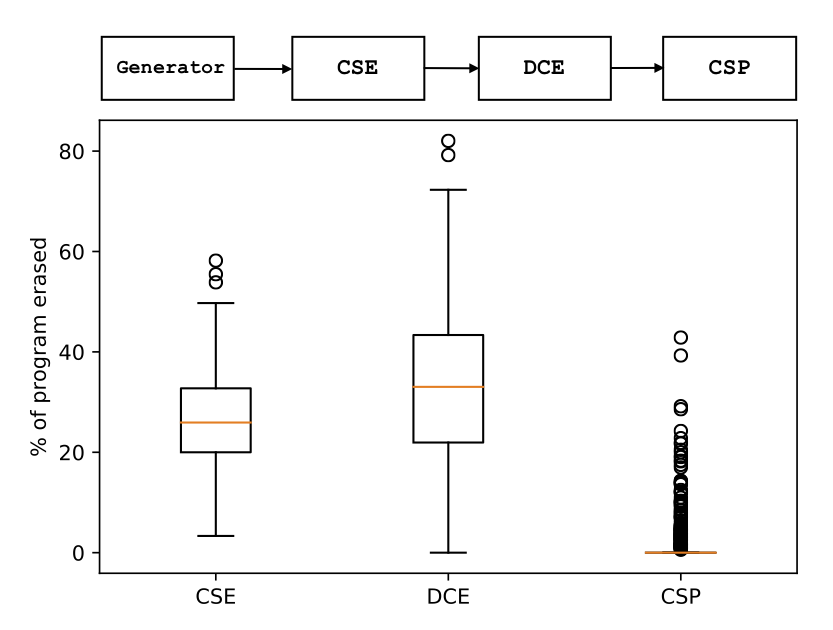
\includegraphics[width=\columnwidth]{images/cse_dce_csp_comparison.png}
  \caption{Optimization pipeline. The plot below shows how many percent
  of a program are being erased by the optimization stage in the pipeline.
  The evaluation dataset consists of 1000 random Stencil programs generated
  by our generator.}
  \label{fig:cse_dce_csp_comparison}
\end{figure}

\subsubsection{Evaluation of the Generated Stencil Programs}

Complete prevention from dead code generation would mean that every result
of every non-void operation needs to be used. To achieve that, we would need
to write all unused results to distinct field pointers at the end of the
program. For that, we would most likely have to create new pointers. This
would result in programs not similar to the COSMO ones as they would all
have many write operations at the end of their \texttt{DoMethod}s. Therefore,
we adopted the opposite approach, where we generate longer operation chains,
which result in larger stencils. Consequently, optimization passes shorten
them, so they end up having, on average, the same length as COSMO stencils.
Figure \ref{fig:gen_vs_dced_top_features} shows a comparison between lengths
of generated and optimized stencils, while figure
\ref{fig:gen_vs_val_top_features} displays a comparison between optimized and
validation (COSMO) stencils. We can see that only around 60\% of the generated
stencils are shorter than 100 lines, while in the case of optimized stencils,
it rises to 90\%. The same applies to the number of unique SSA values where
this number increases from 76\% to 96\% because arithmetic expressions are
the most frequently marked as dead. On the other hand, maximal expression
depth is not affected, which indicates that deeper expressions are less
likely to be eliminated, and they have a higher chance of being written to
a field. Furthermore, average reuse distance increases as dense expressions
which reduce it are removed.

\begin{figure}
  \centering
  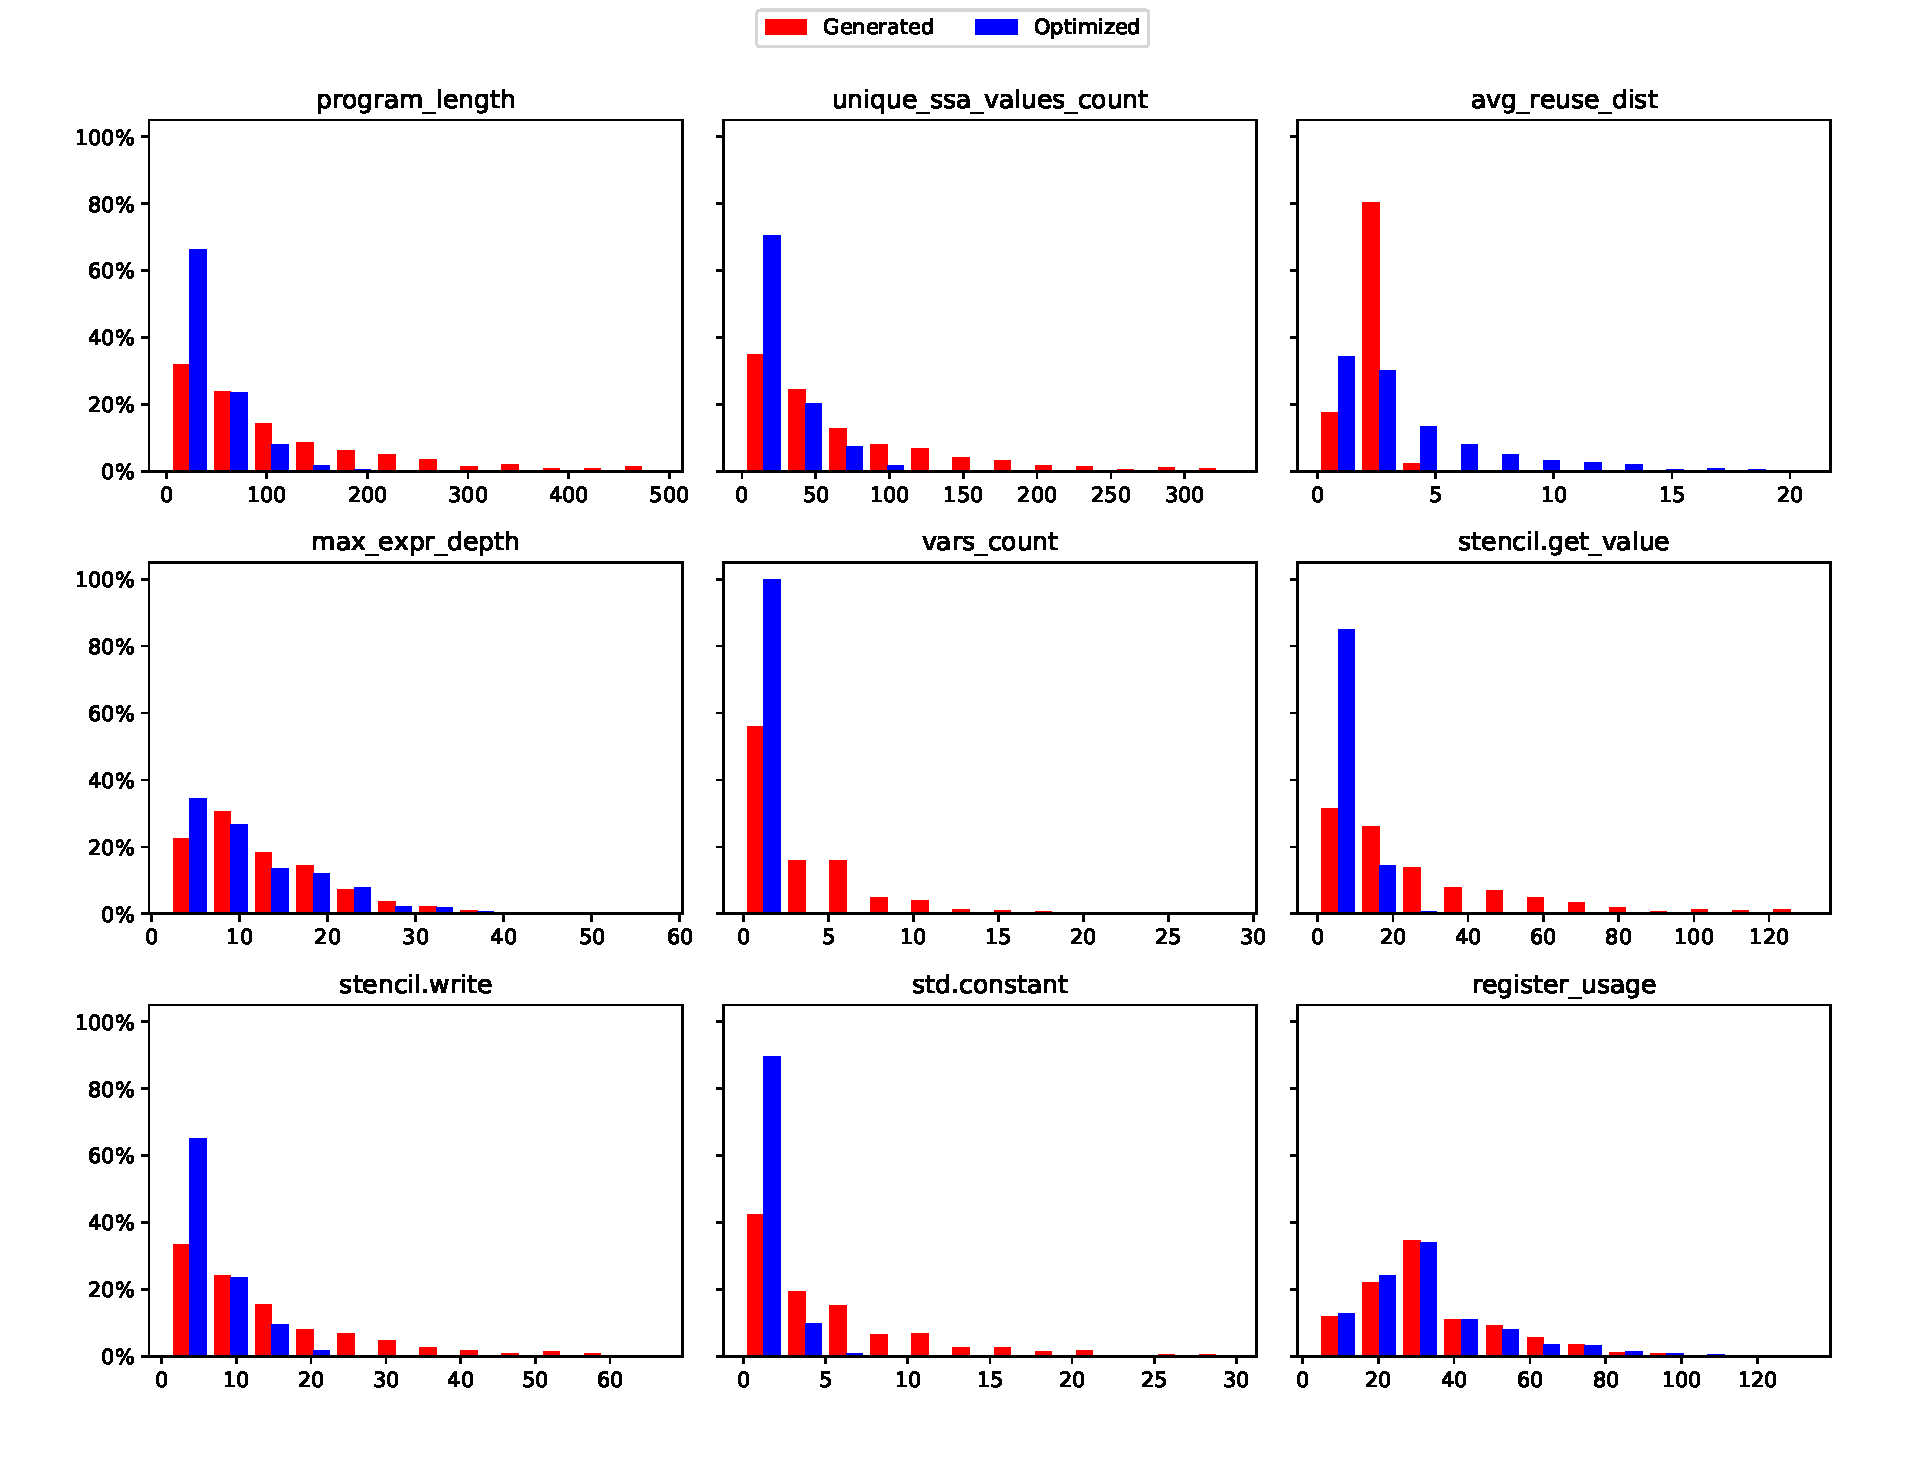
\includegraphics[width=\columnwidth]{images/gen_vs_dced_top_features.pdf}
  \caption{A comparison between random programs before and after optimization
  passes. Each of the plots shows a distribution of one program feature. We
  can observe a shift toward lower values in most plots as optimized stencils
  are much shorter. Register usage changes slightly because optimized
  stencils are semantically equivalent.}
  \label{fig:gen_vs_dced_top_features}
\end{figure}

The plot in the middle shows that optimization passes remove all variables.
As we were writing optimization passes, we realized that in our setting,
there is no need for variables. The only exception is a variable which is
written in both branches of an \texttt{If} operation and subsequently read.
The reasons why we can replace variables inside \texttt{DoMethod} are
summarized in the following points:
\begin{itemize}
  \item Values in variables cannot be shared between \texttt{DoMethod}
  iterations, as they do not have default values, and therefore first
  read in the first iteration is undefined unless it is a write operation,
  in which case value from the previous iteration is always rewritten.
  \item We can propagate variable writes to their subsequent reads,
  remove first of the two writes in a row and remove the last write as
  it will never be read.
  \item The only case when we cannot remove variable is, as already
  mentioned, a variable that is written in both branches of \texttt{If}
  operation because we cannot do the value propagation in this case.
\end{itemize}

CSE and DCE pass cause a massive reduction of \texttt{GetValue} and
\texttt{Write} operations, as shown in the middle right and bottom left plots,
respectively. We attribute \texttt{GetValue} reduction mainly to the
elimination of common field accesses and consequent elimination of
\texttt{GetValue} operations. The second reason is the write to read
propagation mentioned a few times already. It partially causes \texttt{Write}
operation removal as well. The second contributor to \texttt{Write} operation
elimination is the removal of the first of two \texttt{Write} operations
in a row. Lastly, dead code elimination removes some of the \texttt{GetValue}
operations as well, while the \texttt{Write} operation is never dead.

Figure \ref{fig:gen_vs_val_top_features} shows a comparison between the
optimized version of our random stencil programs and validation stencils,
which we obtained from the COSMO model. This comparison was the main objective
for our generator as it shows how close our stencils are to the real ones.
This figure has only six but the most important subplots. We attached the
full comparison of all features for both figures in the appendix. 

\begin{figure}
  \centering
  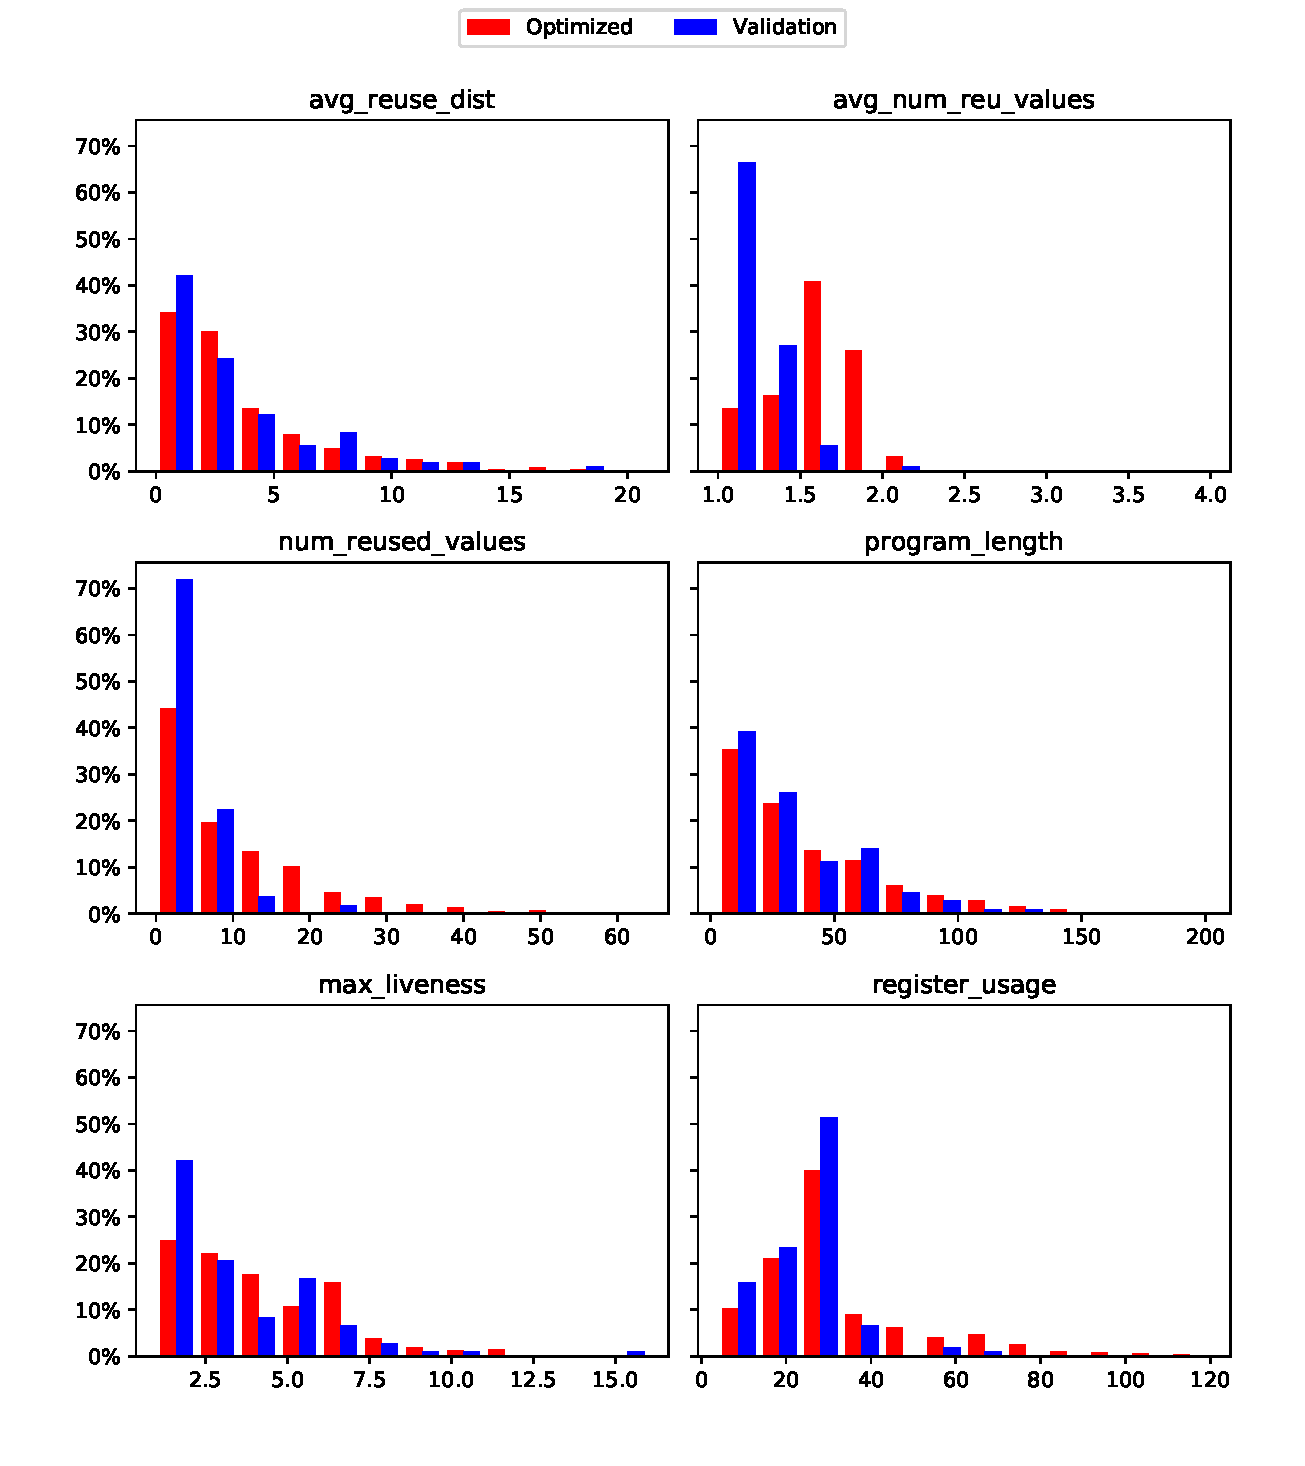
\includegraphics[width=\columnwidth]{images/gen_vs_val_top_features.pdf}
  \caption{A comparison between random stencils generated by us and validation
  stencils from the COSMO model. Each of the plots compares a distribution of
  one program feature. Our stencils match all features of validation ones
  except for the average number of reused values where we reuse one value on
  average slightly more.}
  \label{fig:gen_vs_val_top_features}
\end{figure}

All selected features compared in figure \ref{fig:gen_vs_val_top_features}
are not related to any concrete operation, as this would be easy to replicate.
For instance, generating a dataset where we set the objective to match the
quantity of each operation type would be much easier to generate as the one
where we would compare maximal expression depth. Therefore we decided to
select the "deep" features as our objective because they express the
information about the program's structure. For instance, register usage
cannot be tricked with dead code as the underlying \texttt{nvcc} compiler
would optimize it away and allocate fewer registers.

In the following list, we are going to explain each subplot in the more
details starting from the top left:
\begin{itemize}
  \item \textbf{avg\_reuse\_dist:} Average reuse distance is the number of
  distinct values accesses between two consecutive usages of the same value.
  Therefore, this statistic includes only values that are used more than once.
  As can be seen, we are replicating this feature accurately by not producing
  too long reuse distances. This feature is mainly influenced by the
  distribution we use for value and pointer sampling. The exponential
  distribution is thus modeling the value usage correctly.

  \item \textbf{avg\_num\_reu\_values:} This feature denotes the average number
  of times a value is reused. Here we can see that the validation stencils
  tend to reuse values less. Furthermore, this subplot shows where our
  generator can be improved. Real stencils tend to read the fields in a group,
  compute a new value from them, and write it back to some field. Our stencils
  differ in one point. They share intermediate values between various
  computations, which causes higher value reuse.

  \item \textbf{num\_reused\_values:}  This subplot compares the number of
  values that are used more than once. Again, it shows that our stencils
  reuse values more than COSMO ones, but this time the difference is smaller
  because the quantity is not taken into account.

  \item \textbf{program\_length:} We are capable of replicating program
  length accurately because we can control the upper and lower bound on
  the Markov chain. We aim for the generation of longer sequences, as we
  know that a big portion of the program will be removed by the optimization
  passes. Therefore we set the lower bound to 20 and upper bound to 500, so
  most of the optimized stencils are in the range $\interval[{20, 150}]$.

  \item \textbf{max\_liveness:} Another important feature is the maximum number
  of live variables at any point in the program. Here we tend to have slightly
  more live variables than COSMO stencils due to average higher usage of a
  single value.

  \item \textbf{register\_usage:} This feature is obtained by running
  \texttt{nvcc} with all optimizations, except for loop unrolling, turned on.
  Therefore we cannot fake other features by generating code that can be
  optimized away. Our stencils use approximately the same amount of registers
  as the validation ones. Few high register pressure stencils occur in random
  stencils while not in the validation ones, but we do not treat it as an issue.
\end{itemize}

In this subchapter, we evaluated the optimization passes by comparing features
of stencils before and after their application. Figures
\ref{fig:cse_dce_csp_comparison} and \ref{fig:gen_vs_dced_top_features}
demonstrate that passes were able to remove great parts of the programs while
maintaining roughly the same amount of registers. Moreover, integration tests
were created to assess their correctness.

Furthermore, we evaluated the random stencil generator by comparing random
stencils with COSMO ones. We did it by plotting distributions of the most
important features next to each other. The main objective was to get each
distribution of the generated programs as close to the COSMO one as possible.
The comparison shown in figure \ref{fig:gen_vs_val_top_features} demonstrates
that the random stencil generator can reliably reproduce the COSMO dataset
and thus generate stencils that are suitable for further compiler research.


\section{Experiments \label{sec:Chapter4}}

The motivation behind the random stencil generator is to enlarge the existing
COSMO dataset with new, meaningful stencils that can be used for training
machine learning models predicting either other program features or
optimization strategies. Machine learning models work best when provided with
a noise-free and feature-rich dataset. Furthermore, a dataset has to fully
cover parts of the input space we are interested in. In this chapter, we are
going to explain how we created datasets suitable for machine learning, how
dataset features were selected and collected, and which experiments we tried
with these datasets together with their evaluation and future research
directions.

\subsection{Datasets}
Since machine learning algorithms work with floating-point numbers but not
with a text directly, we had to find a way of representing a stencil program
as a feature vector of fixed size. To do it, we had to identify a set of
features precisely representing a program. The optimal set of features never
represents two different programs with the same feature vector. Furthermore,
each feature vector variable called independent variable should correlate with
at least one predicting variable also called dependant variable.
In other words, if we want to predict some property $y$ of the program
$\lambda$, then at least one feature from the feature vector $X$ of program
$\lambda$ has to have some relationship with property $y$. The most critical
element weakening the relationship is noise. Therefore, our primary goal
before actual feature definition and collection was to clean the generated
stencils off the noise. Initially, we identified dead code as the main source
of the noise, followed by an easily optimizable code. However, this is not a
problem anymore as the optimization passes remove most of it.

\subsubsection{Featurization}
Featurization or feature engineering is the process of using domain knowledge
for feature definition and later extraction. In our case, this was the most
crucial step in the entire experiment as choosing the right features makes
machine learning algorithms work. After some trial and error, the resulting
set of the features looks like this:

\begin{description}
  \item \textbf{loop\_order} An order in which a loop is executed. Can take 3
  values: \textit{forward}, \textit{backward} and \textit{parallel} which we
  map to 1, 2 and 3 respectively.
  \item \textbf{loop\_size} The number of iterations computed as the difference
  between the upper and lower bound. Offsets are not considered.
  \item \textbf{avg\_reuse\_dist} An average reuse distance of all values that
  have more than one usage.
  \item \textbf{avg\_num\_reu\_values} An average number of times a value is
  reused. Here are included all values.
  \item \textbf{num\_reused\_values} Number of values that are reused i.e. used
  more than once.
  \item \textbf{fields\_count} Number of total fields. This is the sum of the
  locally defined fields and fields passed as parameters.
  \item \textbf{unique\_ssa\_values\_count} Sum of all values used in a stencil.
  \item \textbf{max\_expr\_depth} Maximal expression depth. Starts in the read
  of some field or constant and ends in a write of the computed value.
  \item \textbf{bin\_ops\_count} Number of arithmetic operations that have two
  operands.
  \item \textbf{un\_ops\_count} Number of arithmetic operations that have one
  operand.
  \item \textbf{unique\_offsets} Number of unique offsets across all field
  accesses. We do not take the accessed field into consideration, only its 
  offset.
  \item \textbf{program\_length} Length of the body of the \texttt{DoMethod}.
  We do not consider other operations as they are boilerplate code, which is
  not directly translated into CUDA C.
  \item \textbf{max\_liveness} The maximal amount of variables that are live
  at any point in a stencil computed with standard live variable analysis.
  \item \textbf{stencil.field\_access} The number of field accesses. Since
  it is computed on the optimized stencils, it is the number of unique field
  accesses as well.
  \item \textbf{stencil.get\_value} Number of pointer dereferencings.
  \item \textbf{stencil.write} Number of writes to a pointer.
  \item \textbf{std.addf} Number of additions.
  \item \textbf{std.cmpf} Number of comparisons.
  \item \textbf{std.divf} Number of divisions.
  \item \textbf{std.mulf} Number of multiplications.
  \item \textbf{std.subf} Number of substractions.
  \item \textbf{std.select} Number of ternary operators.
  \item \textbf{stencil.sqrtf} Number of square roots.
  \item \textbf{stencil.pow} Number of "raise to power" operations.
  \item \textbf{stencil.fabs} Number of absolute value operations.
  \item \textbf{stencil.exp} Number of "compute exponential function"
  operators. 
  \item \textbf{std.constant} Number of floating-point constants.
  \item \textbf{register\_usage} Number of registers used by a program.
\end{description}


\subsubsection{Data Collection}

Features are extracted from programs in two ways. The first one is by using
custom feature extraction MLIR pass that extracts features from programs
written in the Stencil dialect. The pass iterates Stencil IR, collects
statistics about operation types, reuse distances, etc. and outputs a feature
vector of direct stencil features.

After running the direct feature extraction pass, we have to collect the
remaining feature that cannot be extracted from the source code directly. It
is register usage. In order to extract it, we have to use the following passes
(chained in the listed order) to lower a stencil program to CUDA C:
\begin{enumerate}
  \item Passes from \texttt{mlir-opt}:
  \begin{itemize}
    \item \texttt{--convert-stencil-to-affine} (Written by J.M. Gorius) 
    Lowers stencil dialect to the affine one. 
    \item \texttt{--lower-affine} (Written by MLIR authors) Lowers affine
    constructs to the standard Dialect.
    \item \texttt{--cse} (Written by MLIR authors.) Well known Common
    Sub-expression Elimination.
    \item \texttt{--convert-loops-to-gpu} (Written by MLIR authors) Creates
    kernel and launch function out of two outer loops while keeping the inner
    most inside the kernel function.
    \item \texttt{--gpu-kernel-outlining} (Written by MLIR authors) Outlines
    kernel out of launch function into a separate function.
    \item \texttt{--cse}
  \end{itemize}
  \item Passes from \texttt{mlir-translate}:
  \begin{itemize}
    \item \texttt{--mlir-to-cudac} (Written by us) Converts the mix of GPU
    and standard dialect into \texttt{CUDA C} file. 
  \end{itemize}
\end{enumerate}

Once a stencil program is lowered to \texttt{CUDA C}, we run \texttt{nvcc}
with \texttt{ptxas} flag to get the number of allocated registers, which is
appended to the list of features obtained directly. The feature extraction
process is visualized in figure \ref{fig:feat_coll_diagram}. 

A dataset is generated by running the process described above on top of all
generated programs, accumulating features of all programs into a 2-dimensional
array, and storing it into a CSV file. In the end, we defined 4 types of
datasets we are interested in:

\begin{itemize}
  \item Random stencil programs
  \item Optimized random stencil programs
  \item Validation stencil programs
  \item Optimized validation stencil programs
\end{itemize}

\noindent By \textit{optimized}, we mean a dataset cleaned by
optimization passes. The \textit{validation stencils} are stencils taken
from the COSMO model, which we later use as validation data.

\begin{figure}
  \centering
  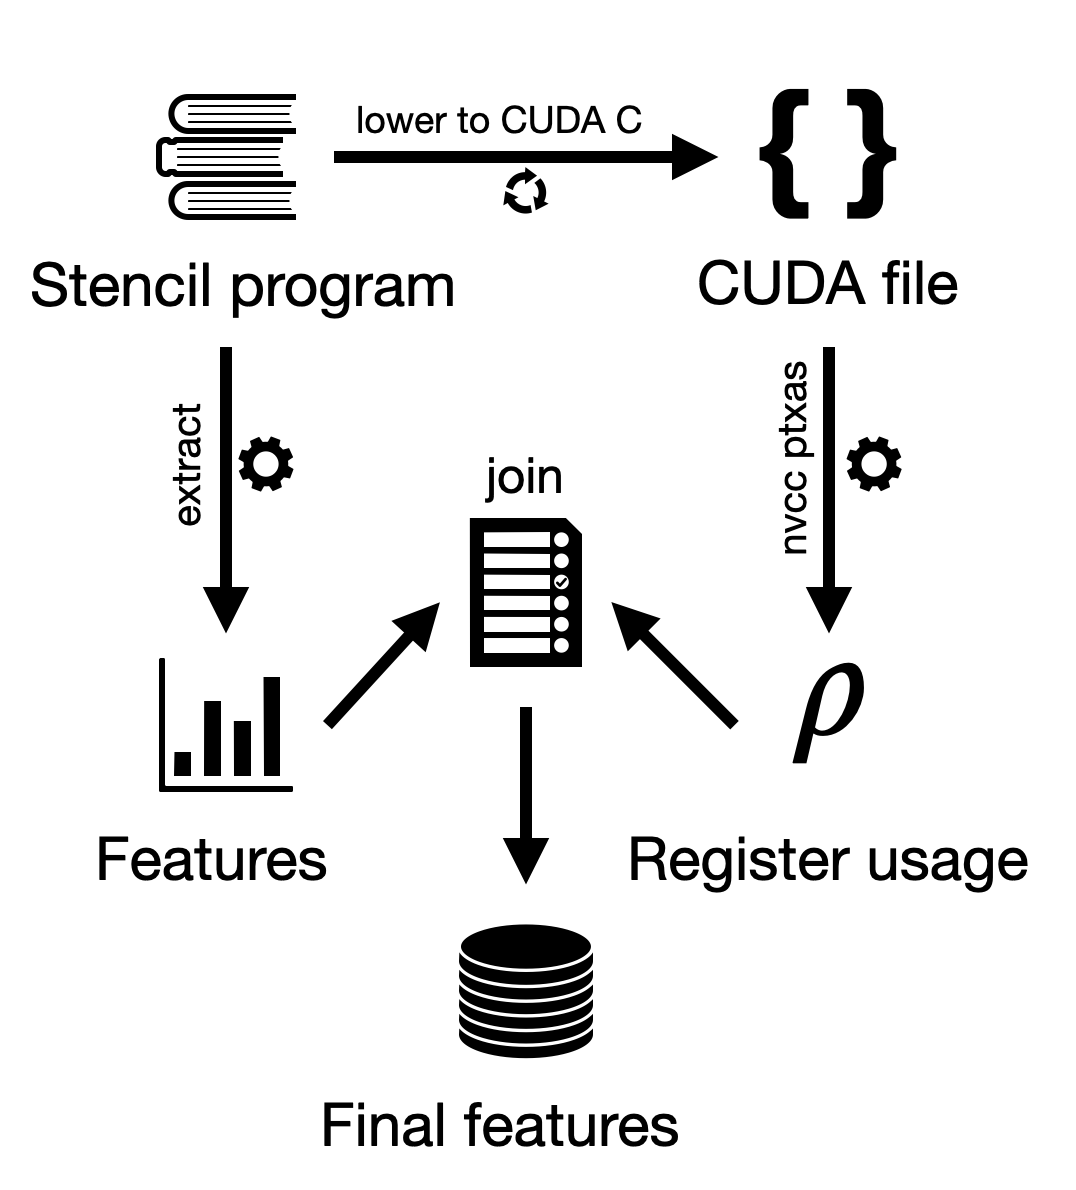
\includegraphics[width=\columnwidth]{images/feat_coll_diagram.png}
  \caption{ Diagram shows the feature extraction process from a program
  written in the Stencil dialect. All features, except for the register
  usage, are extracted from the source code directly using feature extraction
  pass. In the case of register usage, the program is first lowered to CUDA C,
  compiled using \texttt{nvcc}, and register usage is extracted using
  \texttt{ptxas} flag. Finally, all features are joined and appended to the
  final dataset.}
  \label{fig:feat_coll_diagram}
\end{figure}

\subsubsection{Data Analysis}

In this subchapter, we are going to analyze the following properties
of the generated datasets:

\begin{itemize}
  \item \textbf{Input space coverage} The input space is a set of all possible
  inputs that feature vector can take. Theoretically, most of our features can
  take an infinite number of input values, but practically neither programs
  have unlimited lengths nor variables. Furthermore, we do not take variable
  values into account as they are irrelevant to register usage, and all
  features except for the \texttt{loop\_size} and \texttt{loop\_order} are
  dependant on the program length. Here we are going analyze which values can
  some of the most relevant features take and how well we cover the input
  space compared to the validation data.

  \item \textbf{Dataset size} Since our generator is flexible in terms of
  generated dataset size, we will examine different dataset sizes and reason
  about the optimal size based on the achieved accuracy as well as the input
  space coverage.
  
  \item \textbf{Dimensionality} Here our goal is to analyze the correlation
  between features and understand the dataset by reducing its dimensionality
  and visualizing it.
\end{itemize}

\begin{figure}
  \centering
  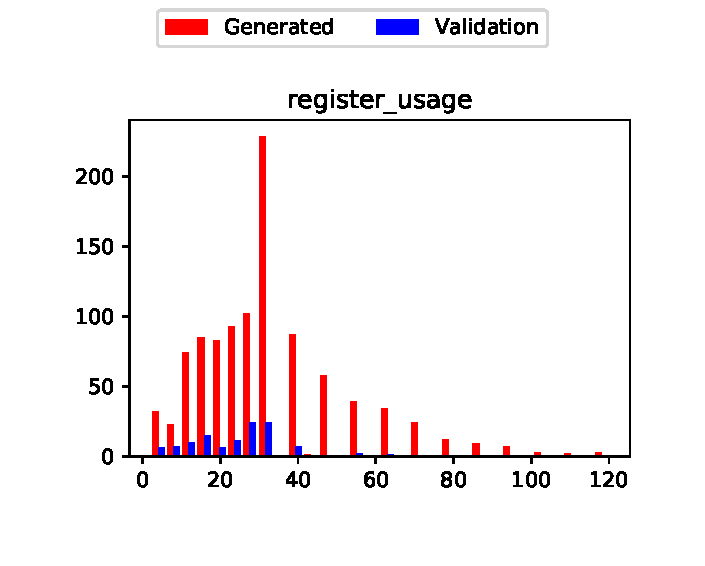
\includegraphics[width=0.85\columnwidth]{images/gen_vs_val_reg_usage.pdf}
  \caption{ A comparison between register usage in generated and validation
  stencils expressed in absolute numbers. The generated dataset contains 1200
  samples while validation one 113.}
  \label{fig:gen_cs_val_reg_usage}
\end{figure}

\paragraph{Input space coverage} As already shown in figure
\ref{fig:gen_vs_val_top_features}, we are able to replicate the properties of
validation dataset quite accurately. Here we are going to analyze the input
space for each of the most relevant features and a way of influencing it.

By experimenting with stencils of various lengths, we identified \textbf{120}
as the maximal and \textbf{2} as the minimal number of registers that
\texttt{nvcc} allocates. Furthermore, we observed, that in the interval
$\interval[{4, 32}]$ any number of registers can be allocated while in
$\interval[{33, 120}]$ range most of the numbers are never picked. Figure
\ref{fig:gen_cs_val_reg_usage} shows the comparison of register usage between
generated and validation data in absolute terms. The most common number of
allocated registers is 32 (157 times), followed by 30 (67 times).

\begin{figure}
  \centering
  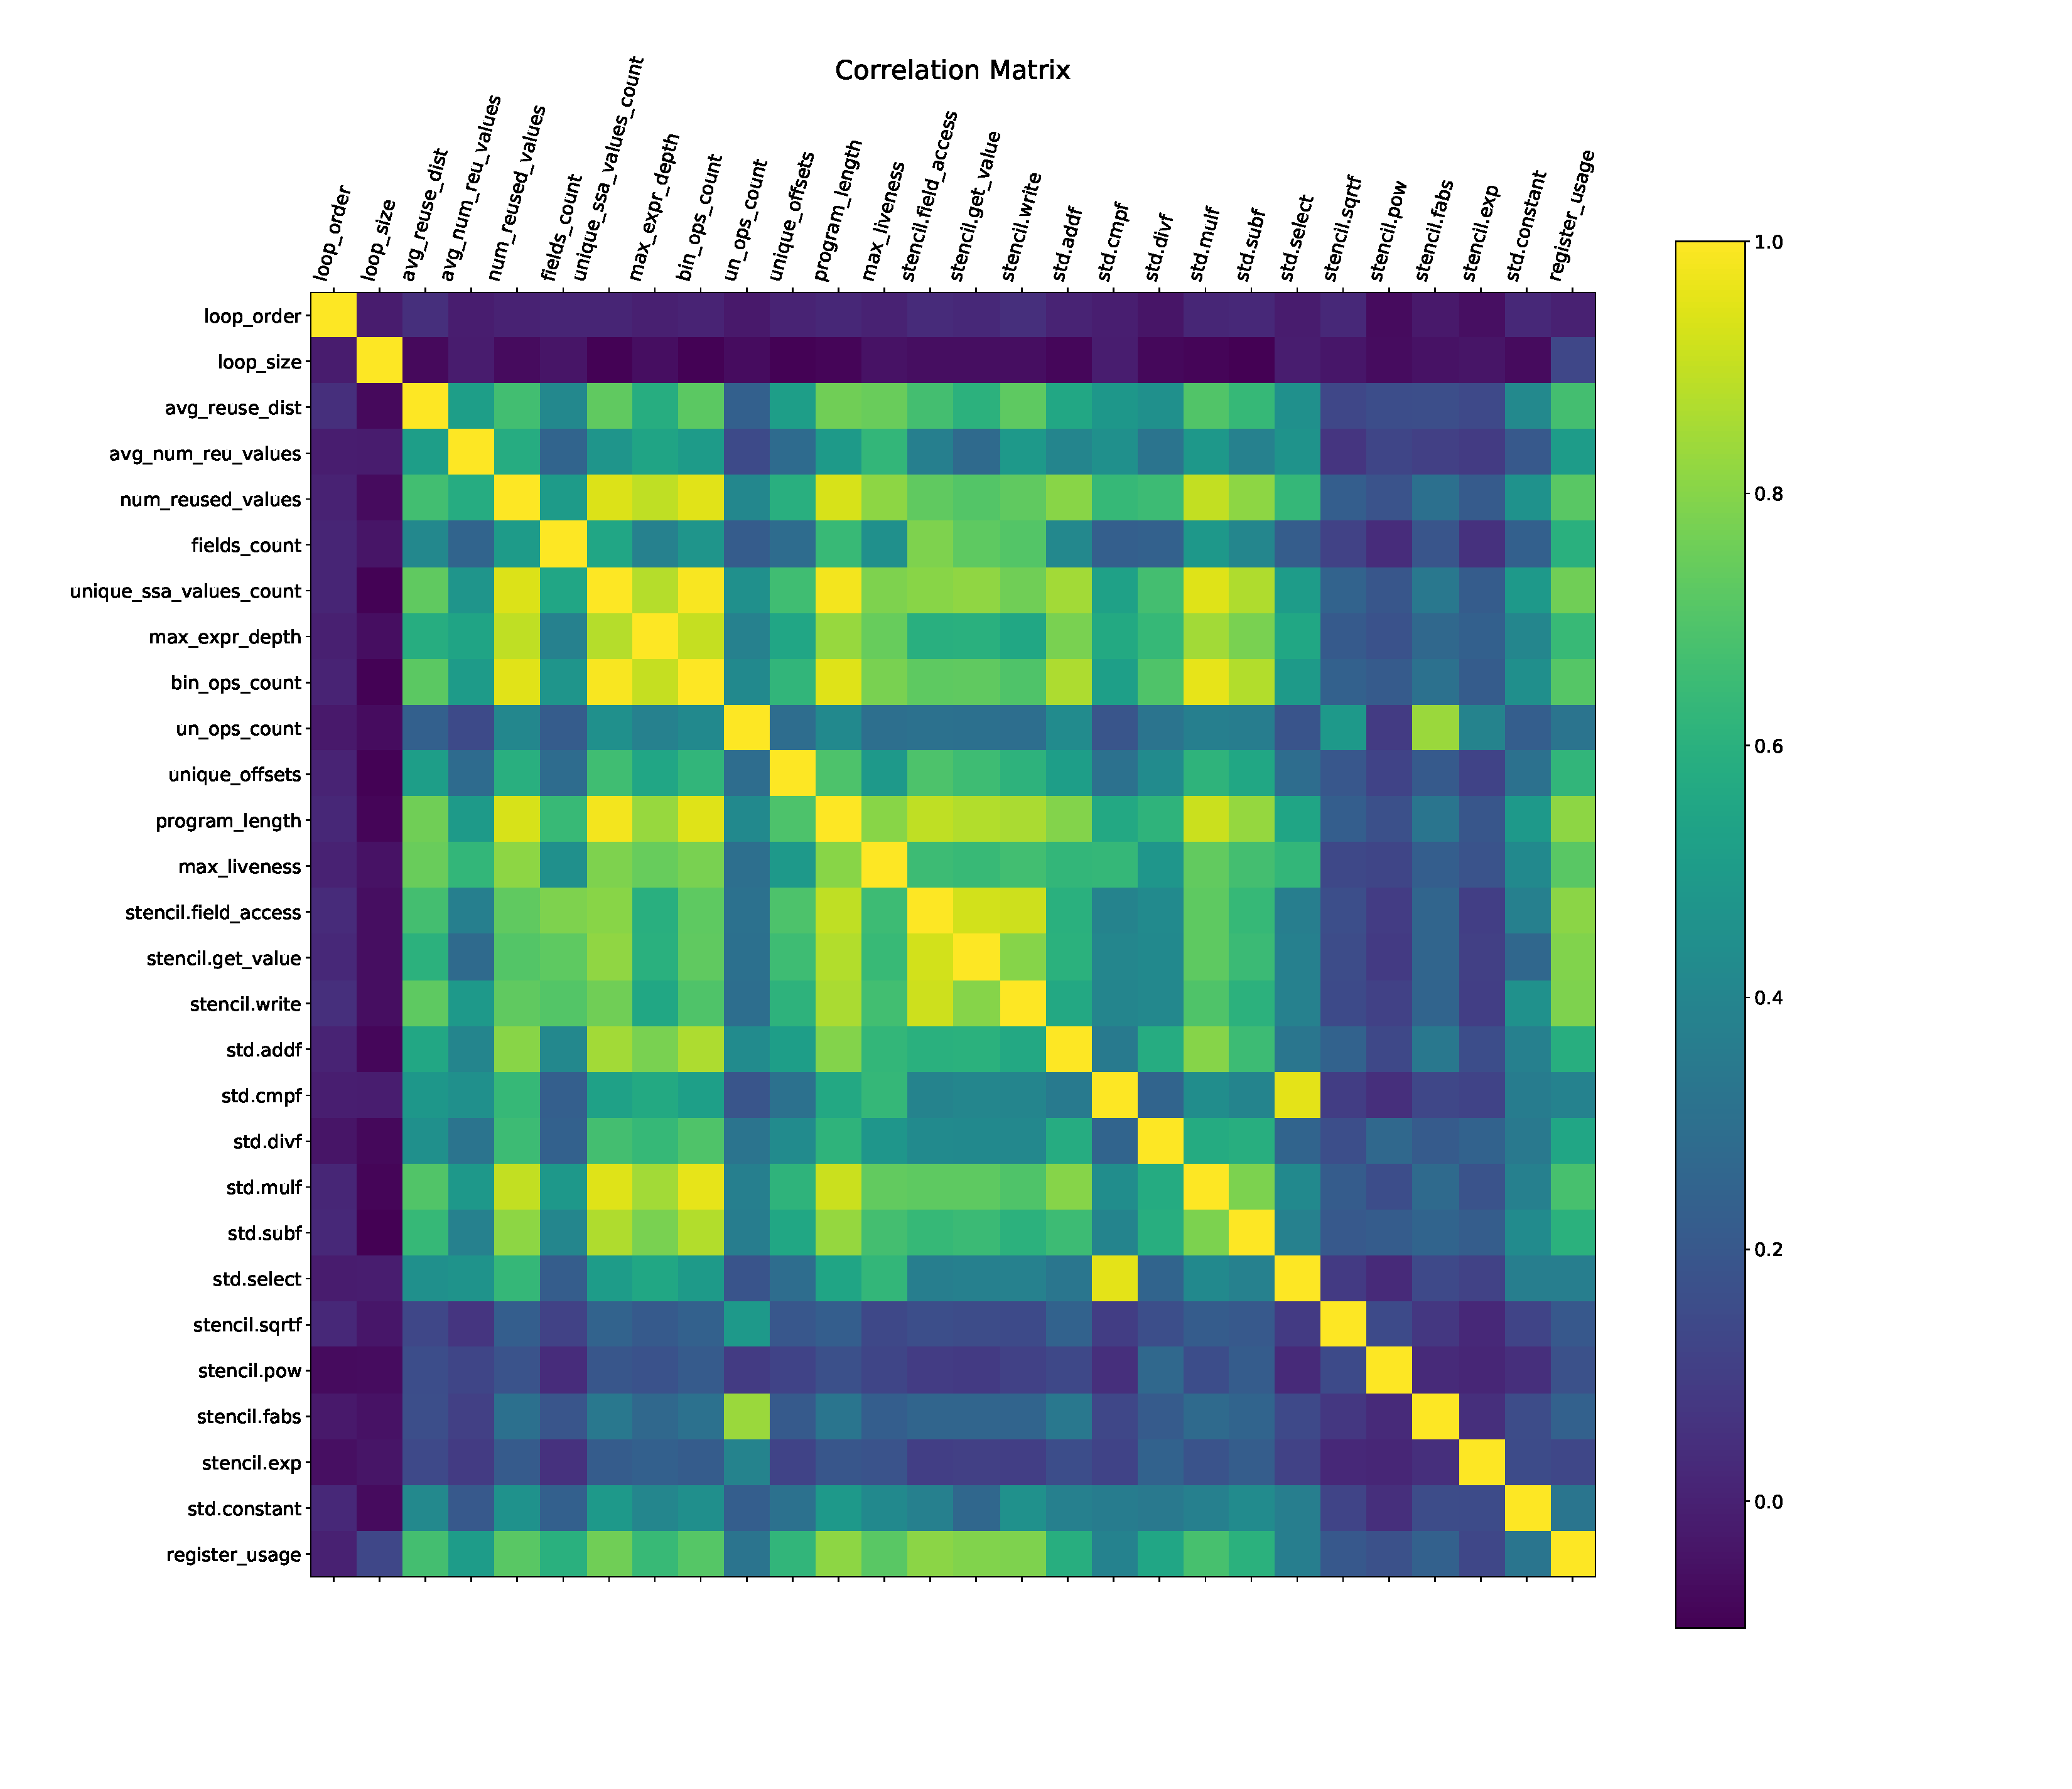
\includegraphics[width=\columnwidth]{images/corr.pdf}
  \caption{A correlation matrix of the generated dataset showing how strong
  relationships between the features are. Especially relevant is the correlation
  of the register usage with other features as we are going to train models
  predicting it.}
  \label{fig:corr}
\end{figure}

As already mentioned, we can influence other features to some degree by
changing the interval of desired program length. We can see that correlation
in figure \ref{fig:corr} shows very strong dependencies between program length
and all other features except for: (1) the loop size and order, which are
completely independent of program length as they don't represent operation
quantities, (2) unary operations which occur rarely in the programs, and (3)
the average number of reused values, which is influenced by distribution for
value selection. The relationship of program length with other features shows
that our generator can reproduce properties of any input dataset by searching
for the optimal interval of program length.

\begin{center}
  \begin{tabular}{ l c c c c c c c r }
  \hline
  \thead{Size} & \thead{MSE$_f$} & \thead{Mean$_f$} & \thead{Med$_f$} &
  \thead{STD$_f$} & \thead{MSE} & \thead{Mean} & \thead{Med} &
  \thead{STD}\\
  \hline
  100 & 22.868 & 3.254 & 2.391 & 3.504 & 40.251 & 4.099 & 1.881 & 4.842\\
  200 & 25.102 & 3.345 & 2.361 & 3.73 & 55.601 & 4.962 & 3.183 & 5.566\\
  500 & 18.093 & 2.598 & 1.572 & 3.368 & 62.255 & 4.765 & 1.728 & 6.288\\
  750 & 19.591 & 2.55 & 1.266 & 3.618 & 73.716 & 5.146 & 1.892 & 6.873\\
  1000 & 16.293 & 2.351 & 1.363 & 3.281 & 69.439 & 5.046 & 1.65 & 6.631\\
  \rowcolor{lightgray} 1200 & 16.173 & 2.384 & \textbf{1.153} & 3.238 & 58.374 & 4.671 & \textbf{1.486} & 6.045\\
  1500 & 16.518 & 2.509 & 1.29 & 3.197 & 75.666 & 5.385 & 1.743 & 6.831\\
  1750 & 16.702 & 2.422 & 1.209 & 3.291 & 64.288 & 4.975 & 1.656 & 6.288\\
  2000 & 17.2 & 2.507 & 1.229 & 3.304 & 65.617 & 5.075 & 2.226 & 6.313\\
  5000 & 17.335 & 2.584 & 1.714 & 3.265 & 58.809 & 4.929 & 2.031 & 5.874\\
  10000 & 17.001 & 2.454 & 1.469 & 3.313 & 53.169 & 4.67 & 2.262 & 5.6\\
  12000 & 17.14 & 2.617 & 1.782 & 3.208 & 58.25 & 4.74 & 2.311 & 5.981\\
  15000 & 16.062 & 2.477 & 1.663 & 3.15 & 54.76 & 4.565 & 2.167 & 5.824\\
  20000 & 15.335 & 2.418 & 1.693 & 3.08 & 47.115 & 4.227 & 2.1 & 5.408\\
  25000 & 16.914 & 2.555 & 1.736 & 3.223 & 46.543 & 4.244 & 2.066 & 5.342\\
  30000 & 16.146 & 2.433 & 1.606 & 3.197 & 49.523 & 4.393 & 2.355 & 5.497\\
  \hline
  \end{tabular}
  \captionof{table}{An accuracy of focused ($_f$) and fully trained GBT
  model for different dataset sizes. We measured the accuracy always on
  the same dataset of validation (COSMO) stencils that have 113 samples.}
  \label{tab:gbt_search_size}
\end{center}

\paragraph{Dataset size} The second property and from our perspective, the
most important one is dataset size. With dataset size, we can influence input
space coverage as a bigger dataset has a higher chance of covering the
properties of validation one. Furthermore, more data can improve model training
as they cover the input and output space better. However, they can cause
overfitting as well, which is something we want to avoid. Therefore, we
generated a huge dataset containing 30K stencil programs and searched for the
optimal size by training the best performing model - Gradient Boosting Trees
(GBT) on the subsampled data of various sizes. The results of the search are
summarized in table  \ref{tab:gbt_search_size}. We rerun the experiment five
times for each size with always newly uniformly subsampled data and took an
average. It turned out that five reruns are enough as we observed only a small
variance between runs. Furthermore, we did the focused training where we
trained the model only on data having register usage smaller or equal to 45.
The reason behind that is an observation that in this range model can fit the
data better than it would in the full range while covering 98\% of the register
usage space of validation data. We validated both models on the same validation
data. The results for the focused model are shown as well in table
\ref{tab:gbt_search_size} with subscript $f$. From now on, we will show all
results for the focused models, which are more accurate. The results for the
"full models" are in the appendix.

\begin{figure}
  \centering
  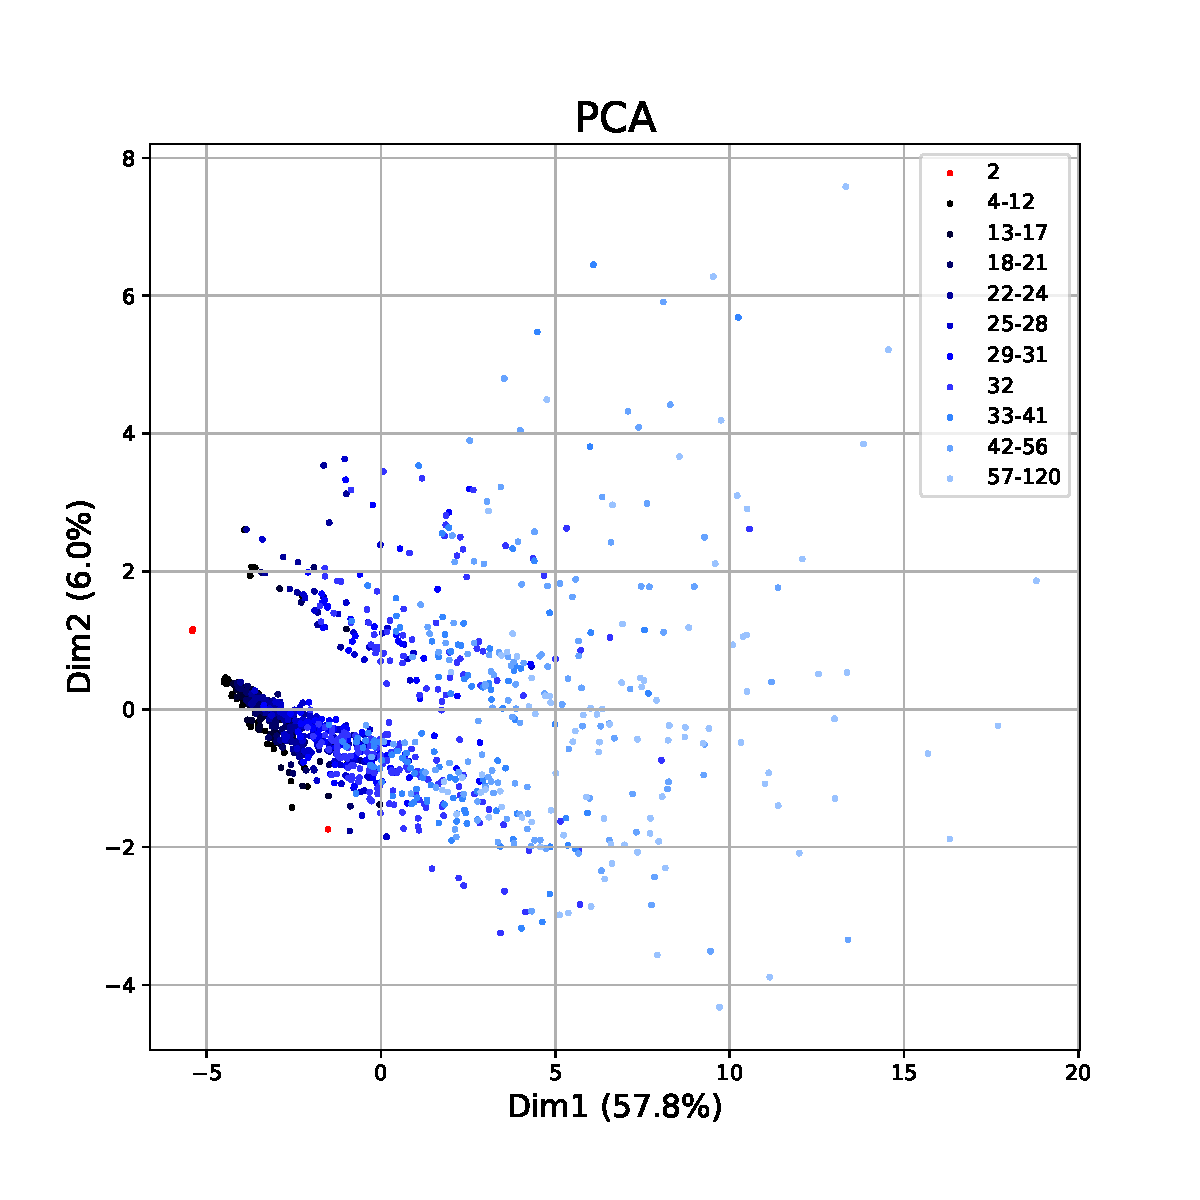
\includegraphics[width=0.9\columnwidth]{images/pca.pdf}
  \caption{Datapoints of the generated dataset projected to a 2D plane by
  using 2 most dominant principal components. The first two components
  maximize variance and thus capture almost 64\% of all variance.}
  \label{fig:pca}
\end{figure}

\paragraph{Dimensionality} Figure \ref{fig:pca} shows a projection of the
high-dimensional, optimized random stencil dataset to a 2D plane. To do the
projection, we had to reduce dataset dimensions from 26 to 2. We used PCA for
dimensionality reduction and selected 2 most dominant principal components.
The color of each data point depends on its register usage. Since the range
of possible register usages is extensive, we decided for the split into smaller
intervals with evenly distributed data points

\begin{figure}
  \centering
  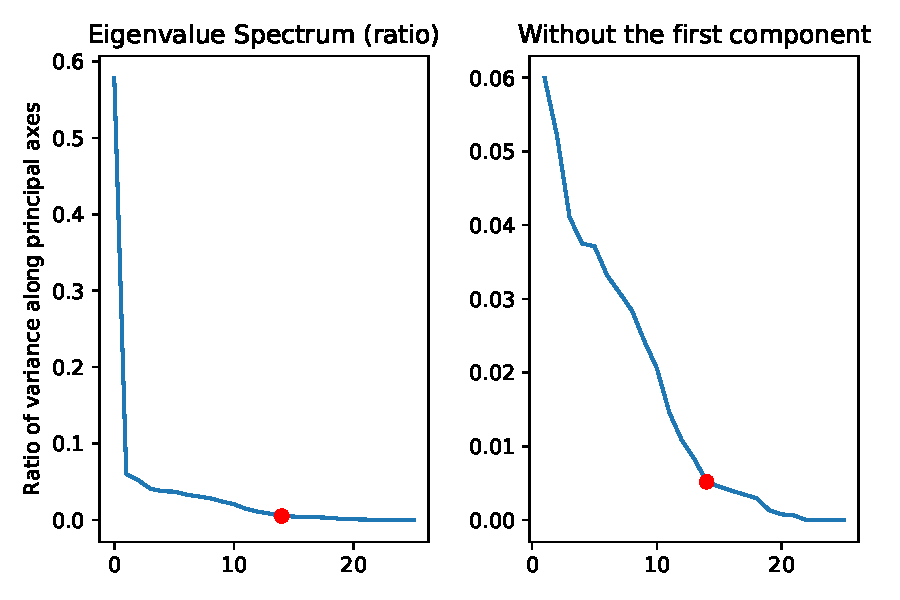
\includegraphics[width=0.9\columnwidth]{images/eigenvalues.pdf}
  \caption{ Eigenvalue Spectrum ratio shows how much variance is across
  principal components. The most dominant one takes more than a half (57.8\%)
  of it, followed by the significant drop until it stops in the 14th
  eigenvalue (red dot), which is the "knee" in the eigenspectrum, i.e.,
  the first of components that we do not keep among the set of reduced
  dimensions. The first 13 components contain $\approx 98\%$ of all variance,
  and thus the reconstruction error is $\approx 2\%$, which means that the
  dataset has low to medium dimensionality. }
  \label{fig:eigenvalues}
\end{figure}

It is interesting to observe how data points in figure \ref{fig:pca} are
getting sparser together with the increase in register usage, which implies
that they have higher dimensionality as well as the reconstruction error.
It is logical as these programs tend to be longer and have more difficult
structures, which require more features to express. Therefore high register
usage programs make training more challenging to converge as models have to
distribute weights among more dimensions. Furthermore, they enlarge output
space, which makes data fitting more complex.

The red dots in figure \ref{fig:pca} represent stencils using only 2 registers.
These stencils got eliminated either by our optimization passes or by
\texttt{nvcc}. Even though they are all empty and thus have all essential
features the same, PCA projects one data point among nonempty stencils. The
reason behind it is that our optimization passes did not eliminate this
stencil's body away, but \texttt{nvcc} managed to. Therefore the feature
vector of this stencil contains a lot of noise as dead code regions influence
most of the features, which \texttt{nvcc} eliminates. After a small
investigation of this case, we found that our constant propagation pass had
some space for improvement, but we decided to keep it as a demonstration of
PCA usefulness in dataset visualization and investigation.

Figure \ref{fig:eigenvalues} displays an eigenvalue spectrum. Since PCA tries
to maximize variance for every principal component, given that they have to
be orthogonal to each other, we can see a massive drop of variance starting
from the second component. The drop is no surprise as the first component
has to have the largest possible variance. Therefore, we can simultaneously
maximize variance and minimize the number of dimensions by identifying a
"knee" in the Eigenvalue spectrum and keeping all components in front of it.
In the case of this spectrum, the "knee" lies in the 14th component, and thus
we can express $\approx 98\%$ of all variance in only 13 dimensions, which is
half of the original dimensions.

Based on all of the points discussed above, we concluded that the dataset of
1200 optimized random stencil programs is the most suited one for the register
usage prediction. Figures evaluating some of the other datasets are in the
appendix.

\subsection{Predicting Register Usage}

Register usage provides a piece of essential information for compiler
optimization. If we could obtain a register usage of any stencil program in
order of milliseconds, we would be able to try multiple optimization
strategies and pick the one using the smallest amount of registers and thus
eliminate high register pressure. However, the time it takes \texttt{nvcc}
to produce register usage information does not allow a broad search for the
best optimization. Therefore, we decided to circumvent \texttt{nvcc} by
training machine learning models that can predict register usage much faster.

Since our datasets have low dimensionality and small input space, we decided
to use simple statistical models, which are easy and fast to train and work
well with small training datasets. In particular, we decided to use
\textit{Ridge Regression} as a baseline model and
\textit{Gradient Boosting Trees} as the second model. In the following
subchapters, we are going to explain how both models work and the results
we achieved using them.

We identified register usage prediction as a regression \cite{regression}
problem. In regression analysis, we try to estimate the relationship between
dependant variables (in our case only one - register usage) or \textbf{y}, and
independent variables called input variables or \textbf{X}, which are in our
case collected features. In other words, we want to automatically find how
stencil features influence the number of allocated registers. Furthermore,
we want to leverage this knowledge in predicting new, unseen data. 

In the linear regression, we are searching for the line that best fits the
data according to the given error function. In other words, we want the line
that minimizes the distance between the predicted values and the actual values.
More formally this optimization problem can be defined as:
\begin{equation}
\min \frac{1}{n} \sum_i (\hat{y}_i - y_i)^2
\end{equation}
\noindent where

\begin{itemize}
  \item []$\hat{y}_i$ is the predicted value
  \item []$y_i$ is the actual value
  \item []$n$ is the number of samples
\end{itemize}
\noindent and we try to minimize the \textit{mean squared error} (MSE) -
that is, the average squared difference between predicted and actual values.

\begin{figure}
  \centering
  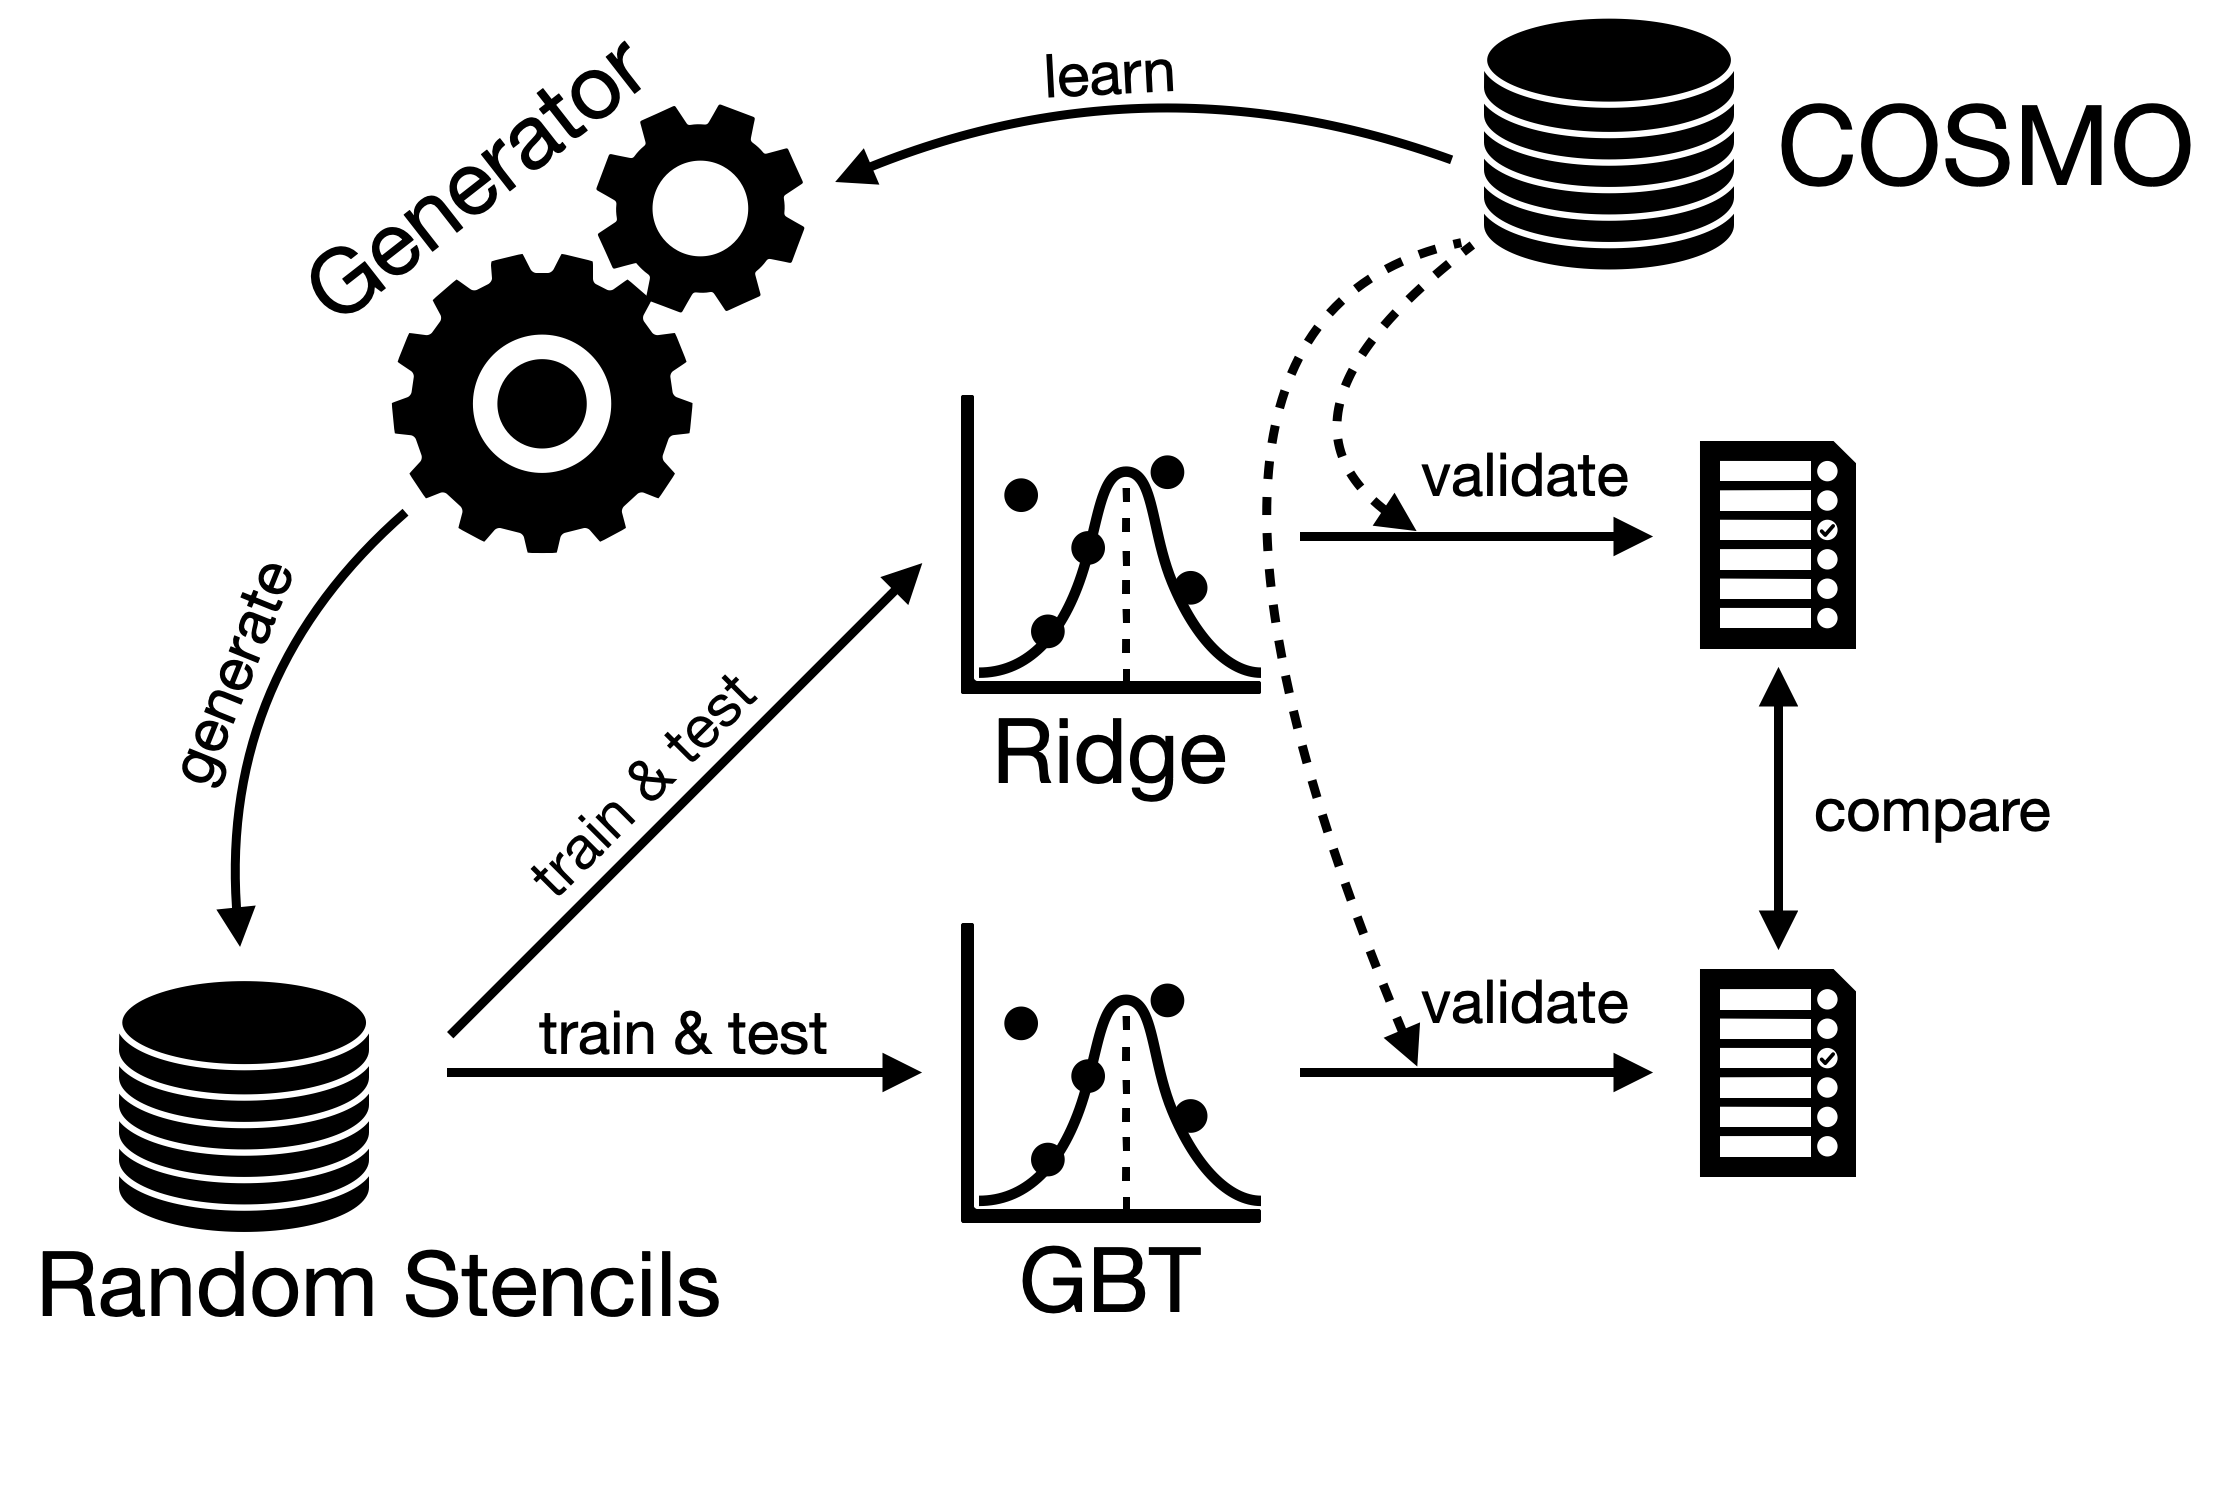
\includegraphics[width=0.9\columnwidth]{images/reg_pred_diagram.png}
  \caption{Diagram shows a high-level overview of the register prediction
  pipeline. The important note is that we never train on COSMO data directly.
  They are always used only for validation.}
  \label{fig:reg_pred_diagram}
\end{figure}

% motivation
% comparing regression with GBT
% accuracy evaluation
% timing evaluation

\subsubsection{Ridge Regression}

Tikhonov regularization or ridge regression is a well-known regularization
method of ill-posed problems. It solves a regression problem where the loss
function is linear least squares, and it uses l2-norm as a regularization.
Therefore the objective function is:
\begin{equation}
||y - Xw||^2_2 + \alpha ||w||^2_2
\end{equation}

\noindent which has only one hyperparameter $\alpha$ - a regularization
strength (must be a positive number). $X$ denotes the input data (independent
variables) and $y$ the independent variables. The model tries to find the
optimal vector of weights $w$, whose product with $X$ minimizes the least
squares \cite{least_squares} loss function. $\alpha$ reduces the variance
of the predicting values as well as improves conditioning.

We run the model with different $\alpha$ values and results are summarized
in table \ref{tab:ridge}.

In our experiment, we used the scikit learn implementation of the algorithm,
which one can find here \cite{scikit_ridge}. For more information about the
regression itself, we recommend to follow up here \cite{wiki_ridge}.

\begin{center}
  \begin{tabular}{ l c r }
  \hline
  \thead{Mean} & \thead{Std} & \thead{$\alpha$} \\
  \hline
  -14.305176 & 2.757947 & 0.25 \\
  -14.298890 & 2.749494 & 0.5 \\
  -14.287009 & 2.733225 & 1.0 \\
  -14.265767 & 2.702987 & 2.0 \\
  -14.231775 & 2.650073 & 4.0 \\
  -14.188361 & 2.565548 & 8.0 \\
  -14.156424 & 2.444302 & 16.0 \\
  \hline
  \label{tab:ridge}
  \end{tabular}
  \captionof{table}{Grid search for the optimal $\alpha$ value. Table shows
  MSE, the mean and standard deviation for different $\alpha$ values with
  10-fold cross-validation of the Ridge regression model.}
\end{center}

\begin{figure}
  \centering
  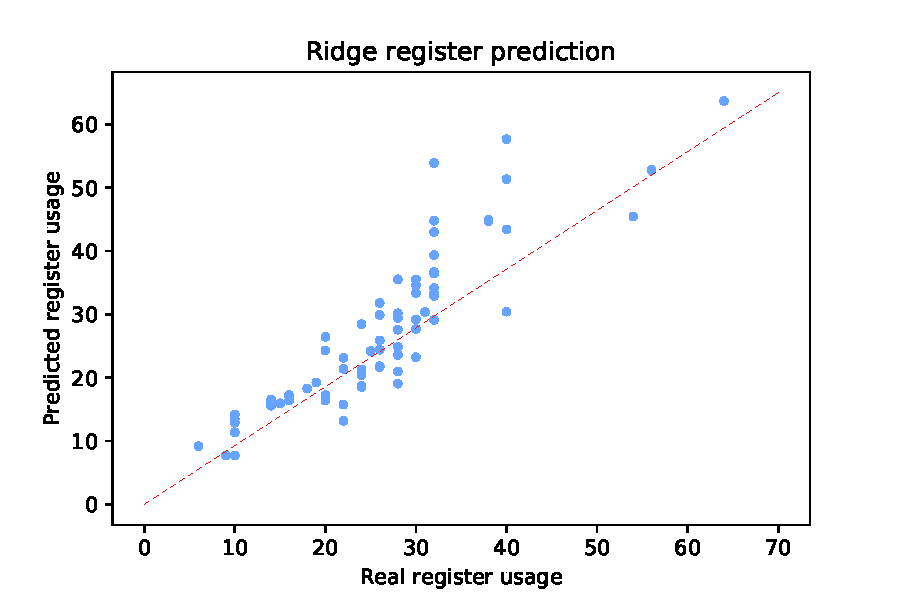
\includegraphics[width=\columnwidth]{images/ridge_pred.pdf}
  \caption{Scatter plot target vs predicted values. Prediction results are
  very accurate for programs with low register usage. However, the accuracy
  is dropping as the number of registers increases.}
  \label{fig:ridge_pred}
\end{figure}

%Ridge Median: 2.7656012952999594 STD: 3.4754747568158355 Average: 3.538682076354835
Figure \ref{fig:ridge_pred} shows the prediction accuracy. The closer a point
is to the red dashed line, the more accurately it was predicted. We can see
that accuracy is dropping as the number of registers increases. We think that
it is caused by the higher dimensionality of the programs with high register
usage, as shown in figure \ref{fig:pca}. However, few exceptions were
predicted accurately despite their high register usage. The median prediction
error is 2.7656, the average 3.539, and the standard deviation 3.475. These
numbers are our baseline, even if we already consider them accurate enough.

\begin{figure}
  \centering
  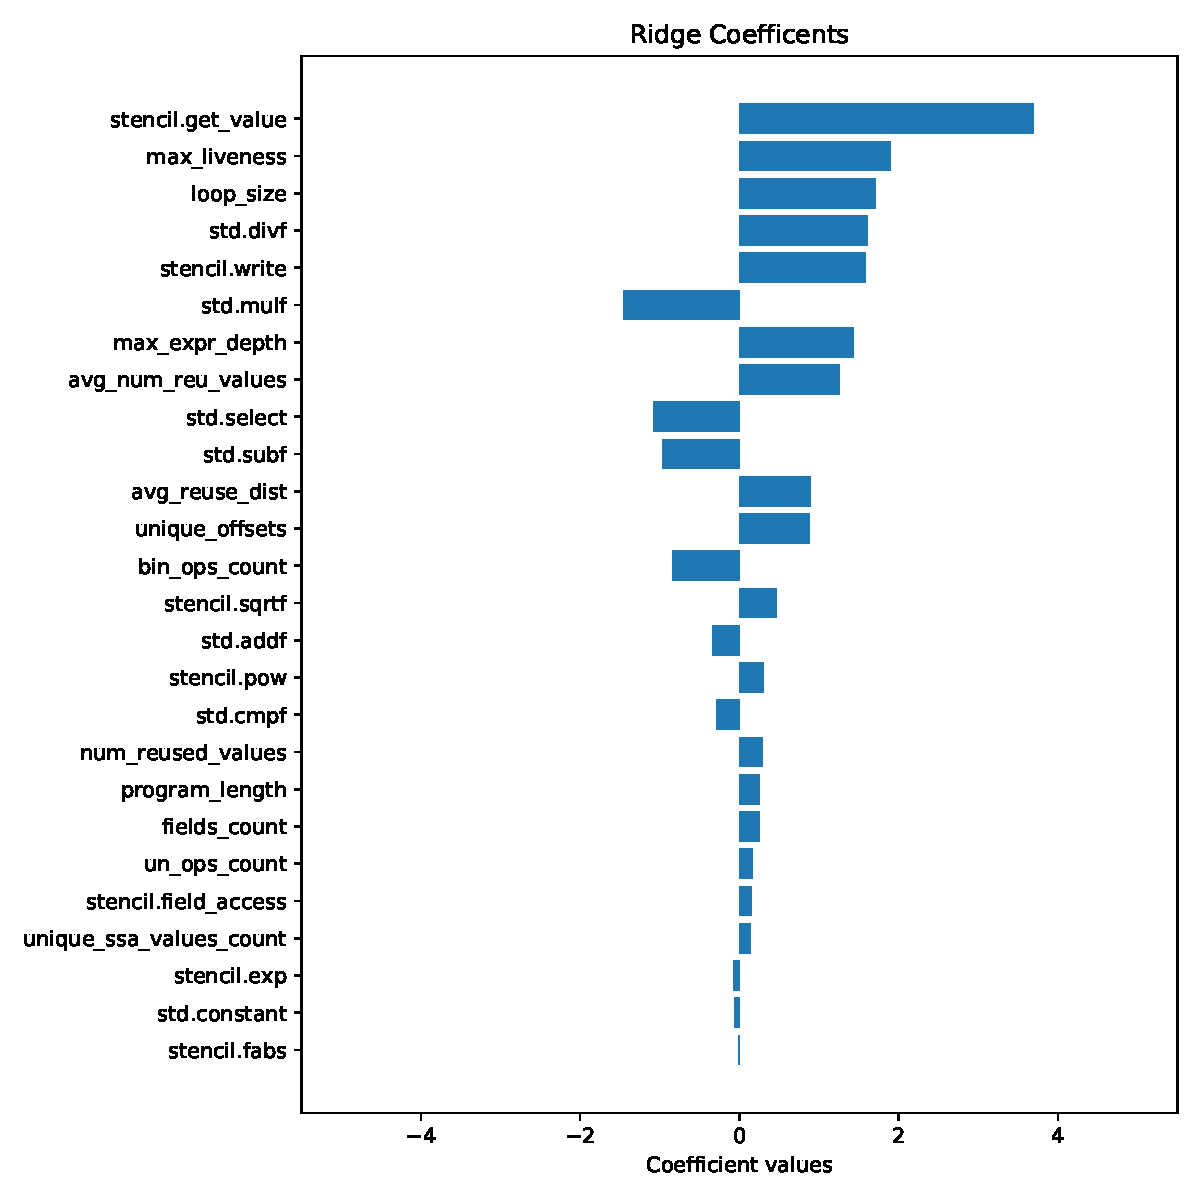
\includegraphics[width=\columnwidth]{images/ridge_var_importance.pdf}
  \caption{The ridge weight vector with coefficients. Their absolute
  values indicate variable importance to Ridge regression because
  higher value influences the resulting number more.}
  \label{fig:ridge_var_importance}
\end{figure}

Figure \ref{fig:ridge_var_importance} shows weights that Ridge regression
assigns to the features. The model makes pointer dereferencing - 
\texttt{stencil.get\_value} the most valuable feature, followed by a
\texttt{max\_liveness} and a \texttt{loop\_size}. It is quite logical as
pointer dereferencing produces a value that resides in a register, and
\texttt{max\_liveness} determines the maximum amount of values that need to
be live at the same time and thus should ideally be put in registers as well.
However, \texttt{loop\_size} makes a little sense since we prohibited loop
unrolling optimization inside the \texttt{nvcc}, and thus only the body of the
for loop matters in terms of register usage. The following features - a
division and a write, are logical as well. A division requires more registers
than any other binary operation, and a write computes the index, loads the
value, and stores it, which is demanding on the number of registers as well.
The unique offsets feature indicates the actual number of offsets that compiler
computes as it eliminates the computation of redundant offsets. Furthermore,
features related to reuse distance express how many values operations reuse
and thus should be kept in registers. The \texttt{avg\_reuse\_dist} indicates
that values with long reuse distances kept in registers are good candidates
for register spilling. The \texttt{avg\_num\_reu\_values} and
\texttt{num\_reused\_values} represent values that should ideally reside in
registers to prevent duplicate loading. Most of the other features have lower
importance either because they have lower occurrence rates in learning
programs or because the model was not able to find a strong connection between
them and register usage.

\begin{figure}
  \centering
  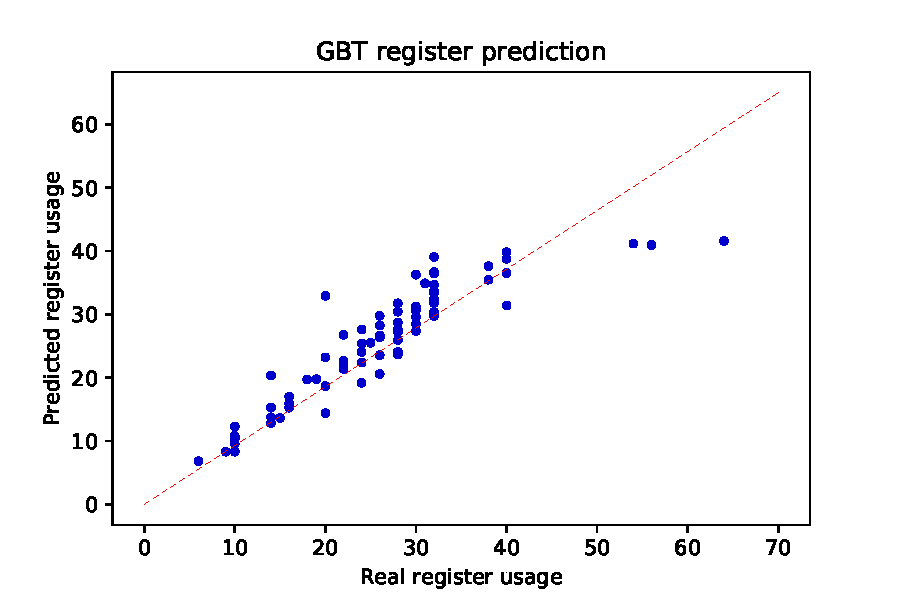
\includegraphics[width=\columnwidth]{images/gbt_pred.pdf}
  \caption{Scatter plot target vs predicted values. GBT model produces
  more accurate prediction results than Ridge regression. Furthermore,
  GBT is not only accurate for programs with low register usage, but it
  produces reliable results for stencils with medium register usage as well.
  However, prediction for the three stencils with the highest register usage
  is still inaccurate due to focused learning.}
  \label{fig:gbt_pred}
\end{figure}

\subsubsection{Gradient Boosting Trees}

The second model we tried is Gradient Boosting Trees (GBT). We picked this
algorithm as it often produces the best predictive performance by connecting
fixed size decision trees with gradient boosting. This way, it combines many
usually weak learners into a single strong one. The gradient boosting is
iterative functional gradient descent, which optimizes a given loss function
by iteratively choosing the negative direction of the gradient.  It is very
easy to train as default hyperparameter values usually work well. In our
approach, we used the implementation from scikit learn \cite{scikit_gbt} and
more information about the algorithm can be found here \cite{friedman2001},
\cite{wiki_gbt}.

\begin{figure}
  \centering
  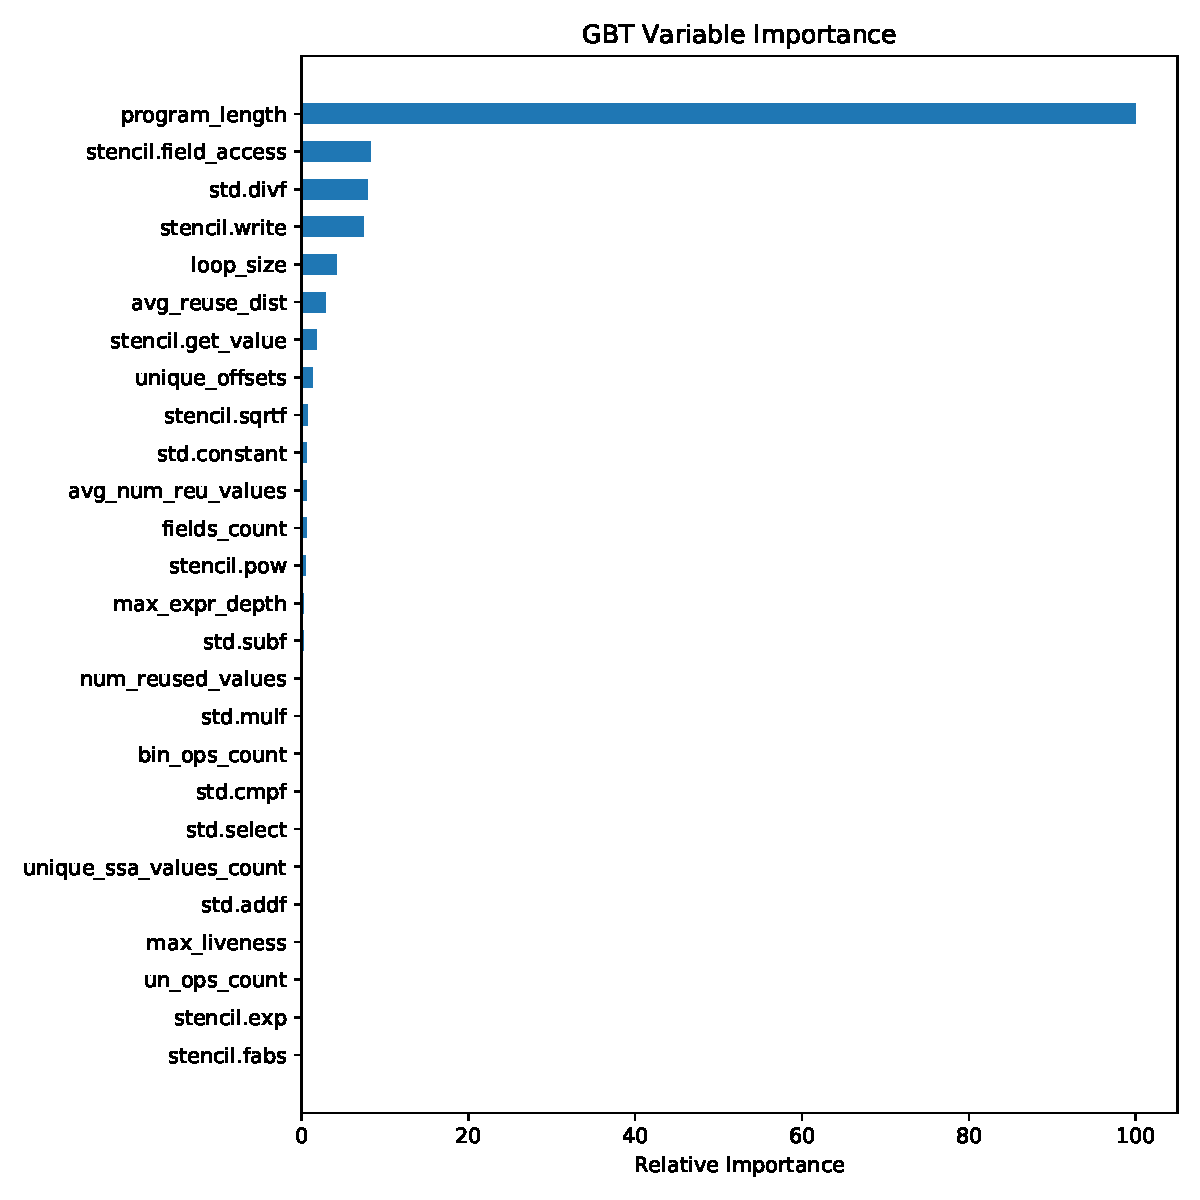
\includegraphics[width=\columnwidth]{images/gbt_var_importance.pdf}
  \caption{Figure shows how the \texttt{program\_length} dominates in GBT
  weights by wide margin.}
  \label{fig:gbt_var_importance}
\end{figure}

%GBT Median: 1.1533388196451408 STD: 3.2591677227867963 Average: 2.381004639468263
The average accuracy on the validation data is 2.384, median 1.153, and a
standard deviation of 3.238. All of these values are better than the ones of
Ridge regression. Furthermore, median accuracy improved 2.4 times. We
expected this improvement as GBT has one of the best prediction accuracies in
this field of machine learning. Figure \ref{fig:gbt_pred} shows a scatter plot
with prediction accuracy for the individual validation stencils. The model is,
unlike Ridge regression, accurate for both low and high register usage
stencils. The only exceptions are three stencils with the highest register
usage that GBT predicted inaccurately as its training focused on low and
medium register usage stencils. However, unfocused training can predict those
accurately as well but overall is slightly less accurate, as can be seen in
table \ref{tab:gbt_search_size}.

Figure \ref{fig:gbt_var_importance} shows variable importance inside GBT. We
can see that the model has chosen a completely different approach as the Ridge
regression since it put most of the weight on \texttt{program\_length} while
Ridge regression treated it as an unimportant feature. The reason behind that
might be that we focused the training on stencils with lower and medium
register usage where dependency between program length and register usage is
stronger than in high register usage stencils. Furthermore, register usage has
the highest correlation with program length, which influences GBT as well.
Division and write operations were selected as important features in this
model as well, which is logical. Unfortunately, the GBT model does not tell
us anything about the relationship between these features nor signs of their
impact or magnitude. Therefore it is hard to infer more information about
model decisions.

\subsection{Speed Comparison}

Figure \ref{fig:nvcc_vs_gbt} shows a speed comparison between GBT
and \texttt{nvcc}. As expected, GBT is a clear winner. It is more than 50
times faster than \texttt{nvcc} because it just multiplies learned weights
with a feature vector, whereas \texttt{nvcc} has to perform all kinds of
analyses. Therefore we conclude that register prediction should have its
place in stencil optimization as it outperforms traditional analyses,
and its accuracy is acceptable.

\begin{figure}
  \centering
  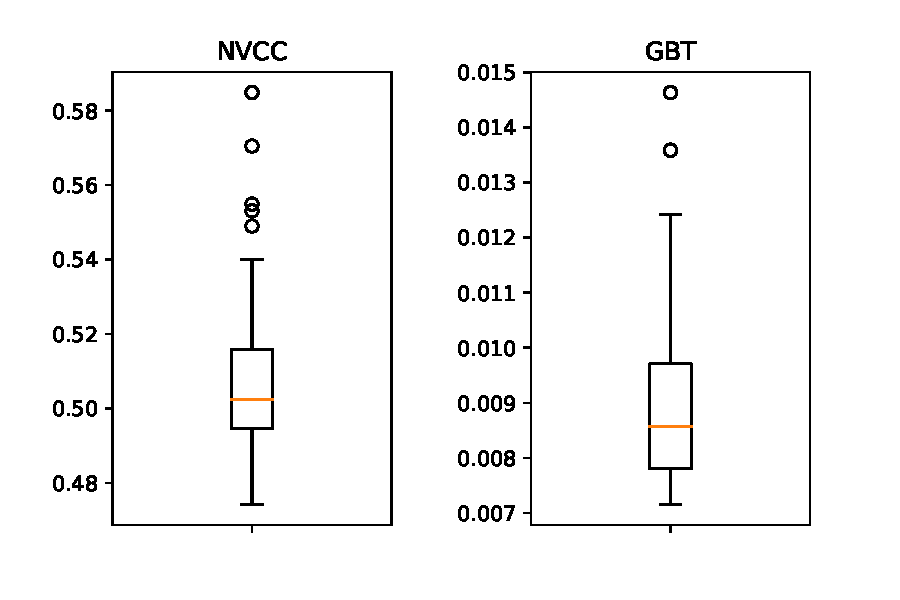
\includegraphics[width=0.8\columnwidth]{images/nvcc_vs_gbt.pdf}
  \caption{Runtime comparison of \texttt{nvcc} with the GBT model
  that is, on average more than 50 times fasters. We measured
  runtimes of both methods 20 times for each validation stencil
  and took the average. The figure shows confidence
  intervals of the resulting measurements. }
  \label{fig:nvcc_vs_gbt}
\end{figure}

In this chapter, we presented the experiments we performed with generated
stencils. The first stage was data collection, which consists of a feature
vector definition and feature extraction. In the second stage, we analyzed
the collected data to understand them. Lastly, we trained two models on the
generated data and validated them on the COSMO stencils. The results show
that register prediction is more than 50 times faster than register allocation
done by \texttt{nvcc} and reliable enough to be used in future research.

\section{Related Work}
Stencils computations have been studied extensively in the last decade.
They are used heavily in many fields, including weather
simulations \cite{stella}, machine learning \cite{gpu_ml}, physical simulation
and modeling \cite{stencil_phys_sim}, deep learning \cite{tvm}, computer
vision, and image processing \cite{halide}.
Following current trends, stencil computations try to exploit parallelism
by proposing autotuning solutions for parallel stencil computations
\cite{10.1145/1989493.1989508}, \cite{5470421}, \cite{6012879},
\cite{gridtools}, that come either in the form of frameworks \cite{gridtools}
that extend existing programming languages or compilers that introduce
their own DSLs. \cite{10.1145/1989493.1989508}

Since our work focuses more on learning which optimizations to perform rather
than optimization improvement or parallelism, the more related papers are from
Ashouri et al. \cite{Ashouri_survey} and Wang et al. \cite{wang2018survey},
which both took an extensive survey on machine learning applications in
compilers. They split recent advances into two major categories: (1) Choosing
the best optimization, and (2) An order of optimization passes. Ashouri et al.
introduced COBAYN \cite{Ashouri_cobayn}, which uses Bayesian networks to
predict the optimal order of optimization passes and thus falls into the
second category. While from the long term perspective, our thesis builds a
foundation for the search of the best optimization (1st category), the short
term goal was to predict program properties like runtime or register usage,
which does not fall into these categories. Therefore, our approach is closer
to the one of Raychev et al. \cite{raychev} that predicts syntactic and
semantic properties inside the program. In particular, it focuses on
deobfuscation by learning the associations between variable names and their
locations inside the program structure.

Probably the closest approaches to ours are Autotvm from Chen et al.
\cite{autotvm} and Halide Autoscheduler from Adams et al. \cite{halide_ml}.
Both of them aim to find the optimal loop fusion and tiling by searching
the optimization space. They perform the search by employing different search
strategies (Halide - tree search, Autotvm - simulated annealing),
but both are using a ranking function, which is a pre-trained machine
learning model predicting relative runtime for each schedule based on its
features. An alternative approach is Absinthe \cite{Absinthe} from Gysi et al.,
which solves the problem of optimal parameters for loop fusion and tiling as
a linear optimization problem.

\section{Future Work}
As the future research direction, we propose to experiment more with high
register usage stencils, which require more advanced machine learning
techniques because of their higher dimensionality. Another research direction
could be to use our existing infrastructure to collect runtime of our random
stencils and train a machine learning model that predicts it. Having predictors
for both register usage and runtime would enable their usage in search of the
best optimization strategy. For example, one can decide whether to inline 2
stencils by predicting both register usage and runtime before and after
inlining. If both numbers are better for inlined stencils, then the compiler
keeps the stencil inlined. Otherwise, it undoes the inlining. Similarly, we
can use it for stage fusion and other optimizations requiring a search for
the optimal strategy. 

\section{Conclusion}

Global warming starts to threaten the entire world population. The
need for fast and accurate weather prediction systems is growing
together with a need for saving human lives by providing in time weather
warnings. Recent approaches in improving prediction systems usability
and efficiency led to the invention of stencil domain-specific languages
that abstracted away unnecessary implementation details, gave software
developers more space for optimization, and enabled domain scientists
to focus solely on their research domain. A very recent Google introduction
of MLIR enabled compiler developers to rapidly develop new DSLs by providing
extensible Intermediate Representation together with accompanying
infrastructure. This technology attracted scientists from the SPCL lab at
ETH Zurich to create a new MLIR Stencil dialect, which would create a new
platform bringing all Stencil computations and languages under one roof. 

This thesis brings many contributions to the dialect infrastructure. Firstly,
we implemented a translation of GPU and Standard Dialect into a CUDA C code,
which enabled us to run Stencil programs on the GPU. However, the main
contribution is the random stencil generator that replicates existing stencil
programs by learning their structure. Furthermore, we extended IR
infrastructure for feature extraction and collection passes that one can
utilize in the creation of new datasets. In addition to that, we implemented
two optimization passes that are cleaning programs off the noise, i.e., dead
and easily optimizable code. Lastly, we showed that datasets created by the
generator and cleaned with optimization passes are suitable for further
compiler optimization research by training simple statistical models that
can predict stencil register usage accurately. Their prediction speed is
more than 50 times faster than retrieving register usage information via
\texttt{nvcc}, which enables a search for optimal optimization parameters
in a much bigger space or various optimization decisions used in stencil
fusion or inlining.

%% Acknowledgments
\begin{acks}                            %% acks environment is optional
                                        %% contents suppressed with 'anonymous'
  %% Commands \grantsponsor{<sponsorID>}{<name>}{<url>} and
  %% \grantnum[<url>]{<sponsorID>}{<number>} should be used to
  %% acknowledge financial support and will be used by metadata
  %% extraction tools.
  This material is based upon work supported by the
  \grantsponsor{GS100000001}{National Science
    Foundation}{http://dx.doi.org/10.13039/100000001} under Grant
  No.~\grantnum{GS100000001}{nnnnnnn} and Grant
  No.~\grantnum{GS100000001}{mmmmmmm}.  Any opinions, findings, and
  conclusions or recommendations expressed in this material are those
  of the author and do not necessarily reflect the views of the
  National Science Foundation.
\end{acks}

%% Bibliography
%\bibliography{bibfile}


%% Appendix
\appendix
\section{Appendix}

Text of appendix \ldots

\end{document}
